\chapter{Health as Human Capital}

\fancyhead[L]{ECON0024}
\fancyhead[C]{Ch.3 Health as Human Capital}
\fancyhead[R]{Kuangjie Ni}
\fancyfoot[L]{\hyperlink{tableofcontents}{Back to Table of Contents}}
\fancyfoot[R]{Kuangjie Ni}

\section{Why are some of us less healthy than others?}
\begin{itemize}
        \item Bad genes
        \item Bad lifestyles
        \item Poor healthcare 
        \item Poor early environment 
        (e.g. poor parenting, mum drinking during pregnancy)
   \end{itemize}     
\section{Health spending}

        \subsection{Health spending per capita}

            \begin{figure}[H]%option [H] means "strictly here"
                \centering
                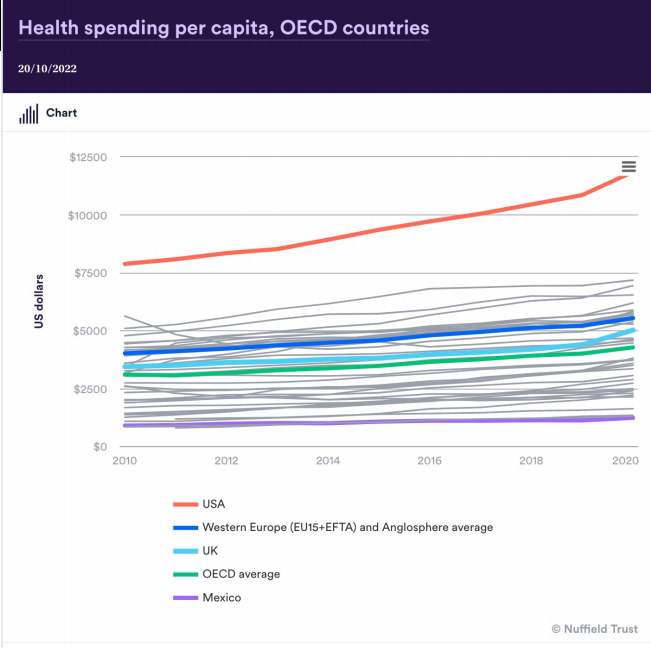
\includegraphics[width=3in]{images/ch3/1 Health spending OECD.png}
                \caption{Health spending per capita, OECD countries}
                \label{fig:label}
            \end{figure}
\begin{itemize}
        \item Health spending per capita is increasing over time. People are living longer than they used to be. The longer you live, the sicker you get and the more money you spend on healthcare. 
        \item US has a higher health spending and a particular healthcare structure.
        \end{itemize}
        
        \subsection{Health spending: Total including government/compulsory 
spending}

            \begin{figure}[H]%option [H] means "strictly here"
                \centering
                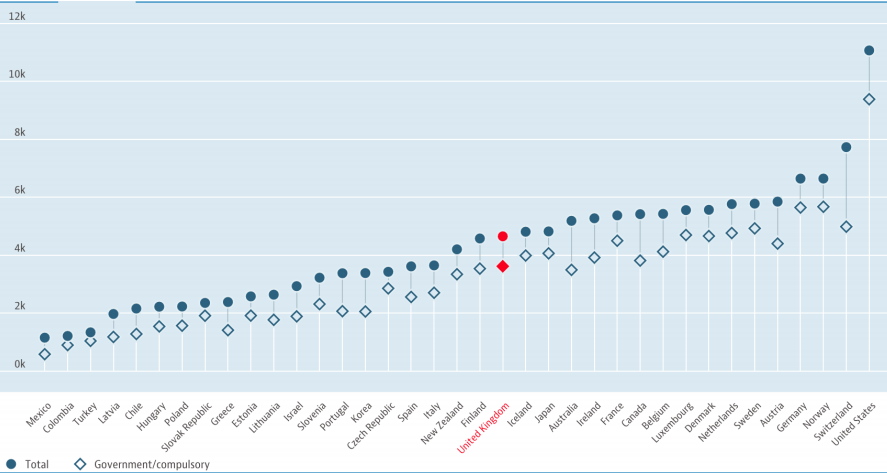
\includegraphics[width=4in]{images/ch3/2 Government.png}
                \caption{Health spending: Total including government/compulsory 
spending in US dollars/capita, 2019}
                \label{fig:label}
            \end{figure}      
\begin{itemize}
        \item Blue dots are the total health spending, and diamonds are the government/compulsory spending. 
        \item US government spends a lot of money on healthcare.
        \end{itemize}
        
        \subsection{Total spending as a proportion of GDP}
            \begin{figure}[H]%option [H] means "strictly here"
                \centering
                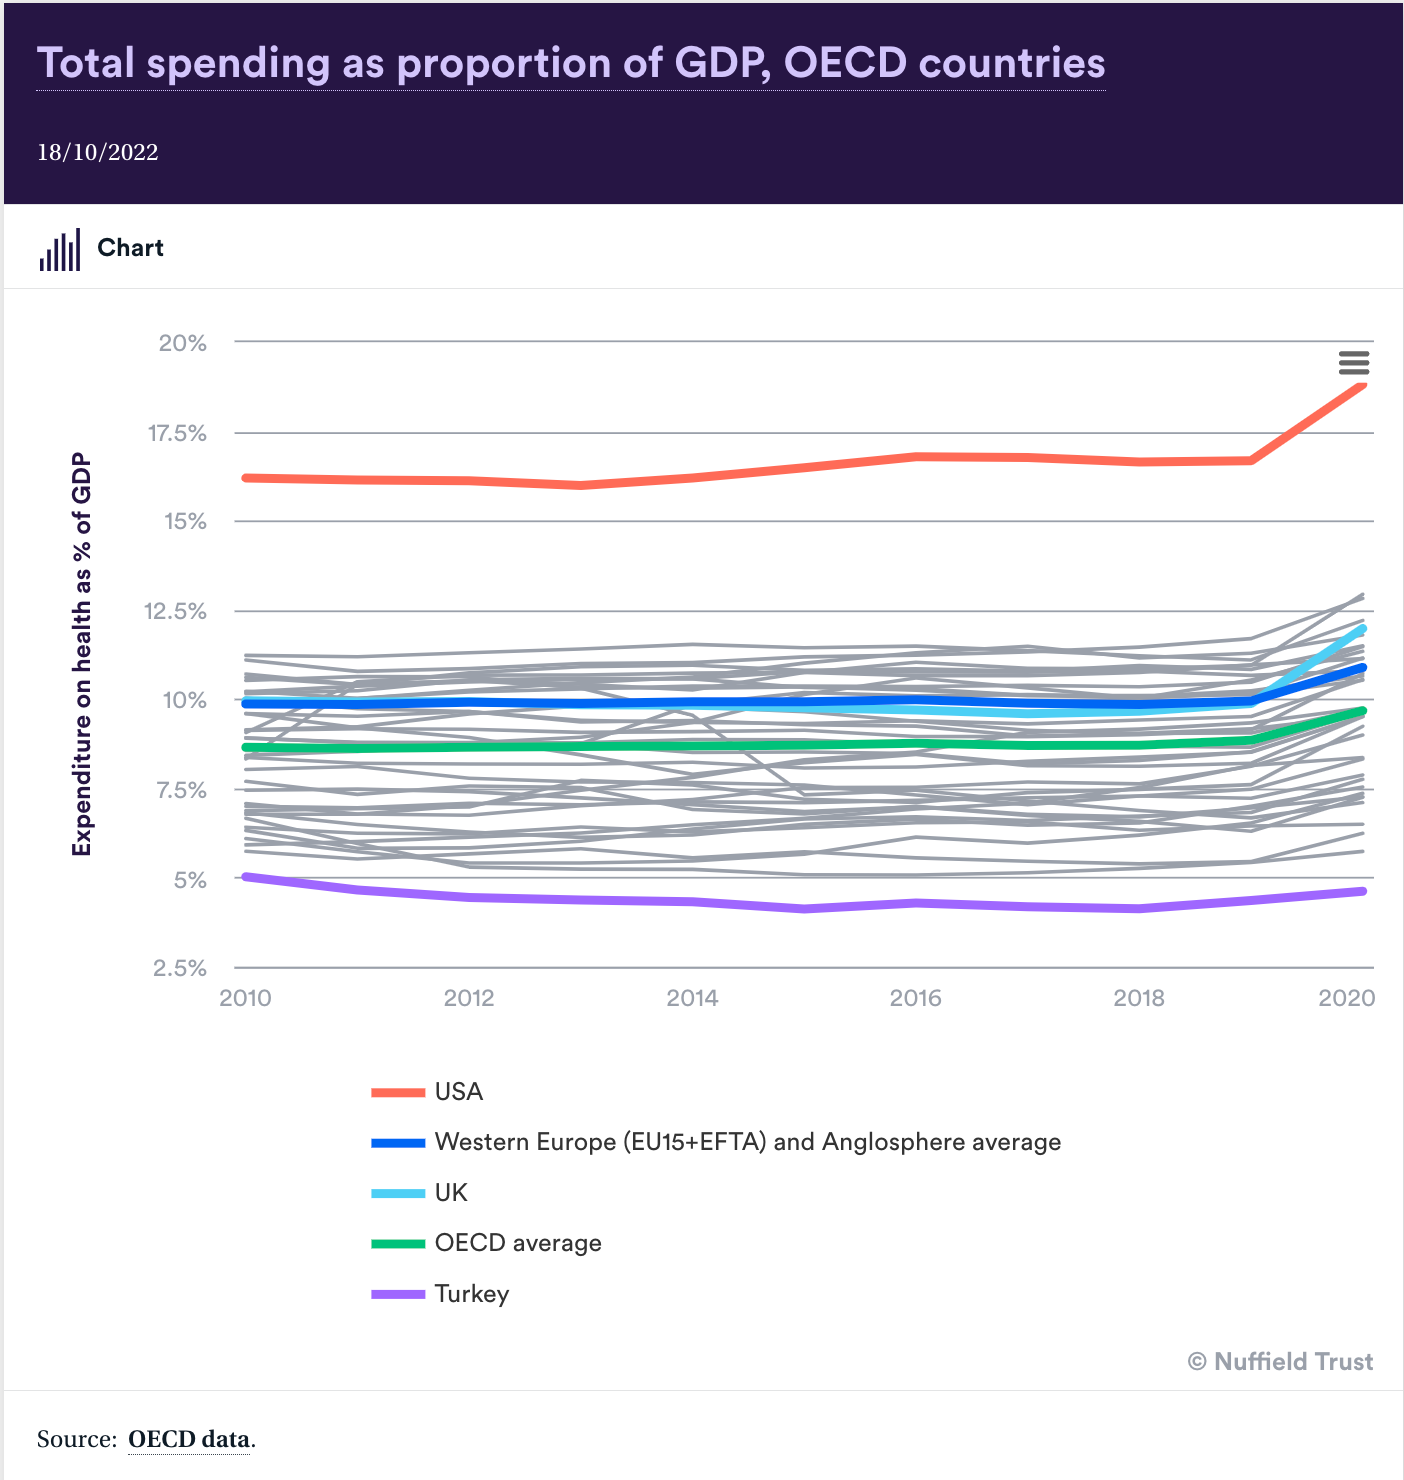
\includegraphics[width=4in]{images/ch3/3 GDP.png}
                \caption{Total spending as a proportion of GDP, OECD countries}
                \label{fig:label}
            \end{figure}            
\begin{itemize}
        \item US has the highest health spending as a proportion of GDP.
        \item The total health spending as a proportion of GDP increased during the pandemic.
        \end{itemize}
        
        \subsection{Zoom into UK: Health as a share of total UK spending}  
            \begin{figure}[H]%option [H] means "strictly here"
                \centering
                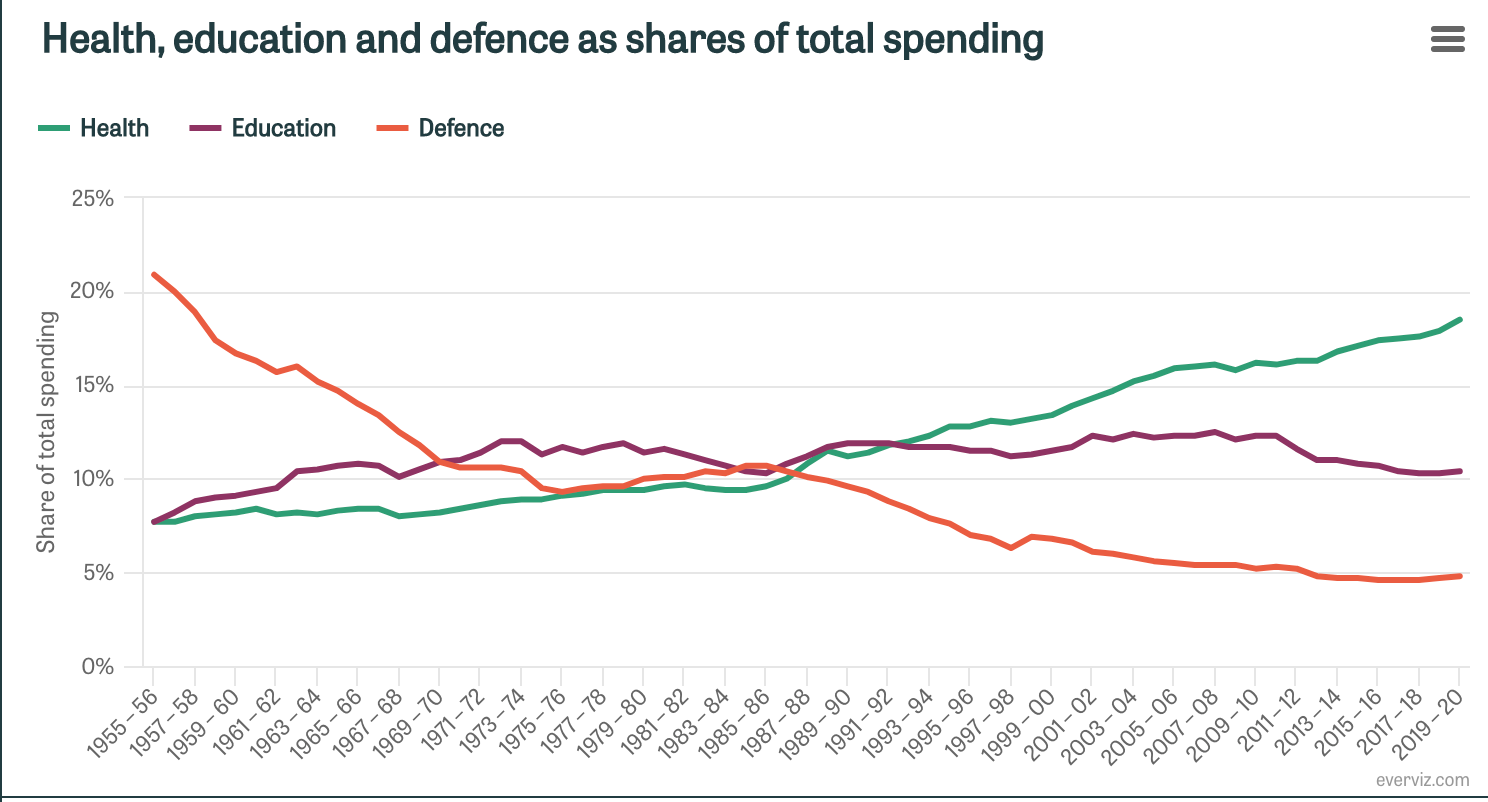
\includegraphics[width=4in]{images/ch3/4.png}
                \caption{Health, education and defence as shares of total spending}
                \label{fig:label}
            \end{figure} 
\begin{itemize}           
        \item Health spending takes a bigger share of total UK spending over the last 70 years.
        \item The share of education spending is approximately flat, and the share of defence spending declines significantly.
        \end{itemize}
        
        \subsection{Components of UK government spending}  
            \begin{figure}[H]%option [H] means "strictly here"
                \centering
                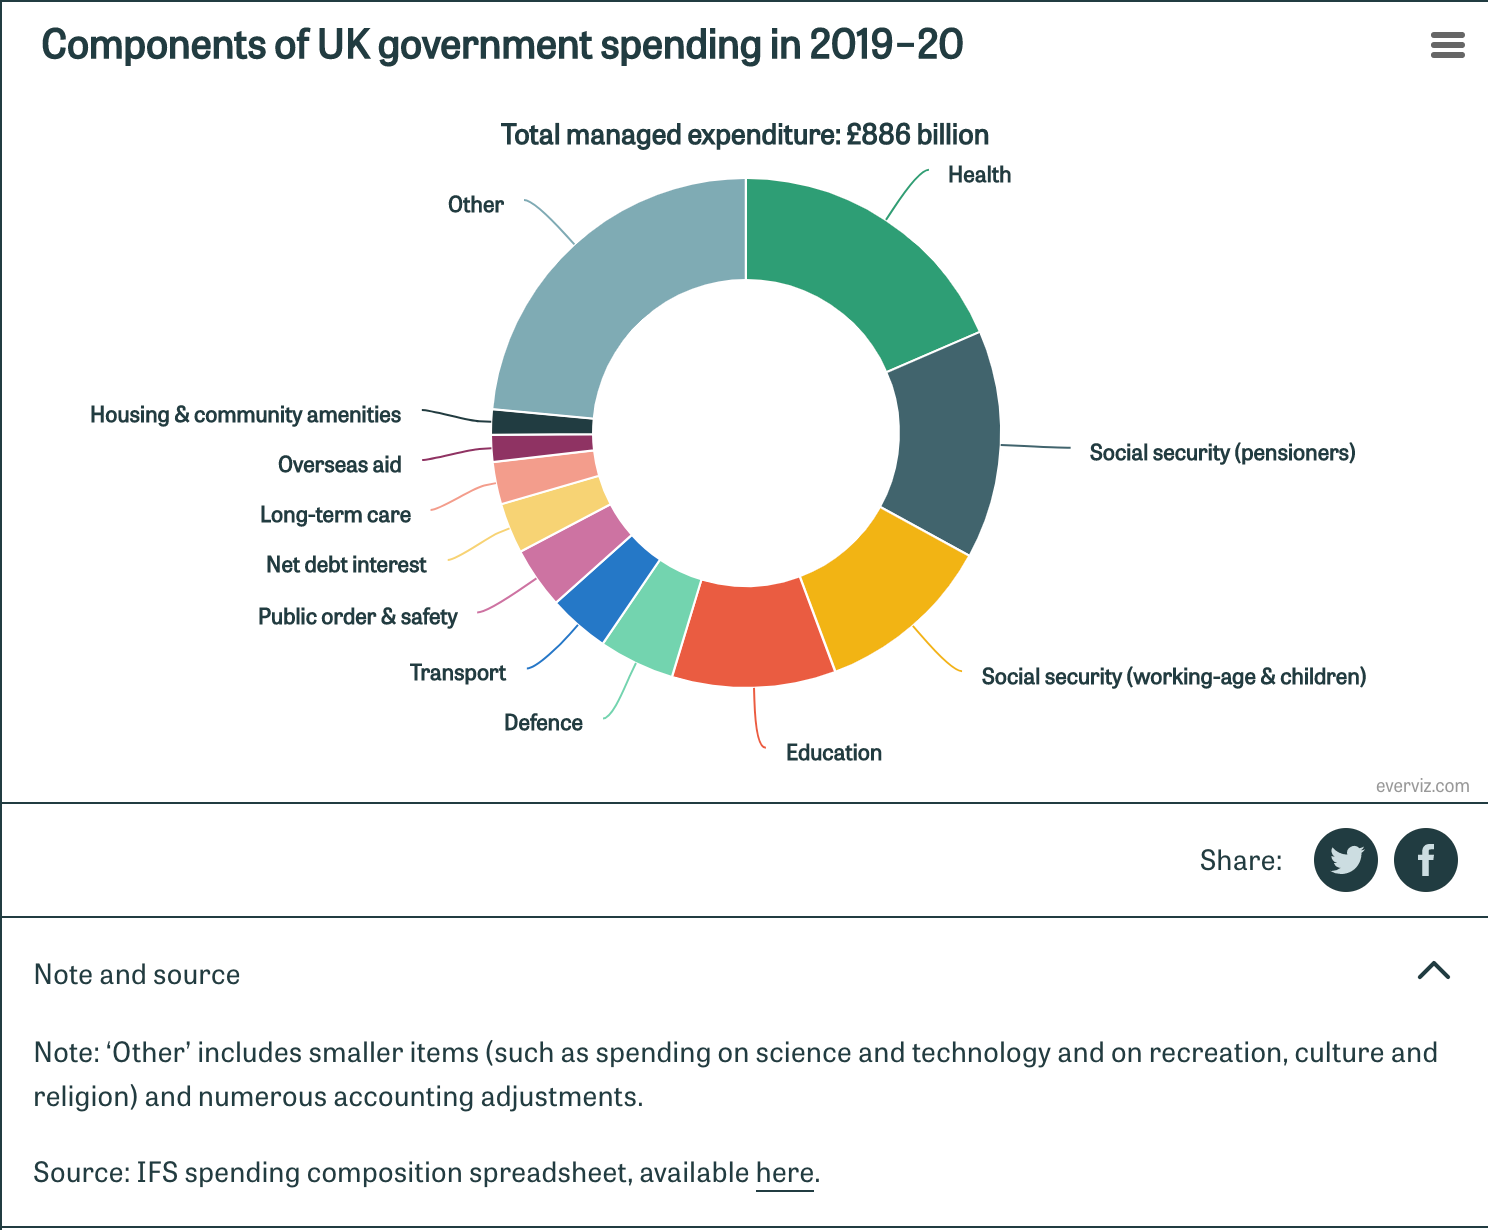
\includegraphics[width=4in]{images/ch3/5.png}
                \caption{Components of UK GOV spending in 2019-20}
                \label{fig:label}
            \end{figure} 
\begin{itemize}           
        \item Total managed UK government expenditure is 886 billion pounds, and health spending is a very important component.
        \end{itemize}

        \subsection{UK public spending on health}         
        \begin{figure}[H]%option [H] means "strictly here"
                \centering
                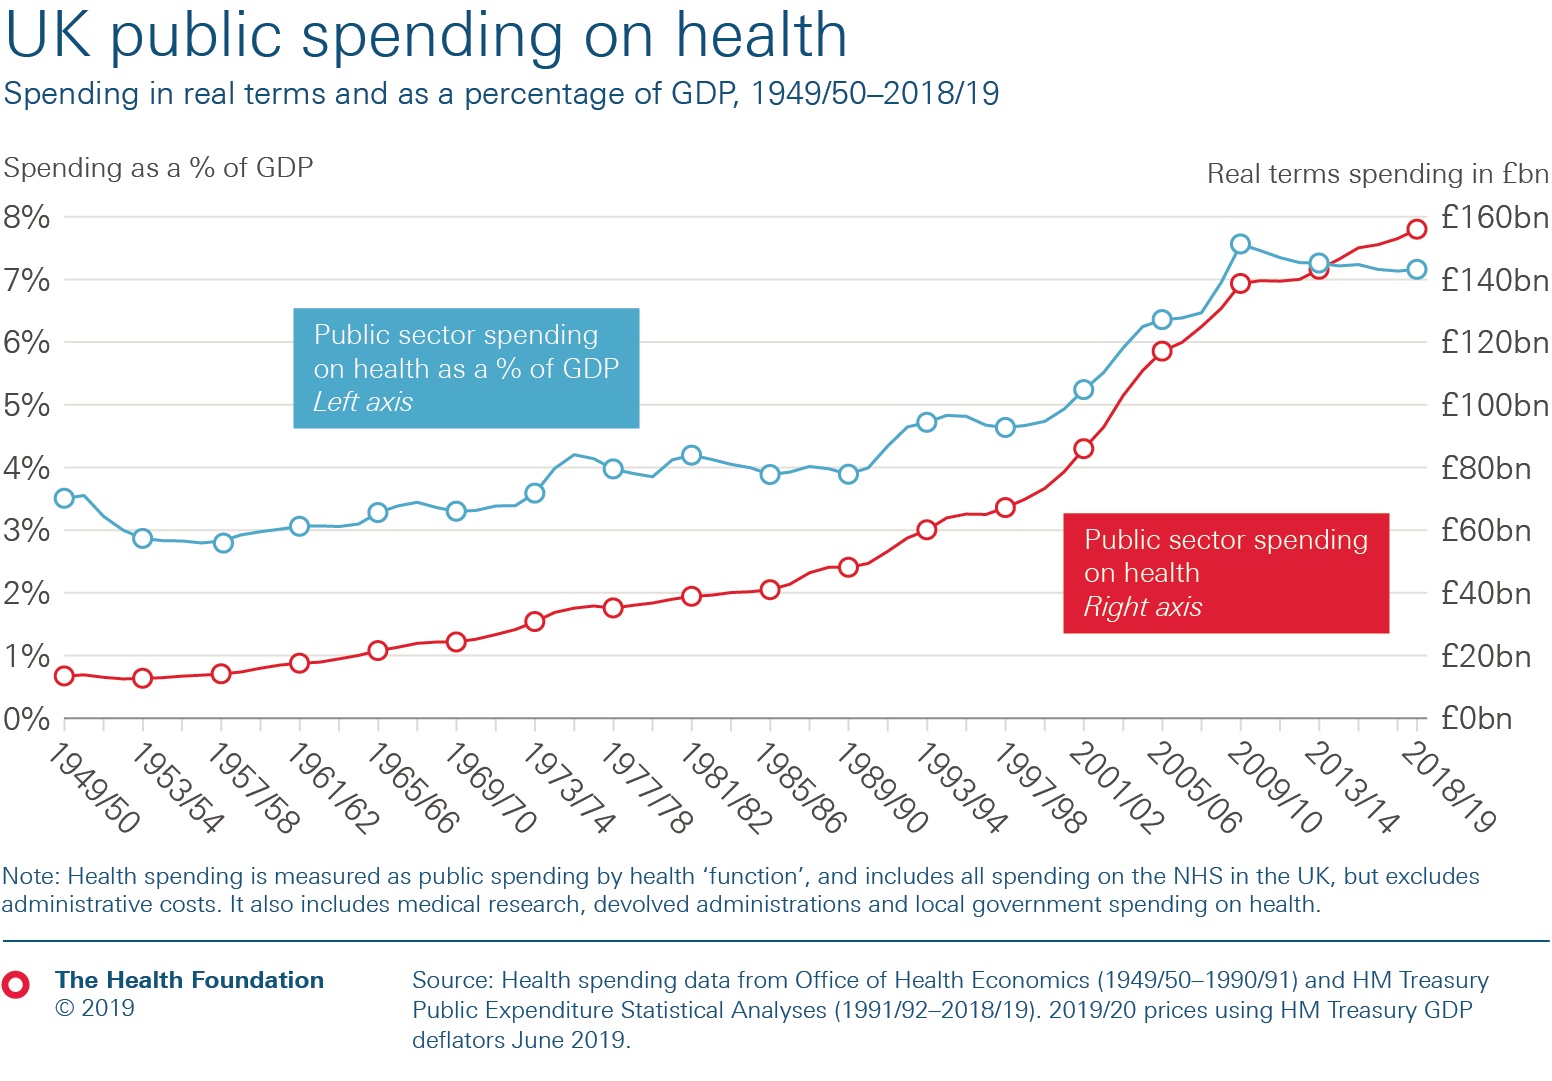
\includegraphics[width=4in]{images/ch3/6.png}
                \caption{UK public spending on health, 1949/50 - 2018/19}
                \label{fig:label}
            \end{figure} 
\begin{itemize}           
        \item The blue line shows the UK public sector spending on health as a percentage of GDP (left axis). The red line shows the UK public sector spending on health in real terms (right axis).
        \item The UK public sector spending on health has increased both as a percentage of GDP and in real terms since the end of World War II.
        \end{itemize}

        \subsection{Department of Health and Social Care spending} 
        \begin{figure}[H]%option [H] means "strictly here"
                \centering
                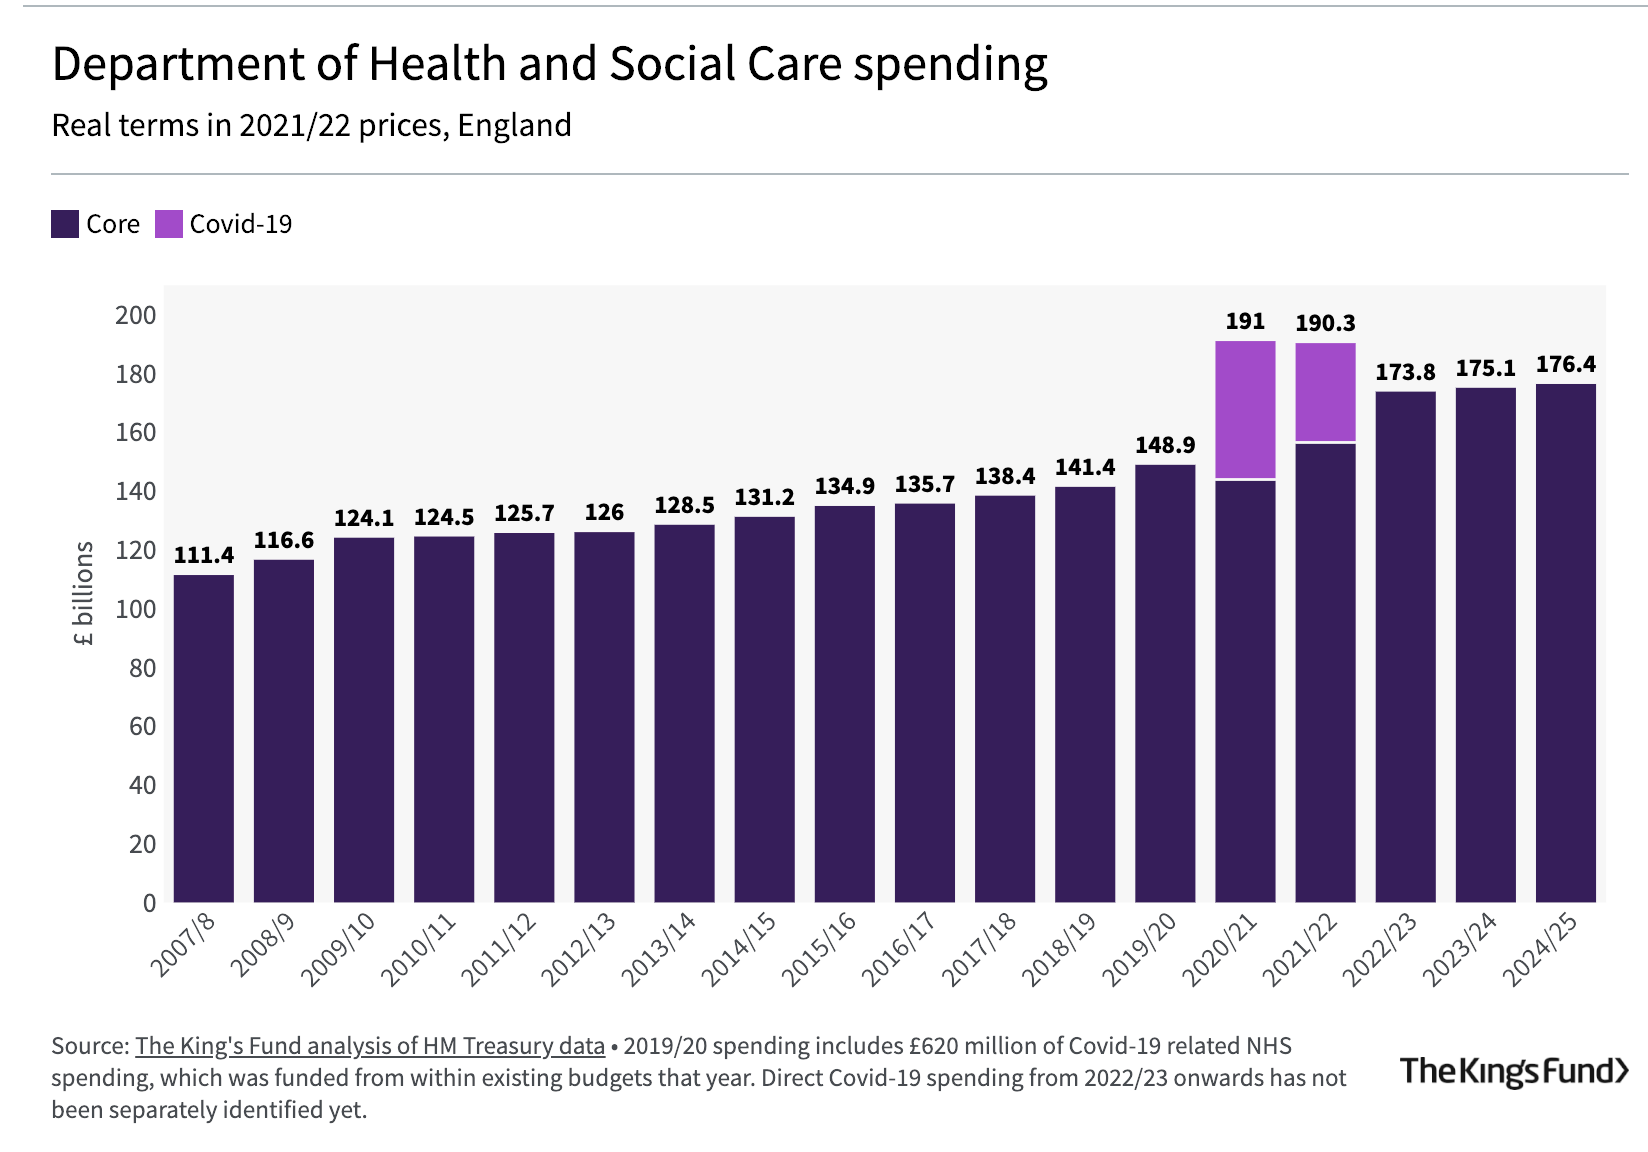
\includegraphics[width=4in]{images/ch3/7.png}
                \caption{Department of Health and Social Care spending, real terms in 2021/22 prices, England}
                \label{fig:label}
            \end{figure} 
\begin{itemize}           
        \item The Department of Health and Social Care spending increased a lot due to Covid-19, and the core spending keeps going up after 2021/22.
        \end{itemize}        

        \subsection{UK health spending growth} 
        \begin{figure}[H]%option [H] means "strictly here"
                \centering
                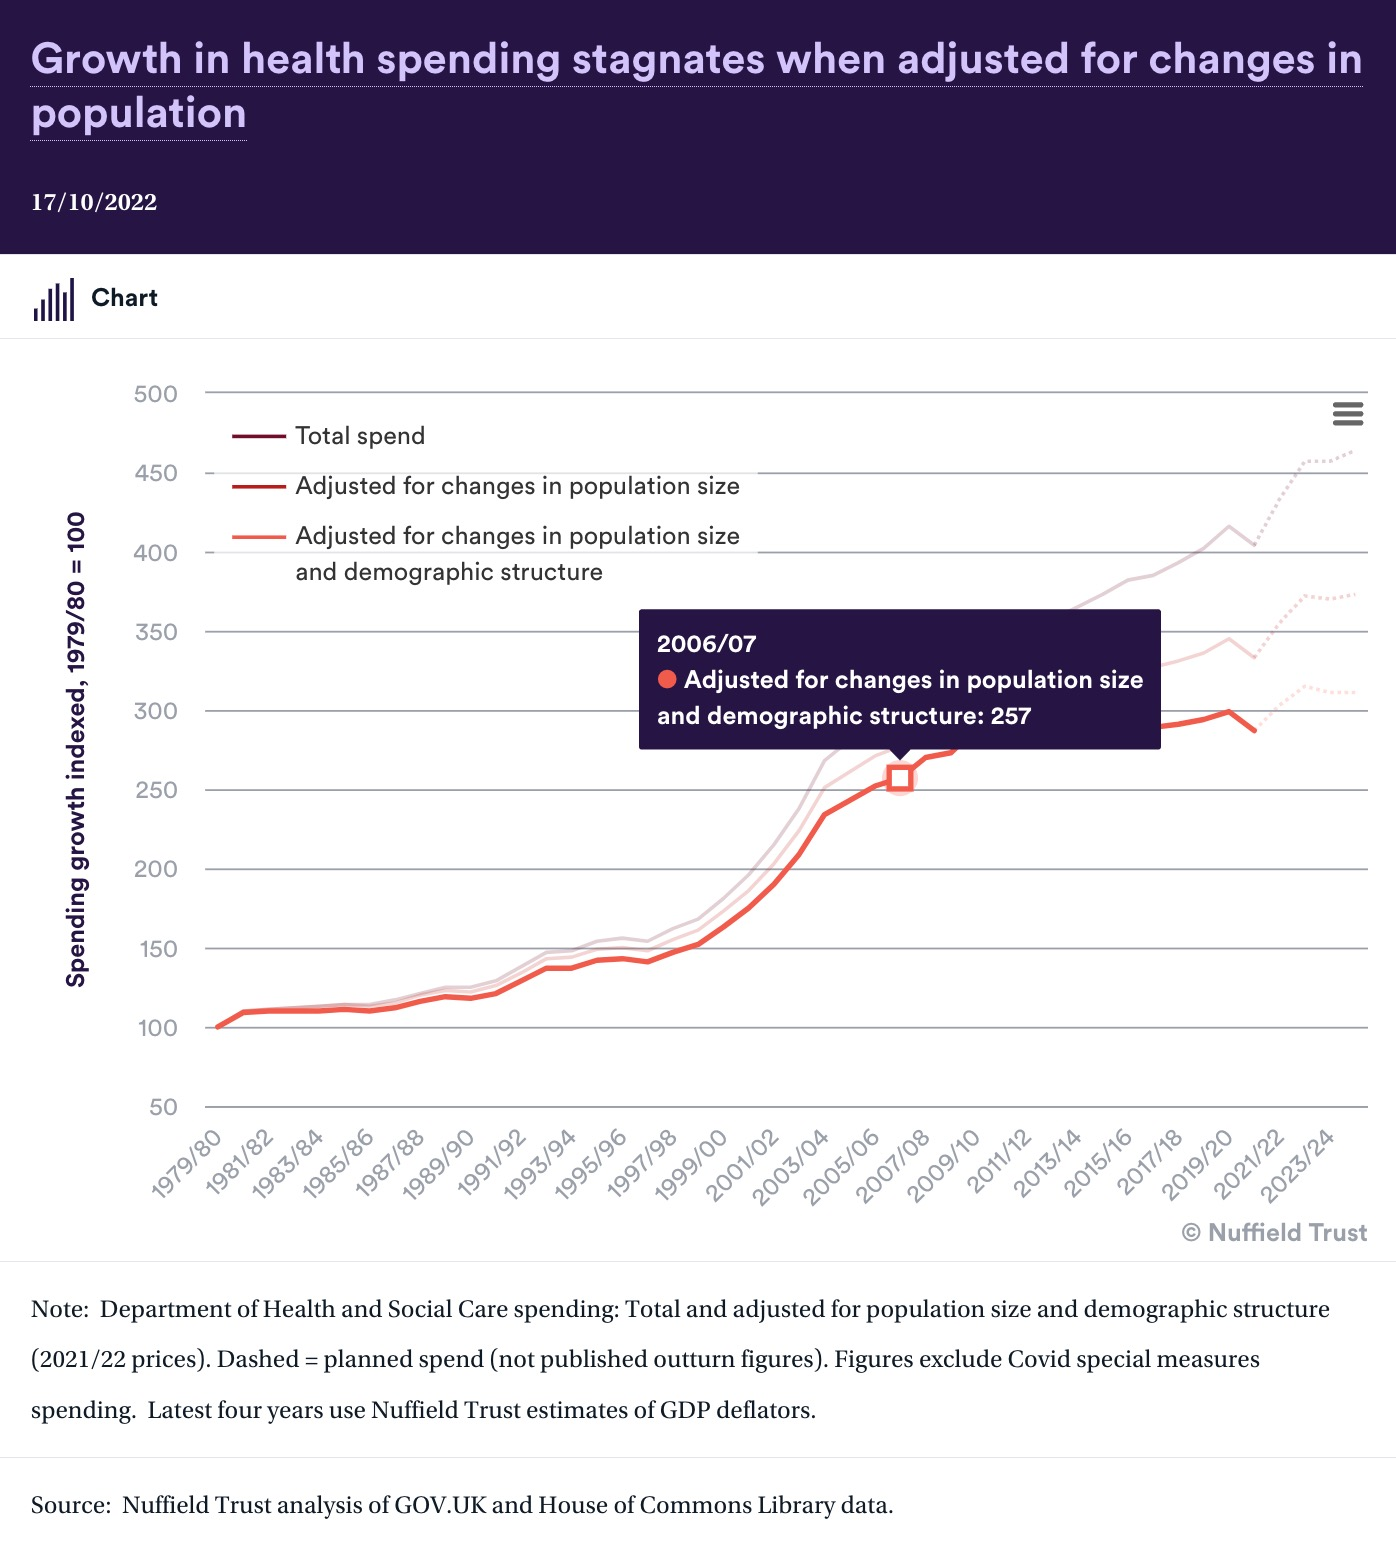
\includegraphics[width=4in]{images/ch3/8.png}
                \caption{Health spending growth indexed, 1979/80 = 100}
                \label{fig:label}
            \end{figure} 
\begin{itemize}           
        \item The dark red line shows the total health spending. The red line shows the total health spending adjusted for changes in population size. The orange line shows the total health spending adjusted for changes in population size and demographic structure.
        \item Growth in health spending stagnates when adjusted for changes in population (population ageing).
        \end{itemize}       

 \begin{figure}[H]%option [H] means "strictly here"
                \centering
                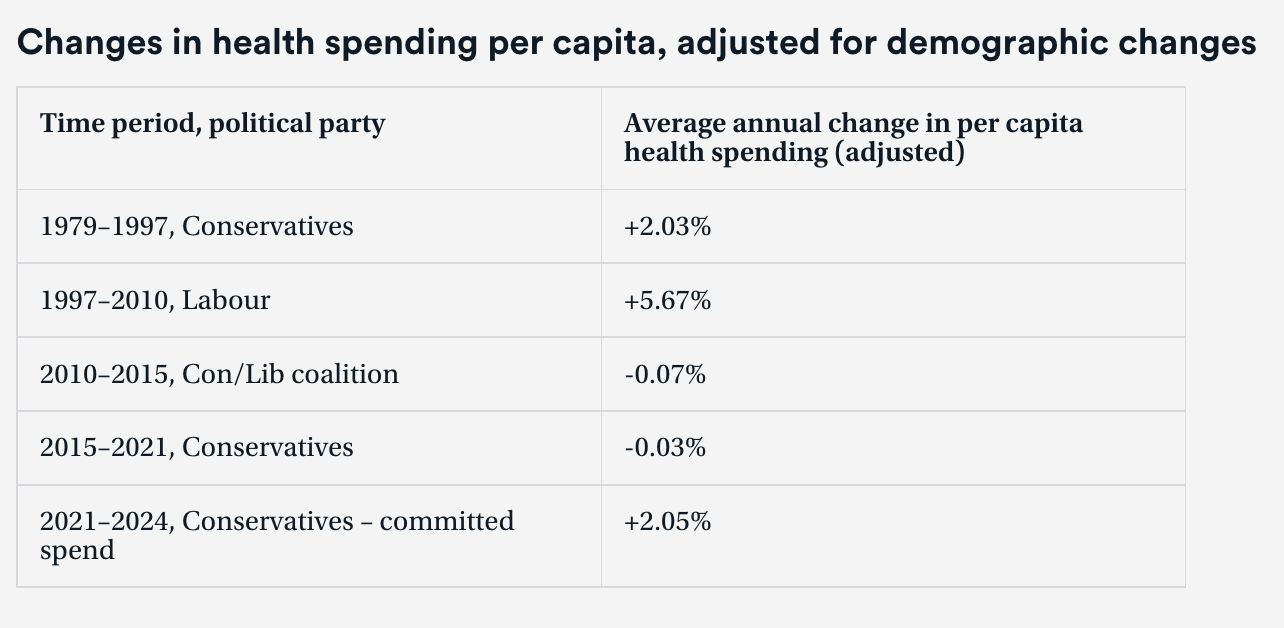
\includegraphics[width=4in]{images/ch3/9.png}
                \caption{Changes in health spending per capita, adjusted for demographic changes}
                \label{fig:label}
            \end{figure} 
\begin{itemize}           
        \item The Labour government has the highest increase in health spending per capita.
        \end{itemize}  
          
        \subsection{How funding flows in the NHS?} 
        \begin{figure}[H]%option [H] means "strictly here"
                \centering
                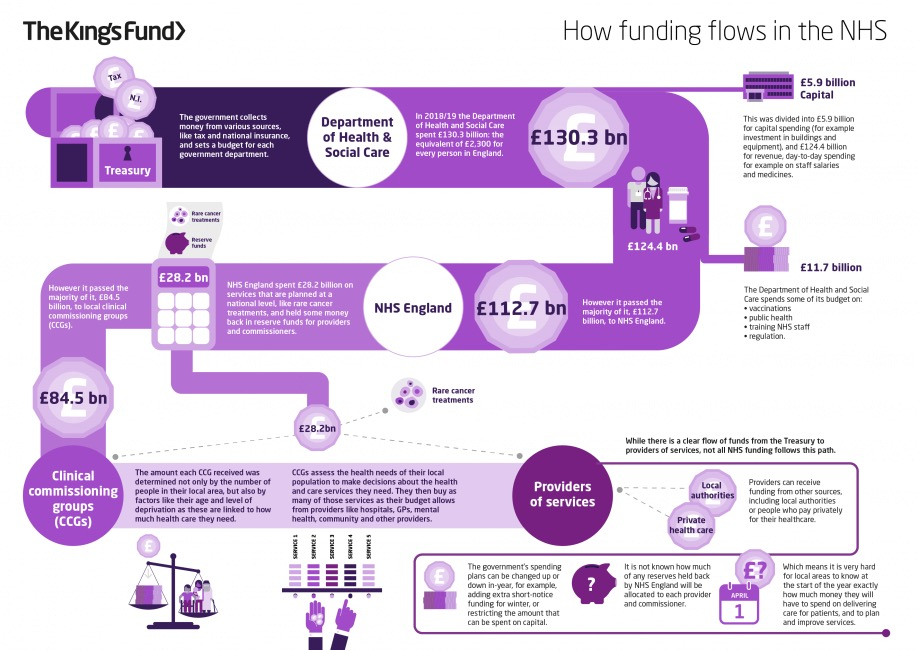
\includegraphics[width=5in]{images/ch3/11.png}
                \caption{How funding flows in the NHS?}
                \label{fig:label}
            \end{figure} 
\begin{itemize}           
        \item In 2018/19, the Treasury gave the Department of Health and Social Care 130.3 billion pounds. This was divided into 5.9 billion for capital spending and 124.4 billion for day-to-day spending. 
        \item The 124.4 billion was further divided into 11.7 billion for preventive services (vaccinations, public health, training NHS staff, and regulation) and 112.7 billion for NHS England. 
        \item NHS England spent 28.2 billion on national-planned services, such as rare cancer treatments, and passed the remaining 84.5 billion to the clinical commissioning groups (CCGs). The amount each CCG received was determined by the number of people in the local area and by factors such as age (how sick they are).
        \end{itemize} 

        \subsubsection{Example: Bradford CCG}         
        \begin{figure}[H]%option [H] means "strictly here"
                \centering
                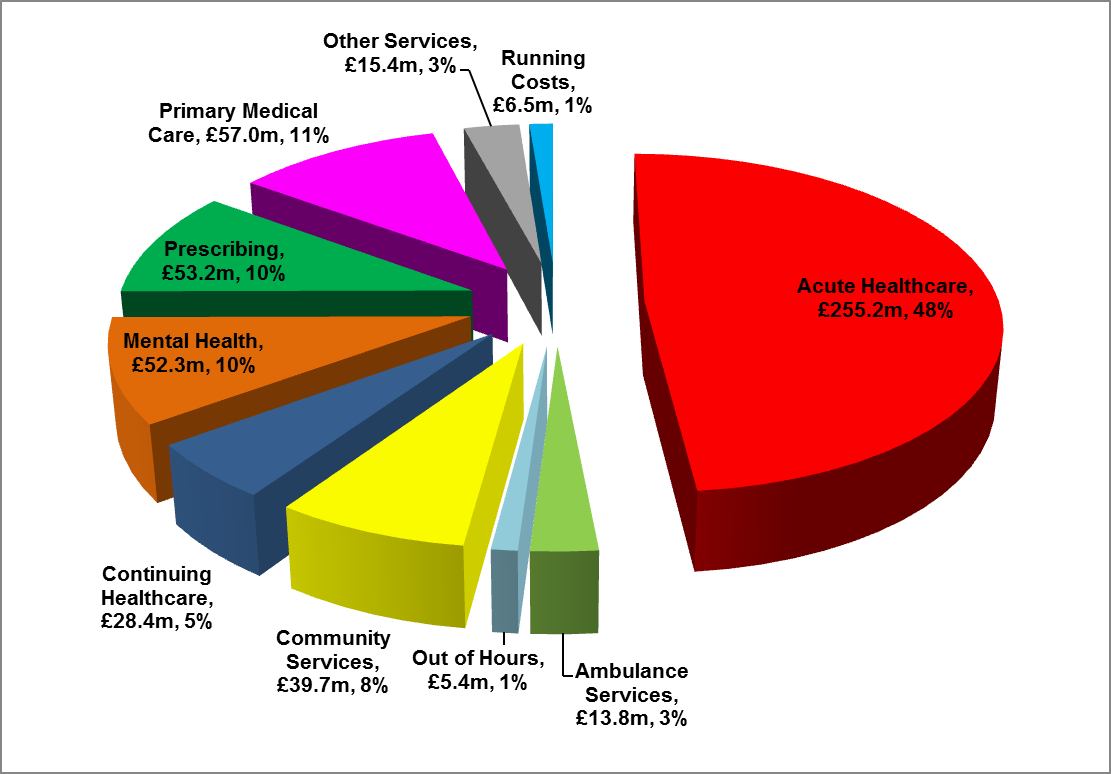
\includegraphics[width=4in]{images/ch3/12.png}
                \caption{Total CCG net expenditure, 2019/20(526.9 million pounds)}
                \label{fig:label}
            \end{figure} 
\begin{itemize}           
        \item Half of the money goes to acute healthcare. A small proportion of the money goes to preventive services, such as community services (health visitors and immunisation).
        \end{itemize}
        \begin{figure}[H]%option [H] means "strictly here"
                \centering
                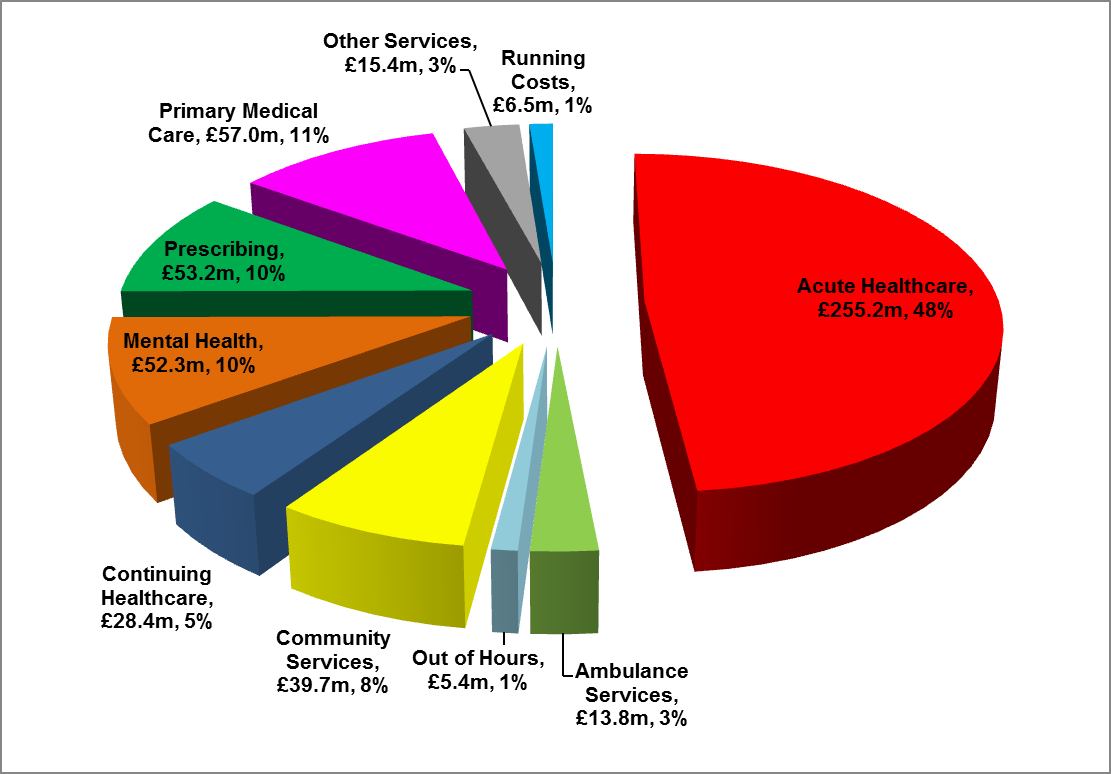
\includegraphics[width=4in]{images/ch3/13.png}
                \caption{Acute health expenditure}
                \label{fig:label}
            \end{figure}
\begin{itemize}           
        \item This graph shows the hospitals to which the acute healthcare expenditure goes.
        \end{itemize}

         \subsection{There are other factors that matter to health other than healthcare} 
        \begin{figure}[H]%option [H] means "strictly here"
                \centering
                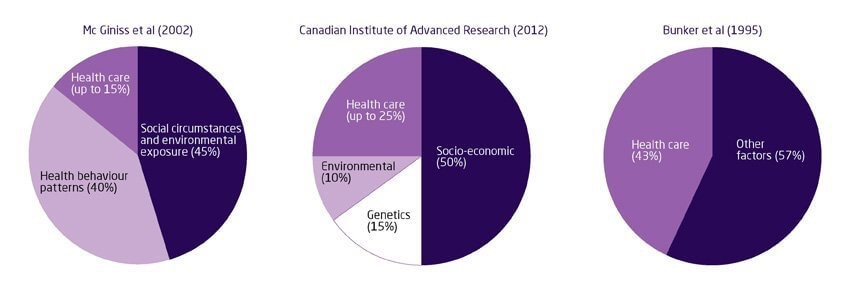
\includegraphics[width=5in]{images/ch3/14.png}
                \caption{There is more to health than healthcare}
                \label{fig:label}
            \end{figure} 
\begin{itemize}           
        \item  These three pie charts show the proportion of health that does not depend on the healthcare. Although the proportion varies between different studies, healthcare matters by less than a half in all studies.
        \end{itemize}


        \subsubsection{Example: The role of lifestyles in the prevention of chronic conditions}         
        \begin{figure}[H]%option [H] means "strictly here"
                \centering
                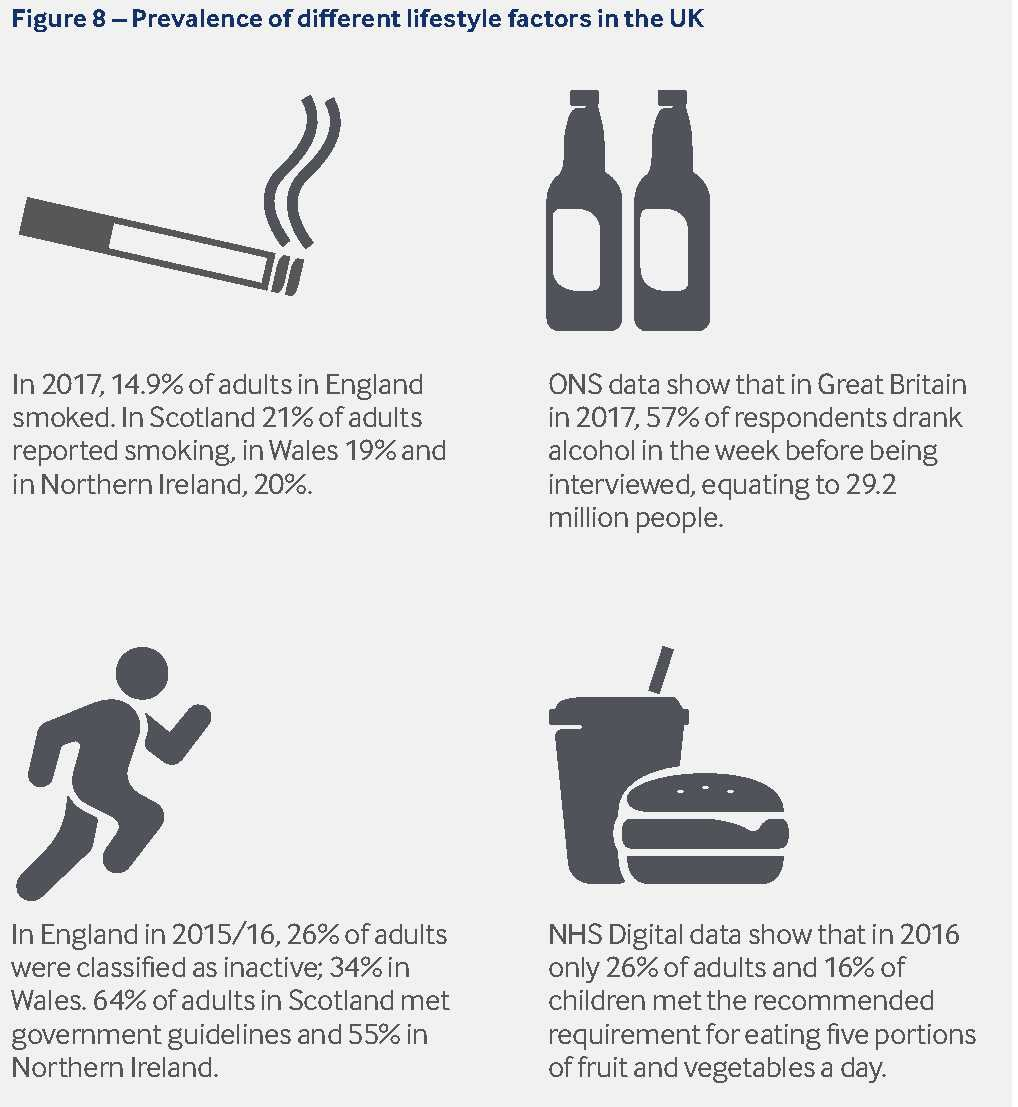
\includegraphics[width=3in]{images/ch3/15.png}
                \caption{Prevalence of different lifestyle factors in the UK}
                \label{fig:label}
            \end{figure} 
        \begin{figure}[H]%option [H] means "strictly here"
                \centering
                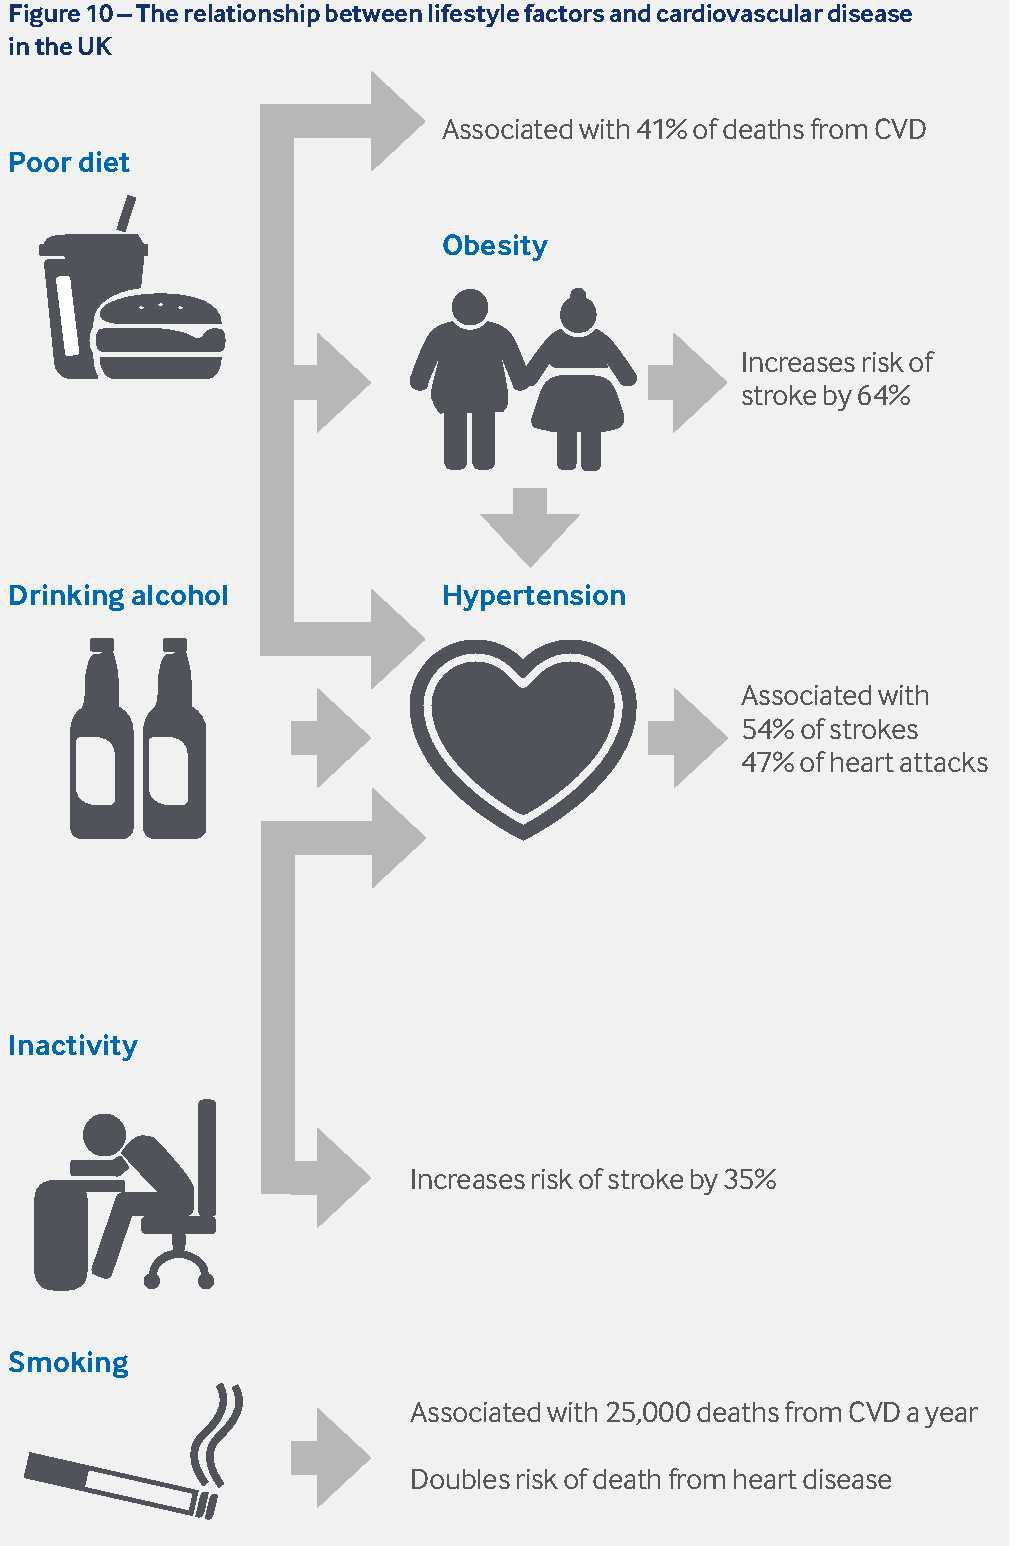
\includegraphics[width=3in]{images/ch3/16.png}
                \caption{The relationship between different lifestyle factors and cardiovascular diseases in the UK}
                \label{fig:label}
            \end{figure} 

\begin{itemize}           
        \item Poor lifestyles, such as poor diet, drinking alcohol, inactivity and smoking, are associated with cardiovascular diseases.
        \end{itemize}

\begin{figure}[H]%option [H] means "strictly here"
                \centering
                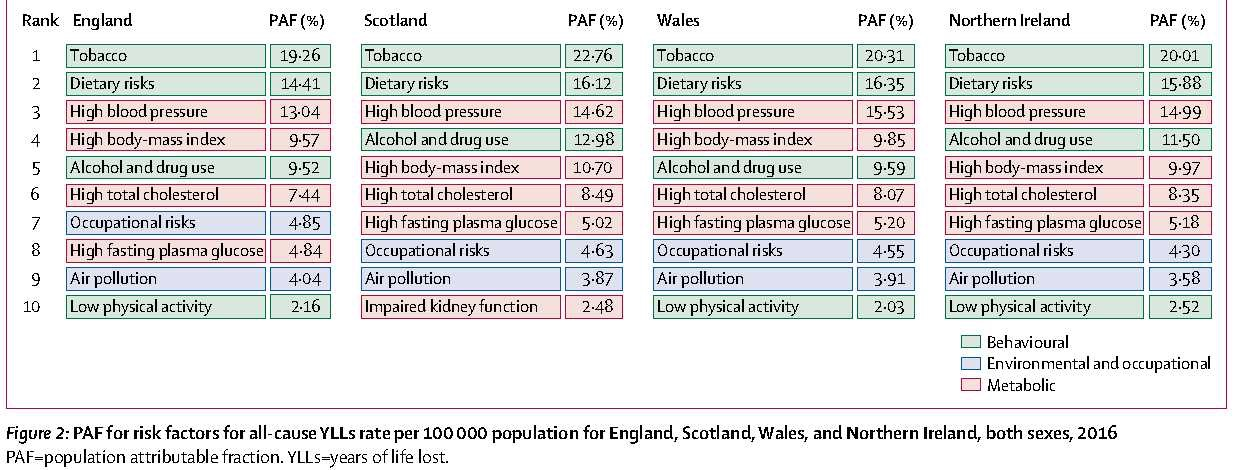
\includegraphics[width=5in]{images/ch3/17.png}
                \caption{PAF (Population Attributable Factions) for major risk factors for all-cause YLLs (Years of Life Lost) rate per 100 000 population for England, Scotland, Wales, and Northern Ireland, both sexes, 2016}
                \label{fig:label}
            \end{figure} 

\begin{itemize}           
        \item The population attributable fraction is the proportional reduction in population disease or mortality that would occur if exposure to a risk factor were reduced to an alternative ideal exposure scenario. 
        \item The ten leading risk factors contributing to YLLs were similar in rank across the four regions of the UK. Although the ranks were similar, the PAF of each risk factor varied in size in different countries, such as a higher PAF from tobacco in Scotland, and from alcohol and drug use in Scotland and Northern Ireland, compared with the other UK regions.
        \item Poor lifestyles do matter for health, although most money goes to curative health.
        \end{itemize}

        \subsection{How is the health budget spent?} 
        \subsubsection{Worldwide}
        \begin{figure}[H]%option [H] means "strictly here"
                \centering
                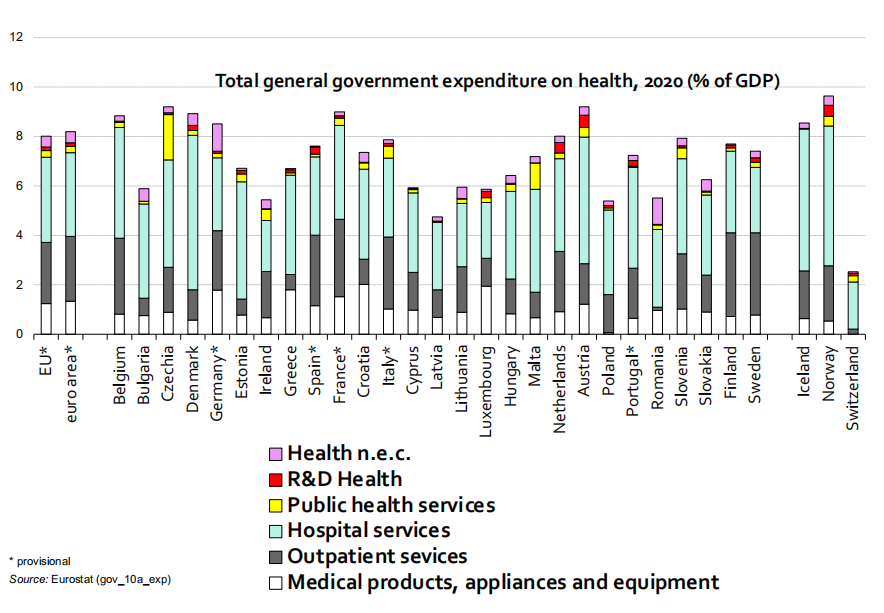
\includegraphics[width=4in]{images/ch3/10.png}
                \caption{Total general government expenditure on health as a percentage of GDP, 2020}
                \label{fig:label}
            \end{figure} 
\begin{itemize}           
        \item The biggest share goes to hospital services, followed by outpatient services, so most money is used to treat people in the first place.
        \end{itemize}
        
        \subsubsection{UK}
        \begin{figure}[H]%option [H] means "strictly here"
                \centering
                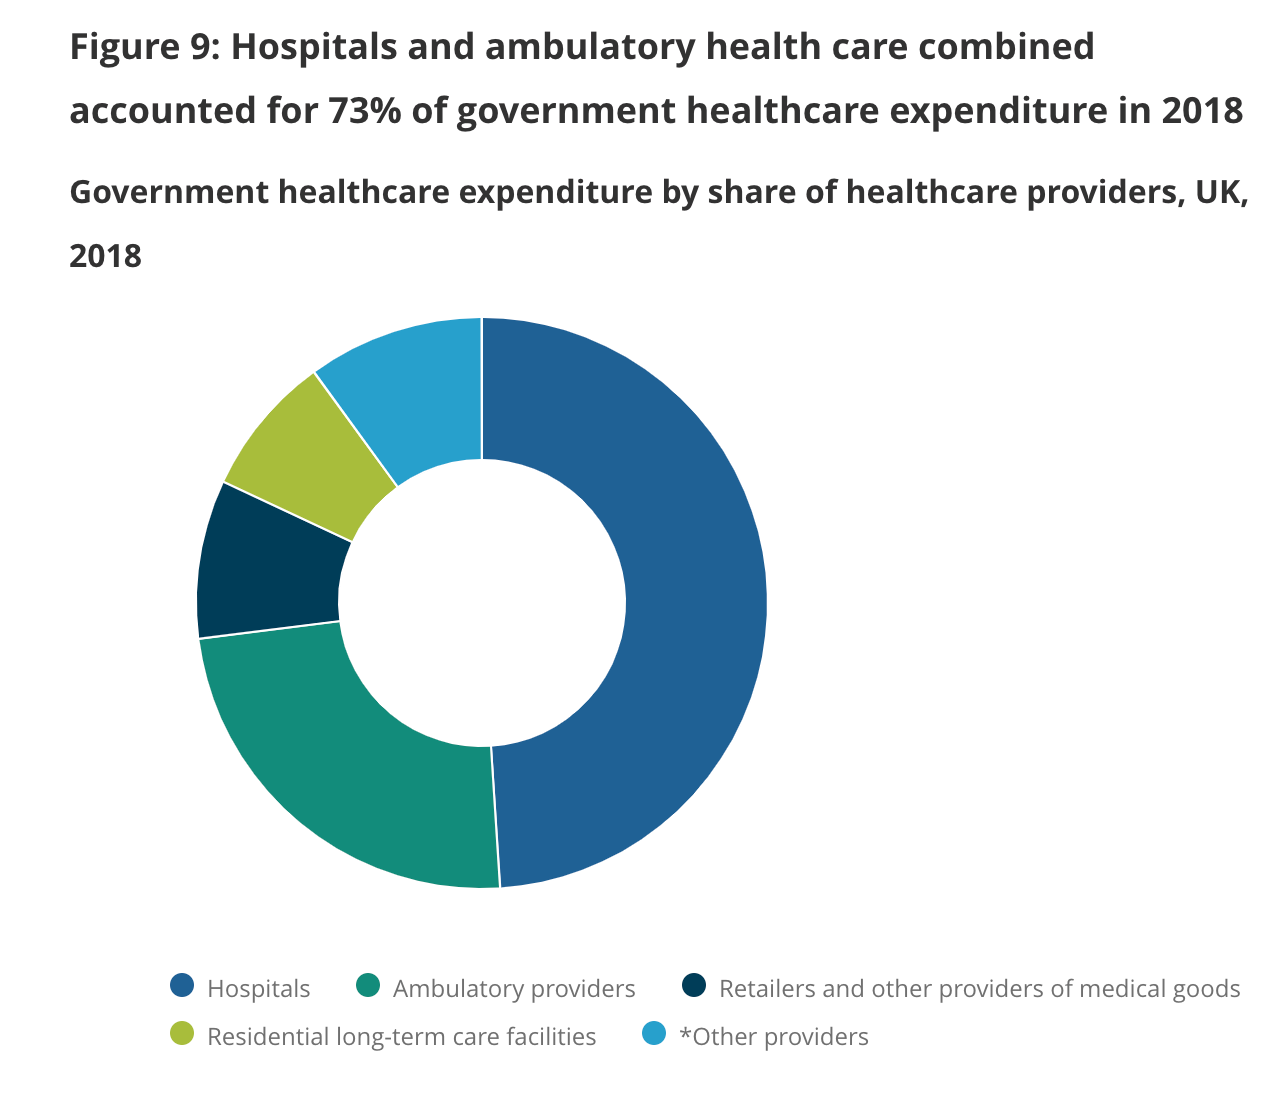
\includegraphics[width=4in]{images/ch3/18.png}
                \caption{Government healthcare expenditure by share of healthcare providers, UK, 2018}
                \label{fig:label}
            \end{figure} 
 \begin{itemize}           
        \item Hospitals and ambulatory healthcare combined accounted for 73 percent of government healthcare expenditure in 2018
        \end{itemize}              

\subsubsection{Preventive care expenditure is easy to cut, UK}
        \begin{figure}[H]%option [H] means "strictly here"
                \centering
                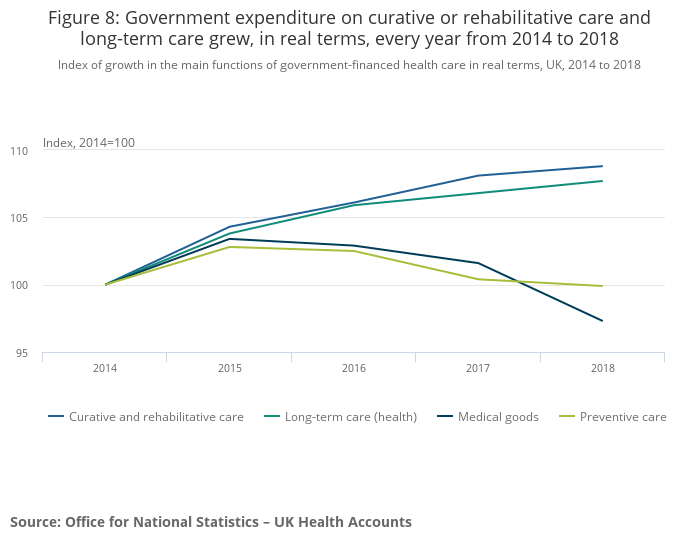
\includegraphics[width=4in]{images/ch3/19.png}
                \caption{Government expenditure on curative or rehabilitative care and long-term care grew, in real terms, every year from 2014 to 2018, index: 2014 = 100}
                \label{fig:label}
            \end{figure}
\begin{itemize}           
        \item Preventive care expenditure has decreased since 2015. This is because it is easy to cut. Curative care is difficult to cut, so the expenditure has increased over time.
        \end{itemize} 

        \begin{figure}[H]%option [H] means "strictly here"
                \centering
                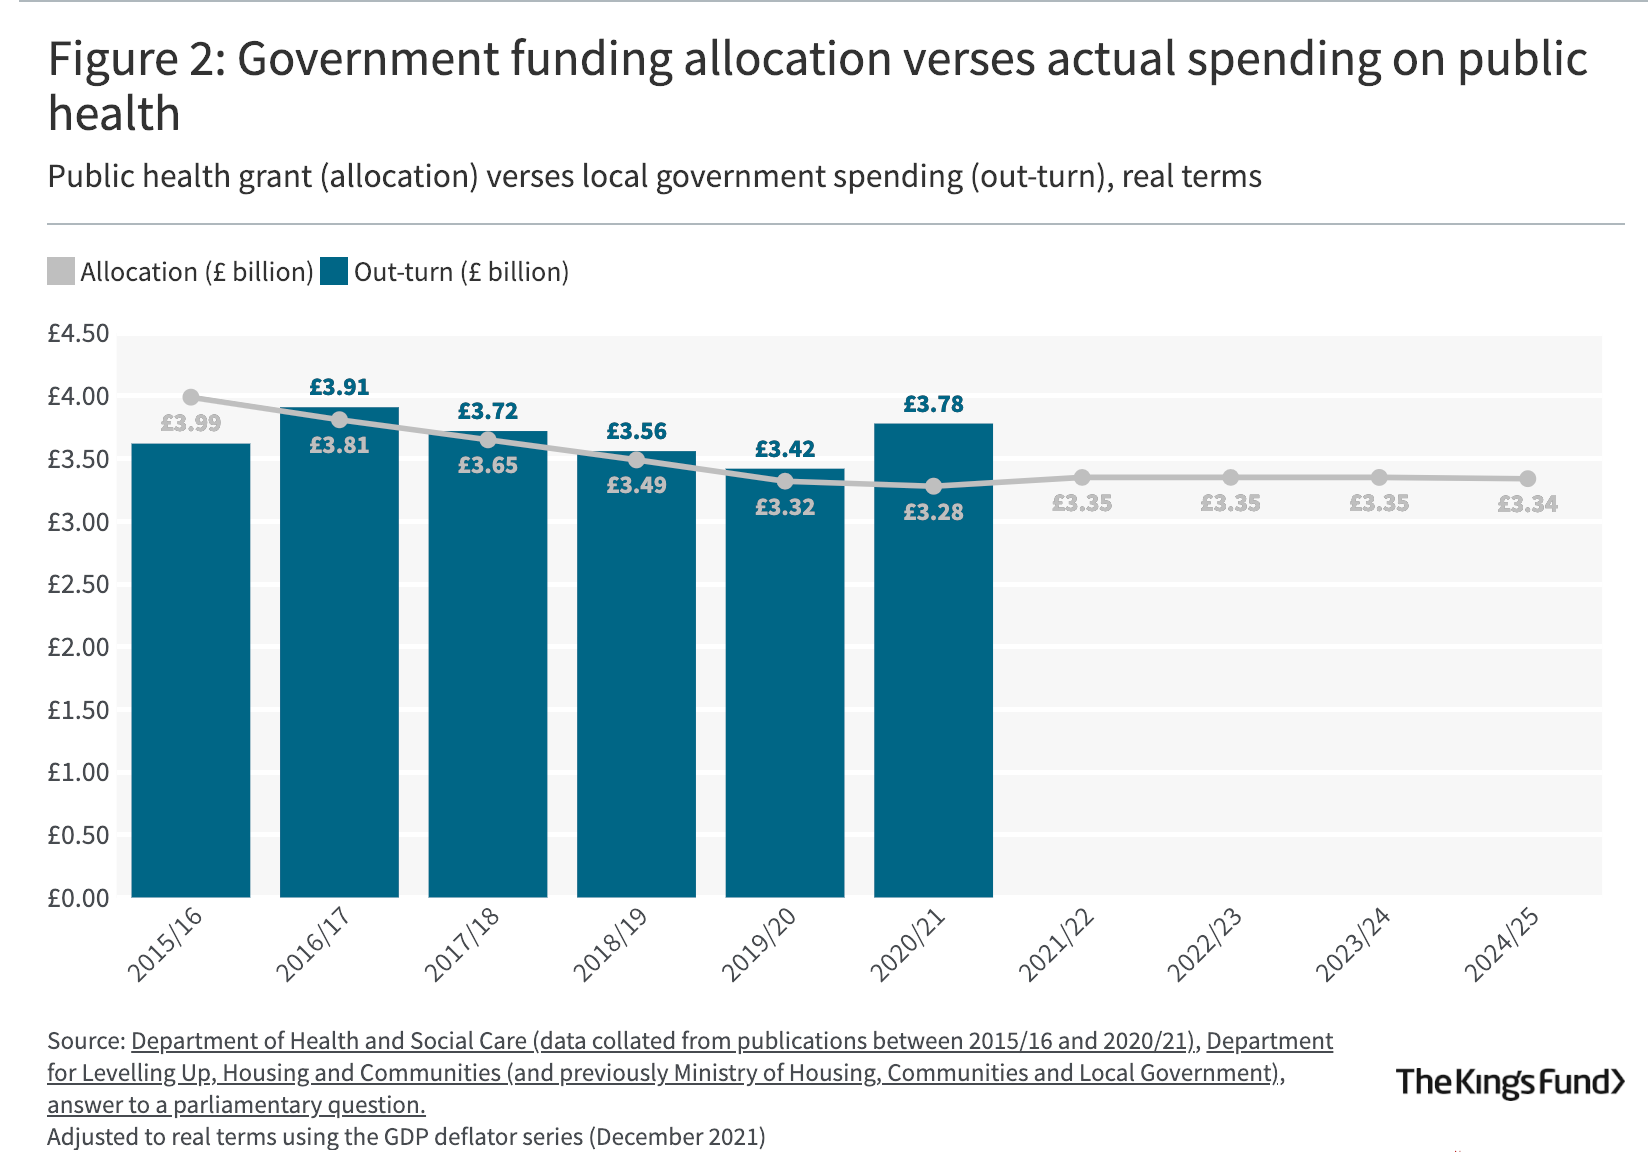
\includegraphics[width=4in]{images/ch3/20.png}
                \caption{Public health grant (allocation) VS local government spending (out-turn), real terms}
                \label{fig:label}
            \end{figure}
\begin{itemize}           
        \item The blue bars show the total local government spending on healthcare, which increased in 2020/21 due to Covid-19.
        \item The grey line shows the money allocated to public health prevention. It decreased since 2015/16. This is because it is easy to cut. 
        \end{itemize} 
        
        \begin{figure}[H]%option [H] means "strictly here"
                \centering
                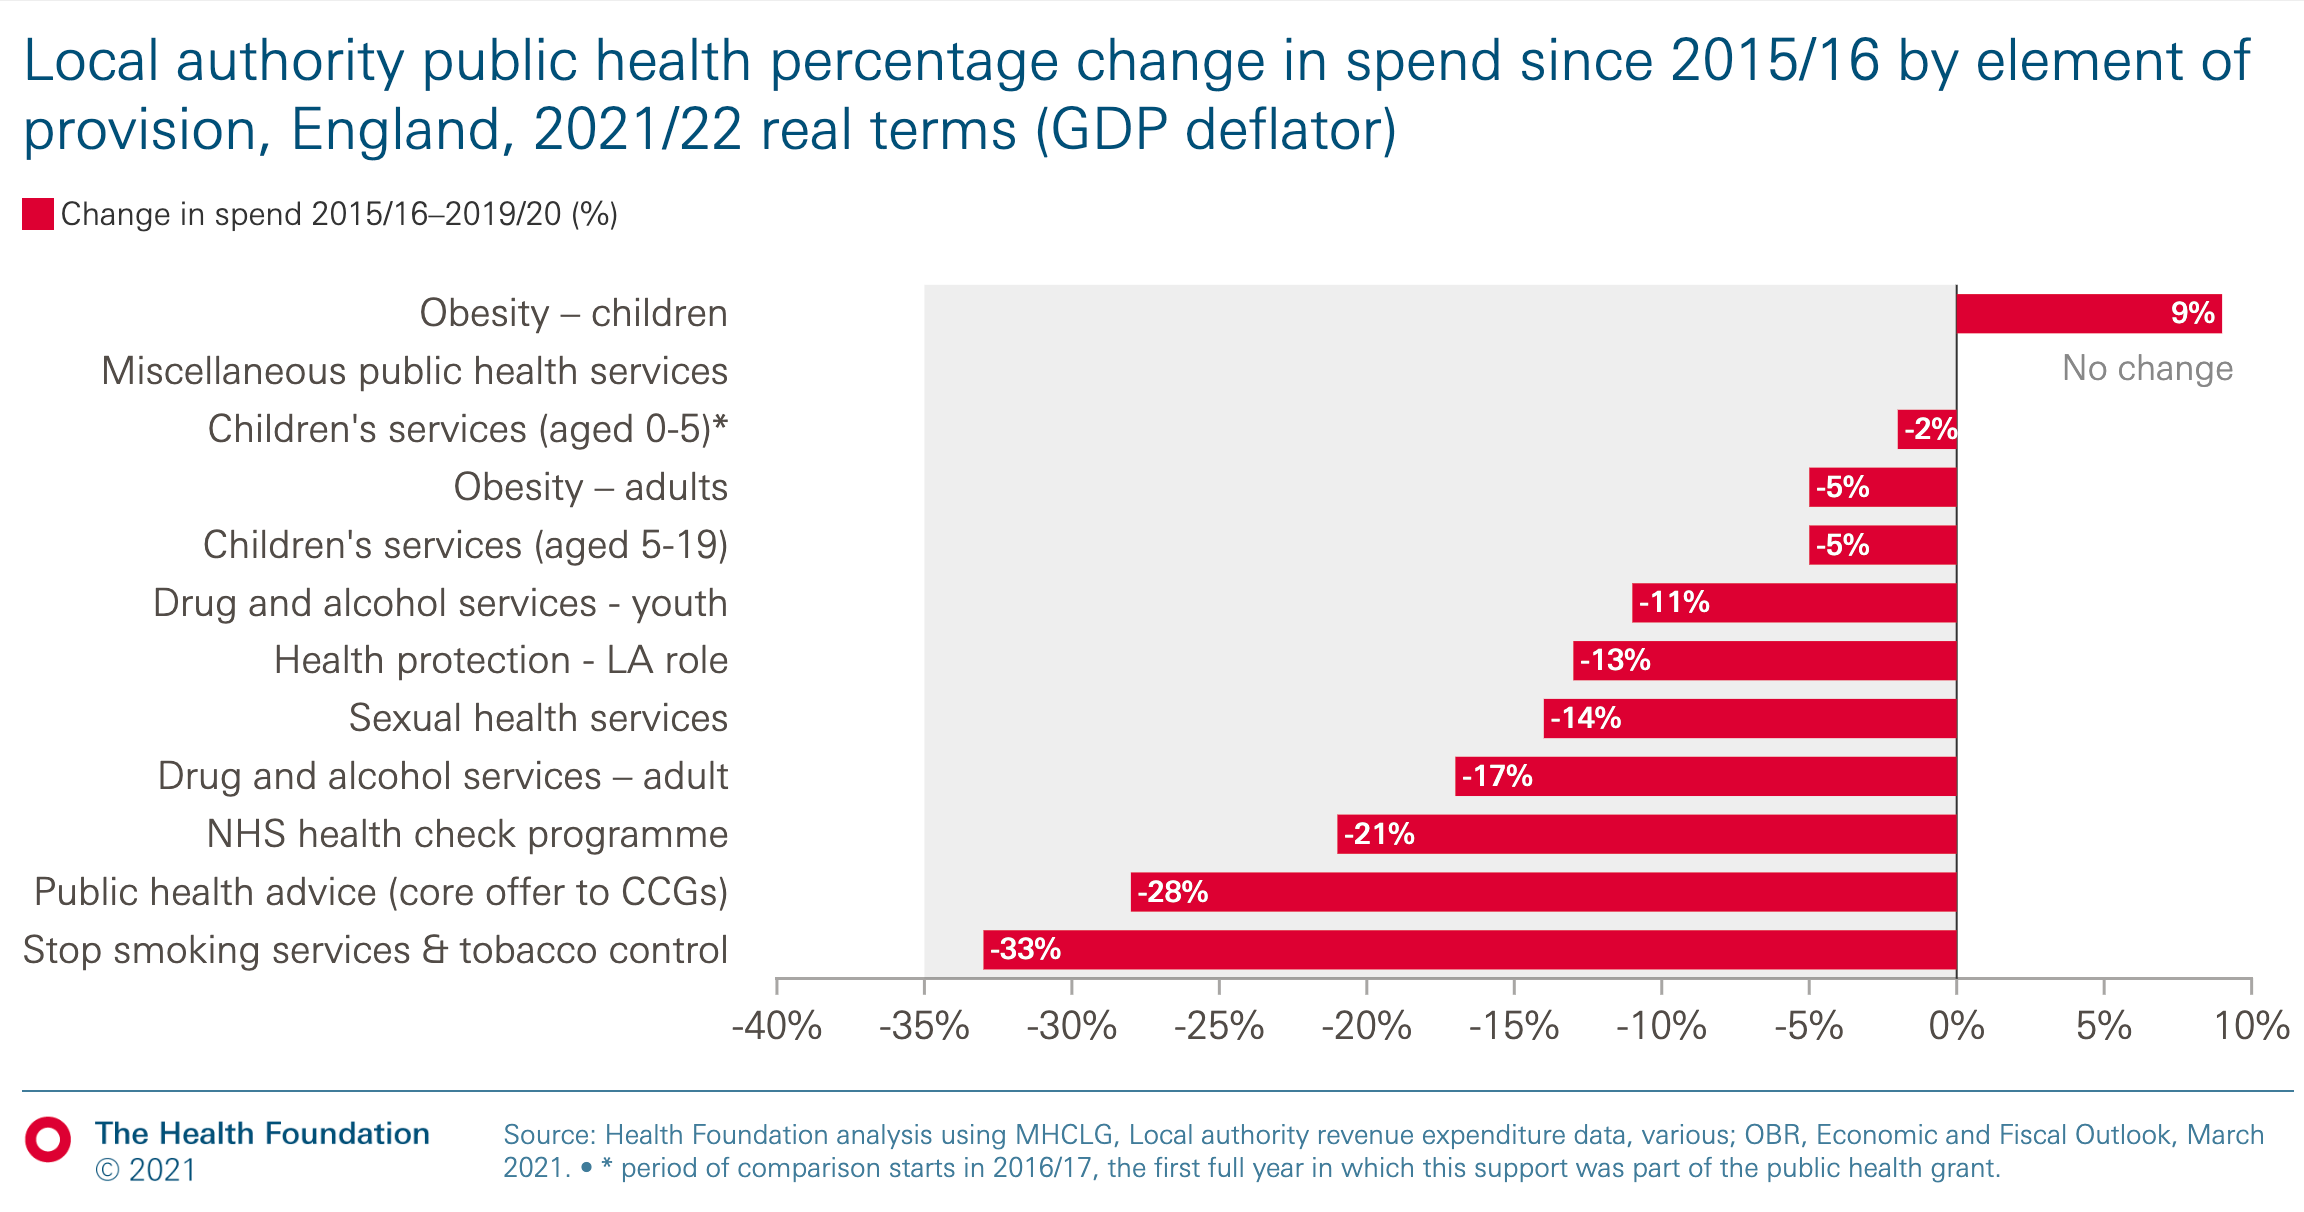
\includegraphics[width=4in]{images/ch3/21.png}
                \caption{Local authority public health percentage change in spending since 2015/16 by element of provision, England, 2021/22 real terms (GDP deflator)}
                \label{fig:label}
            \end{figure}
\begin{itemize}           
        \item For preventive healthcare expenditure, only obesity for children increased, since it is a major problem for children in the UK and costs NHS a lot of money. The expenditure is cut across all other categories.
        \end{itemize} 

        \subsection{Early Intervention and Prevention}
\begin{itemize}           
        \item Early intervention and prevention approaches aim to support health and wellbeing by taking action before health problems worsen, or by preventing health problems for occurring in the first place. 
        \item Public Health Prevention = improving public health through disease prevention
        a. Clinical interventions such as screening and vaccinations;
        b. Population-level measures aimed at influencing health behaviours or
addressing the social determinants of health (e.g. living conditions, education etc.).
        \item Early Intervention = strategies aimed to mitigate the effects of problems once they have been identified.
        – Some specifically targeted at the ‘early years’, including pregnancy, early parenting and the early parent-child relationship.
        \item A NICE (National Institute for Health and Care Excellence) review of the cost-effectiveness of 200 interventions found that 30 (15 percent) were cost-saving and 141 (70.5 percent) were cost-effective.
        \end{itemize} 

\subsection{Why government intervention in getting people to become healthier?}
        \begin{figure}[H]%option [H] means "strictly here"
                \centering
                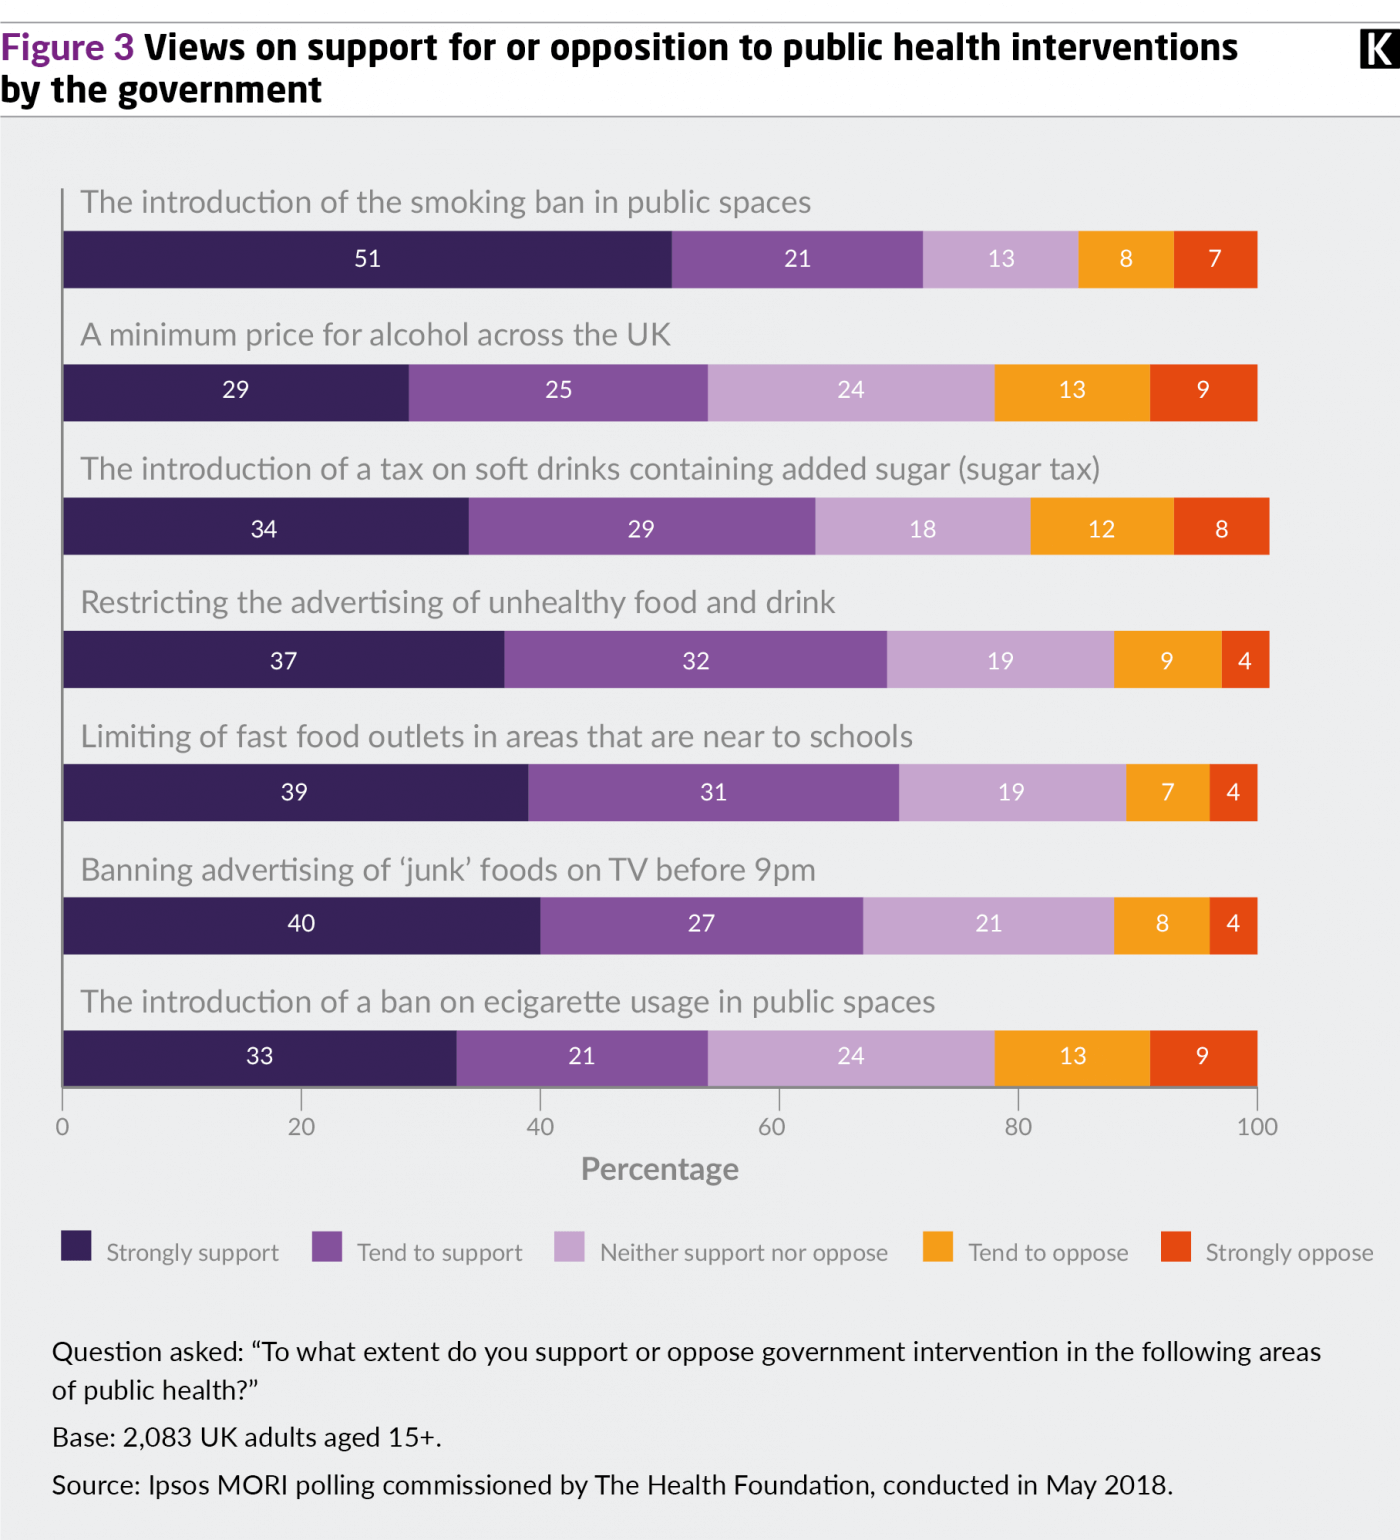
\includegraphics[width=4in]{images/ch3/22.png}
                \caption{Views on support for or opposition to public health interventions by the government}
                \label{fig:label}
            \end{figure}

\subsubsection{Reasons for government intervention:}          
\begin{itemize}           
        \item improve human capital, increase productivity, raise tax revenue in the future
        \item market failure: asymmetric information (e.g. junk food: consumers don't know the content/how much is going to harm them)
        \item public goods: hospital/public health services, nobody provides unless the government provides, it is expensive
        \item moral hazards
        \item negative externality (smoking)
        \item time-inconsistent preference (procrastination: go to the gym); addictive goods - the government can nudge/remind people
        \item In order to make progress and develop effective policies, we need first to understand how health is produced.
\end{itemize} 

\section{The Production of Health as Human Capital: The Grossman Model}
\subsection{Introduction}
\begin{itemize}
        \item Grossman (1972) studied how individuals allocate their resources to produce health. He combined the theory of human capital and the theory of the allocation of time to explain the demand for health. Health is a different good. We use time/resources/money to produce it and enjoy it.
        \item Four important aspects
        \begin{enumerate}
                \item Health can be treated both as a consumption and an investment good. As a consumption good, health yields direct utility. As an investment good, health increases the number of healthy days available to participate in the market and non-market activities.
                \item Health lasts for more than one period. It depreciates (e.g. ageing process; if no vaccine immunity, poorer health; if don't go to the gym, poorer health) and can be analyzed like a capital good.
                \item Individuals are not passive consumers of health: they produce it, spending time and money (buy market inputs).
                \item Demand for medical care is derived: people demand medical care not per se, but to produce health.
            \end{enumerate}
        \item As both a consumption and an investment good, optimal health capital accumulation requires the decision-making of its owner – the individual – who is both the consumer and the producer.    
\end{itemize}        

\subsection{Preferences}
\begin{itemize}
        \item Health as a consumption good enters directly into utility.
        \item Intertemporal utility function: $$\color{red} U = U(\varphi_0 H_0,...,\varphi_0 H_n,Z_0,...,Z_n)$$  
        \begin{enumerate} 
        \item $H_0$ = inherited stock of health (predetermined)
        \item $H_i$ = stock of health in the ith time period
        \item $\varphi_i$ = service flow per unit stock
        \item $h_i$ = $\varphi_iH_i$ = healthy days
        \item $Z_i$ = non-health commodity
        \end{enumerate}
        \item Length of life is endogenous: death occurs when H = $H_{min}$
        \item Individual maximises utility subject to production and resource constraints.
\end{itemize}

\subsection{Resource Constraints}
\begin{itemize}
        \item Budget Constraint
        $$\color{red} \sum_{i=0}^n\frac{P_iM_i+V_iX_i}{(1+r)^i}=\sum_{i=0}^n\frac{W_iTW_i}{(1+r)^i}+ A_0$$
        \begin{enumerate} 
        \item $P_i$ = price for health and $V_i$ = price for non-health commodity
        \item $W_i$ = wage rate
        \item $TW_i$ = time spent working 
        \item $A_0$ = initial assets
        \item $M_i$ = good inputs in the production of health
        \item r = interest rate
        \item $X_i$ = good inputs in the non-health commodity
        \item present discount value of health and non-health commodity = present discount value of labour market earnings + initial assets
        \end{enumerate}
        \item Time Constraint
        $$\color{red} TW_i+TL_i+TH_i+T_i= \aleph $$
        \begin{enumerate}
        \item $TW_i$ = time spent on working
        \item $TL_i$ = time loss due to illness
        \item $TH_i$ = time spent on producing health
        \item $T_i$ = time spent on producing other goods we enjoy
        \item  $\aleph$  = overall time endowment
        \end{enumerate}
        $$\color{red} TL_i= \aleph - h_i $$
        \begin{enumerate}
        \item $h_i$ = healthy days
        \end{enumerate}
\end{itemize}    

\subsection{Production technologies}
\begin{itemize}
        \item Healthy Time Production $\color{red} h_i=f(H_i)$
        
        Health days can be produced by some technology using health stocks.
        
        \item Health Stock Production $\color{red} H_{i+1}=H_i-\delta_iH_i+I_i$
        \begin{enumerate}
        \item $I_i$ = gross investment
        \item $\delta_i$ = depreciation (exogenous, might vary with age, e.g. older, higher depreciation)
        \item When investment is high, it can overcome the high rate of depreciation
        \item Problem with linear specification: doesn't account for diminishing marginal returns of investment; doesn't account for random shocks
        \end{enumerate}
        \item Household Production Functions 
        $$\color{red} I_i=I_i(M_i,TH_i;E_i)$$
        $$\color{red} Z_i=Z_i(X_i,T_i;E_i)$$
        \begin{enumerate}
        \item $I_i$ = investment in health
        \item $Z_i$ = investment in non-health commodities
        \item $M_i$ = good inputs in the production of health
        \item $X_i$ = good inputs in the production of non-health commodity
        \item $T_i$, $TH_i$  = time inputs
        \item $E_i$ = stock of human capital (education) $\Rightarrow$ better education, better health
        \item Investment in health and non-health commodities needs time and money. (e.g. cooking, going to the gym) 
        \end{enumerate}
        \item Income Production Function
        $$\color{red}Y_i = W_i\times TW_i$$
        Income = wage rate $\times$ time spent on working    
        \item An individual’s choices regarding work time, time spent in health- and home-producing activities, and the purchase of health-related inputs (such as medical care) and other market inputs determine the end of life. Death occurs when the stock of health falls below a life-sustaining level.
        \item Maximizing utility subject to the time constraint, budget constraint, and production technologies yields a set of optimality conditions that are satisfied by the optimal combinations of the choice variables.
\end{itemize}     
        
\subsection{The Production Possibility Frontier}
\begin{itemize}

\item Wrong PPF:

        \begin{figure}[H]%option [H] means "strictly here"
                \centering
                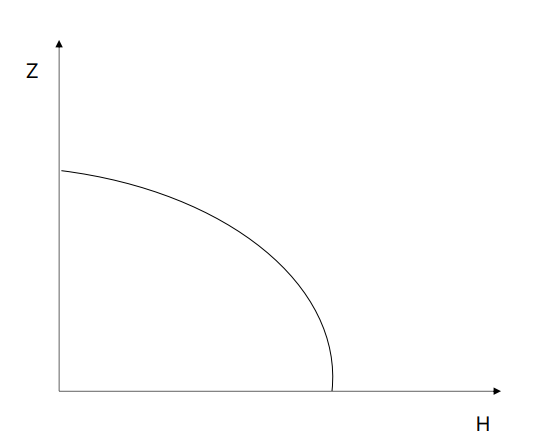
\includegraphics[width=3in]{images/ch3/23.png}
                \caption{Wrong PPF}
                \label{fig:label}
            \end{figure}

When H=0, we can't do anything, so we need to have $H_{min}$. 

\item Correct PPF:

\begin{figure}[H]%option [H] means "strictly here"
                \centering
                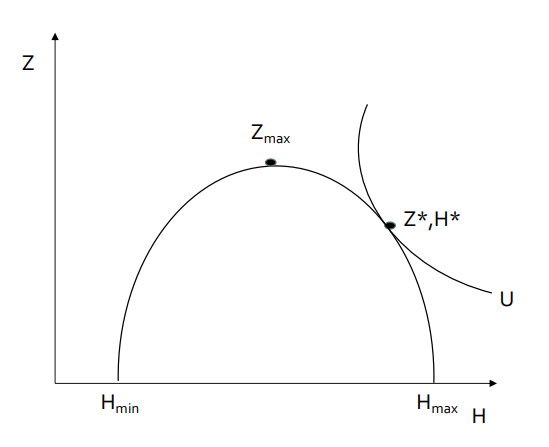
\includegraphics[width=3in]{images/ch3/24.png}
                \caption{Correct PPF}
                \label{fig:label}
            \end{figure}

We must have $H_{min}$, $Z_{max}$, and $H_{max}$.  We reach the optimal point when the indifference curve is tangent to the PPF.
\end{itemize} 

\subsection{The Demand for Health}
\begin{itemize}
        \item \textcolor{red}{Optimality conditions (simplest version of the model):}

        \textcolor{red}{PV of the marginal cost of gross investment = PV of marginal benefits of health}
        
        \textcolor{red}{(MEC curve intersects with COC curve)}

        \item The marginal returns of health capital are represented by the \textcolor{red}{Marginal Efficiency of Health Capital (MEC) curve}. i.e. the value of the additional healthy days gained from a 1-unit increase in the health stock (MPH). MEC is the monetary value of the marginal productivity of health stocks. It is declining.
        
        \textcolor{red}{MEC=MPH*w}
       
        w: wage rate
        
        MPH: marginal productivity of health stock

        \item The \textcolor{red}{Cost of Capital (COC) curve} represents the supply price of capital or the cost of holding an additional unit. Its position is determined by the depreciation rate of the health stock ($\delta$) and the opportunity cost of holding health capital (r).

\begin{figure}[H]%option [H] means "strictly here"
                \centering
                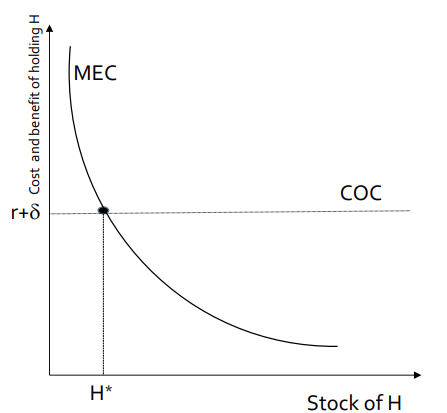
\includegraphics[width=3in]{images/ch3/25.png}
                \caption{MEC and COC of holding health stocks}
                \label{fig:label}
            \end{figure}
\end{itemize} 

\subsubsection{What happens as we age?}
\begin{figure}[H]%option [H] means "strictly here"
                \centering
                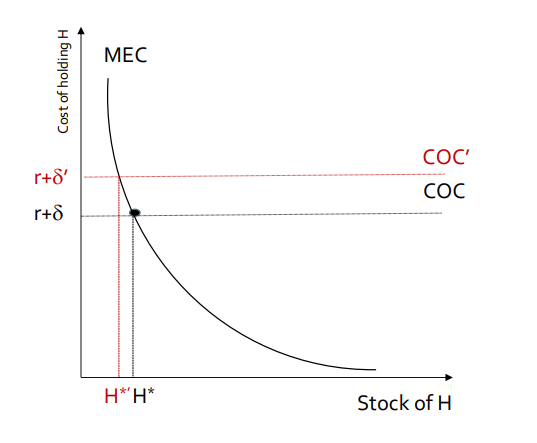
\includegraphics[width=3in]{images/ch3/26.png}
                \caption{What happens as we age?}
                \label{fig:label}
            \end{figure}

\begin{itemize}
        \item The depreciation rate ($\delta$) increases when ageing, so the COC shifts upwards to COC', and the optimal level of health stock we can sustain is lower (H*').
\end{itemize} 

\subsection{How the Literature has Developed}
\begin{itemize}
        \item Since 1972, the Grossman model has been the cornerstone for modelling
investment in health capital, spurring a great deal of research, extensions, 
empirical testing and criticism.
        \item Grossman himself reviewed the literature many times, e.g. in the 2000 Chapter “The Human Capital Model” in the Handbook of Health Economics.
        \item Some of the main criticisms of the Grossman model:
        \begin{enumerate}
            \item It does not preclude an individual choosing to live forever (Ehrlich and Chuma, JPE 1990 “does not determine the length of life")
            \item It does not provide an adequate conceptual framework for the SES (socioeconomic status)-health: They develop a model which incorporates health, longevity, wealth, earnings, education, work, job-related physical and psychosocial health stressors, leisure, health investment (e.g. exercise, medical care) and healthy and unhealthy consumption (including housing, neighbourhood social environment).
            \item Not faithful to gerontological models of health deficit accumulation (Strulik).
            \item It does not include an early childhood phase (Heckman, PNAS 2007).
gradient (Galama and van Kippersluis, EJ, 2018).
        \end{enumerate}
        \item Very active area of research, both theoretically and empirically.
\end{itemize}

\section{Inequalities in Health}
Inequalities in health are not random and are associated with characteristics. Poor people are less healthy, maybe because they eat cheaper food, don't know the benefit of doing exercise (less educated). Education is correlated with health. 
More educated  $\Rightarrow$  Higher income  $\Rightarrow$  More resources and information

\subsection{SES Inequalities in BMI Widen over the Lifecycle and across British Cohorts}
\begin{figure}[H]%option [H] means "strictly here"
                \centering
                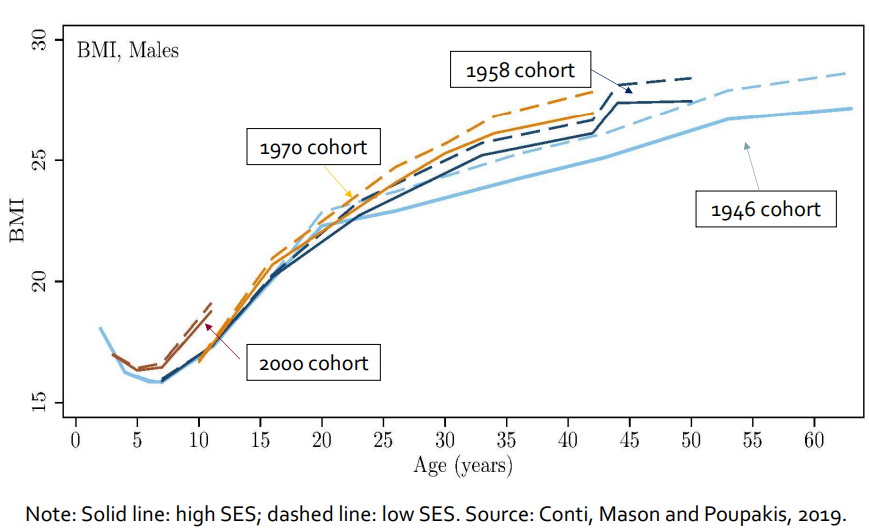
\includegraphics[width=4in]{images/ch3/27.png}
                \caption{SES Inequalities in BMI Widen over the Lifecycle and across British Cohorts}
                \label{fig:label}
            \end{figure}
\begin{itemize}
        \item BMI (Body Mass Index) is not the best measure of body fitness, since it only includes two dimensions (weight and height), it doesn't take into account fat mass, it doesn't include many diseases such as blindness, it is developed in the West and thus the norms may not apply to other ethnicities. However, BMI is a relatively simple measure, and it is correlated with obesity and worse body conditions later in life.
        \subsubsection{Lifecycle:}
        \item The lines are very close in the beginning, the 1946 cohort starts to diverge at the end of adolescence and keeps diverging as they get older. 
        \item Low SES people have higher BMIs than high SES people as they get older.
        \item For each cohort, BMI generally increases as age increases. 
        \subsubsection{Cohort:}
        \item 2000 cohort has a higher BMI at the young age.
        \item The health inequality (divergence) is present in every cohort, and we are not doing anything to effectively reduce it.
\end{itemize}       
        
\subsection{Health inequalities are everywhere}
\begin{itemize}
        \item Researchers have documented inequalities in the distribution of health by socioeconomic status, gender, and ethnicity.
        \item Research on socio-economic inequalities in health in the UK has a long history
        \item In the early part of the 20th century the British government introduced questions on occupation in the decennial census.
        \item The 1970-1972 Decennial Supplement of occupational Mortality (OCPS) showed that men in social class V (unskilled) were 2.5 times as likely to die before the age of 65 than those in social class I (professional). Children in social class V families were twice as likely to die as those in social class I.
\end{itemize} 

\subsection{Landmark studies in social class inequalities in health in the UK include:}
\begin{itemize}
        \item Black Report (1980)
        \begin{enumerate}
            \item Health inequalities were widening, the problem had little to do with NHS.
            \item Four possible explanations: (1) data artefact; (2) social selection (sicker people $\Rightarrow$ less able to study and work $\Rightarrow$ poorer); (3) behaviour; (4) material circumstances.
            \item Policy recommendation: reduce poverty, spend more on prevention.
        \end{enumerate}
        
        \item Whitehead Report (1987)
        \begin{enumerate}
            \item Commissioned by the Health Education Council (HEC) and headed by
Margaret Whitehead.
            \item Health inequalities widened since the Black Report.
            \item HEC was scrapped: was campaigning on alcohol, tobacco and diet issues which upset some of the government’s financial supporters.
        \end{enumerate}
        
        \item Acheson Report (1998)
        \begin{enumerate}
            \item Commissioned by the new Labour (Blair) government in 1997, under the chairmanship of a former Chief Medical Officer, Sir Donald Acheson.
            \item Similar findings and recommendations as the Black Report: the root cause of inequalities in health was poverty.
        \end{enumerate}

        \item Whitehall I Study
        \begin{enumerate}
            \item Examined over 18,000 male British civil servants over 10 years, starting in 1967.
            \item Showed that mortality was higher among those in the lower grade than in the higher grade – for all causes and CHD.
            \item Controlling for risk factors (smoking, obesity, exercise, blood pressure) accounted for 40 percent of the gradient.
        \end{enumerate}

        \item Whitehall II Study
        \begin{enumerate}
            \item Examined 10,308 civil servants aged 35-55, 2/3 men and 1/3 women, starting in 1985.
            \item Showed social gradient for several diseases.
            \item Added job-related stress to the traditional risk factors for low social class.
        \end{enumerate}

        \item Fair Society, Healthy Lives: The Marmot Report (2010)
        \begin{enumerate}
            \item Concluded that reducing health inequalities would require action on six policy objectives: number 1 is “Give every child the best start in life”.
        \end{enumerate}

        \item Health Equity in England: The Marmot Review 10 Years On (2020)
        \begin{enumerate}
            \item “This ‘10 years on’ report shows that, in England, health is getting worse for people living in more deprived districts and regions, health inequalities are increasing  and, for the population as a whole, health is declining. The data that this report brings together also show that for almost of all the recommendations made in the original Marmot Review, the country has been moving in the wrong direction. In particular, lives for people towards the bottom of the social hierarchy have been made more difficult. Some of these difficulties have been the direct result of government policies, some have resulted from failure to counter adverse trends such as increased economic inequalities or market failures.”
        \end{enumerate}
\end{itemize} 

\subsubsection{The Marmot Review}
\begin{figure}[H]%option [H] means "strictly here"
                \centering
                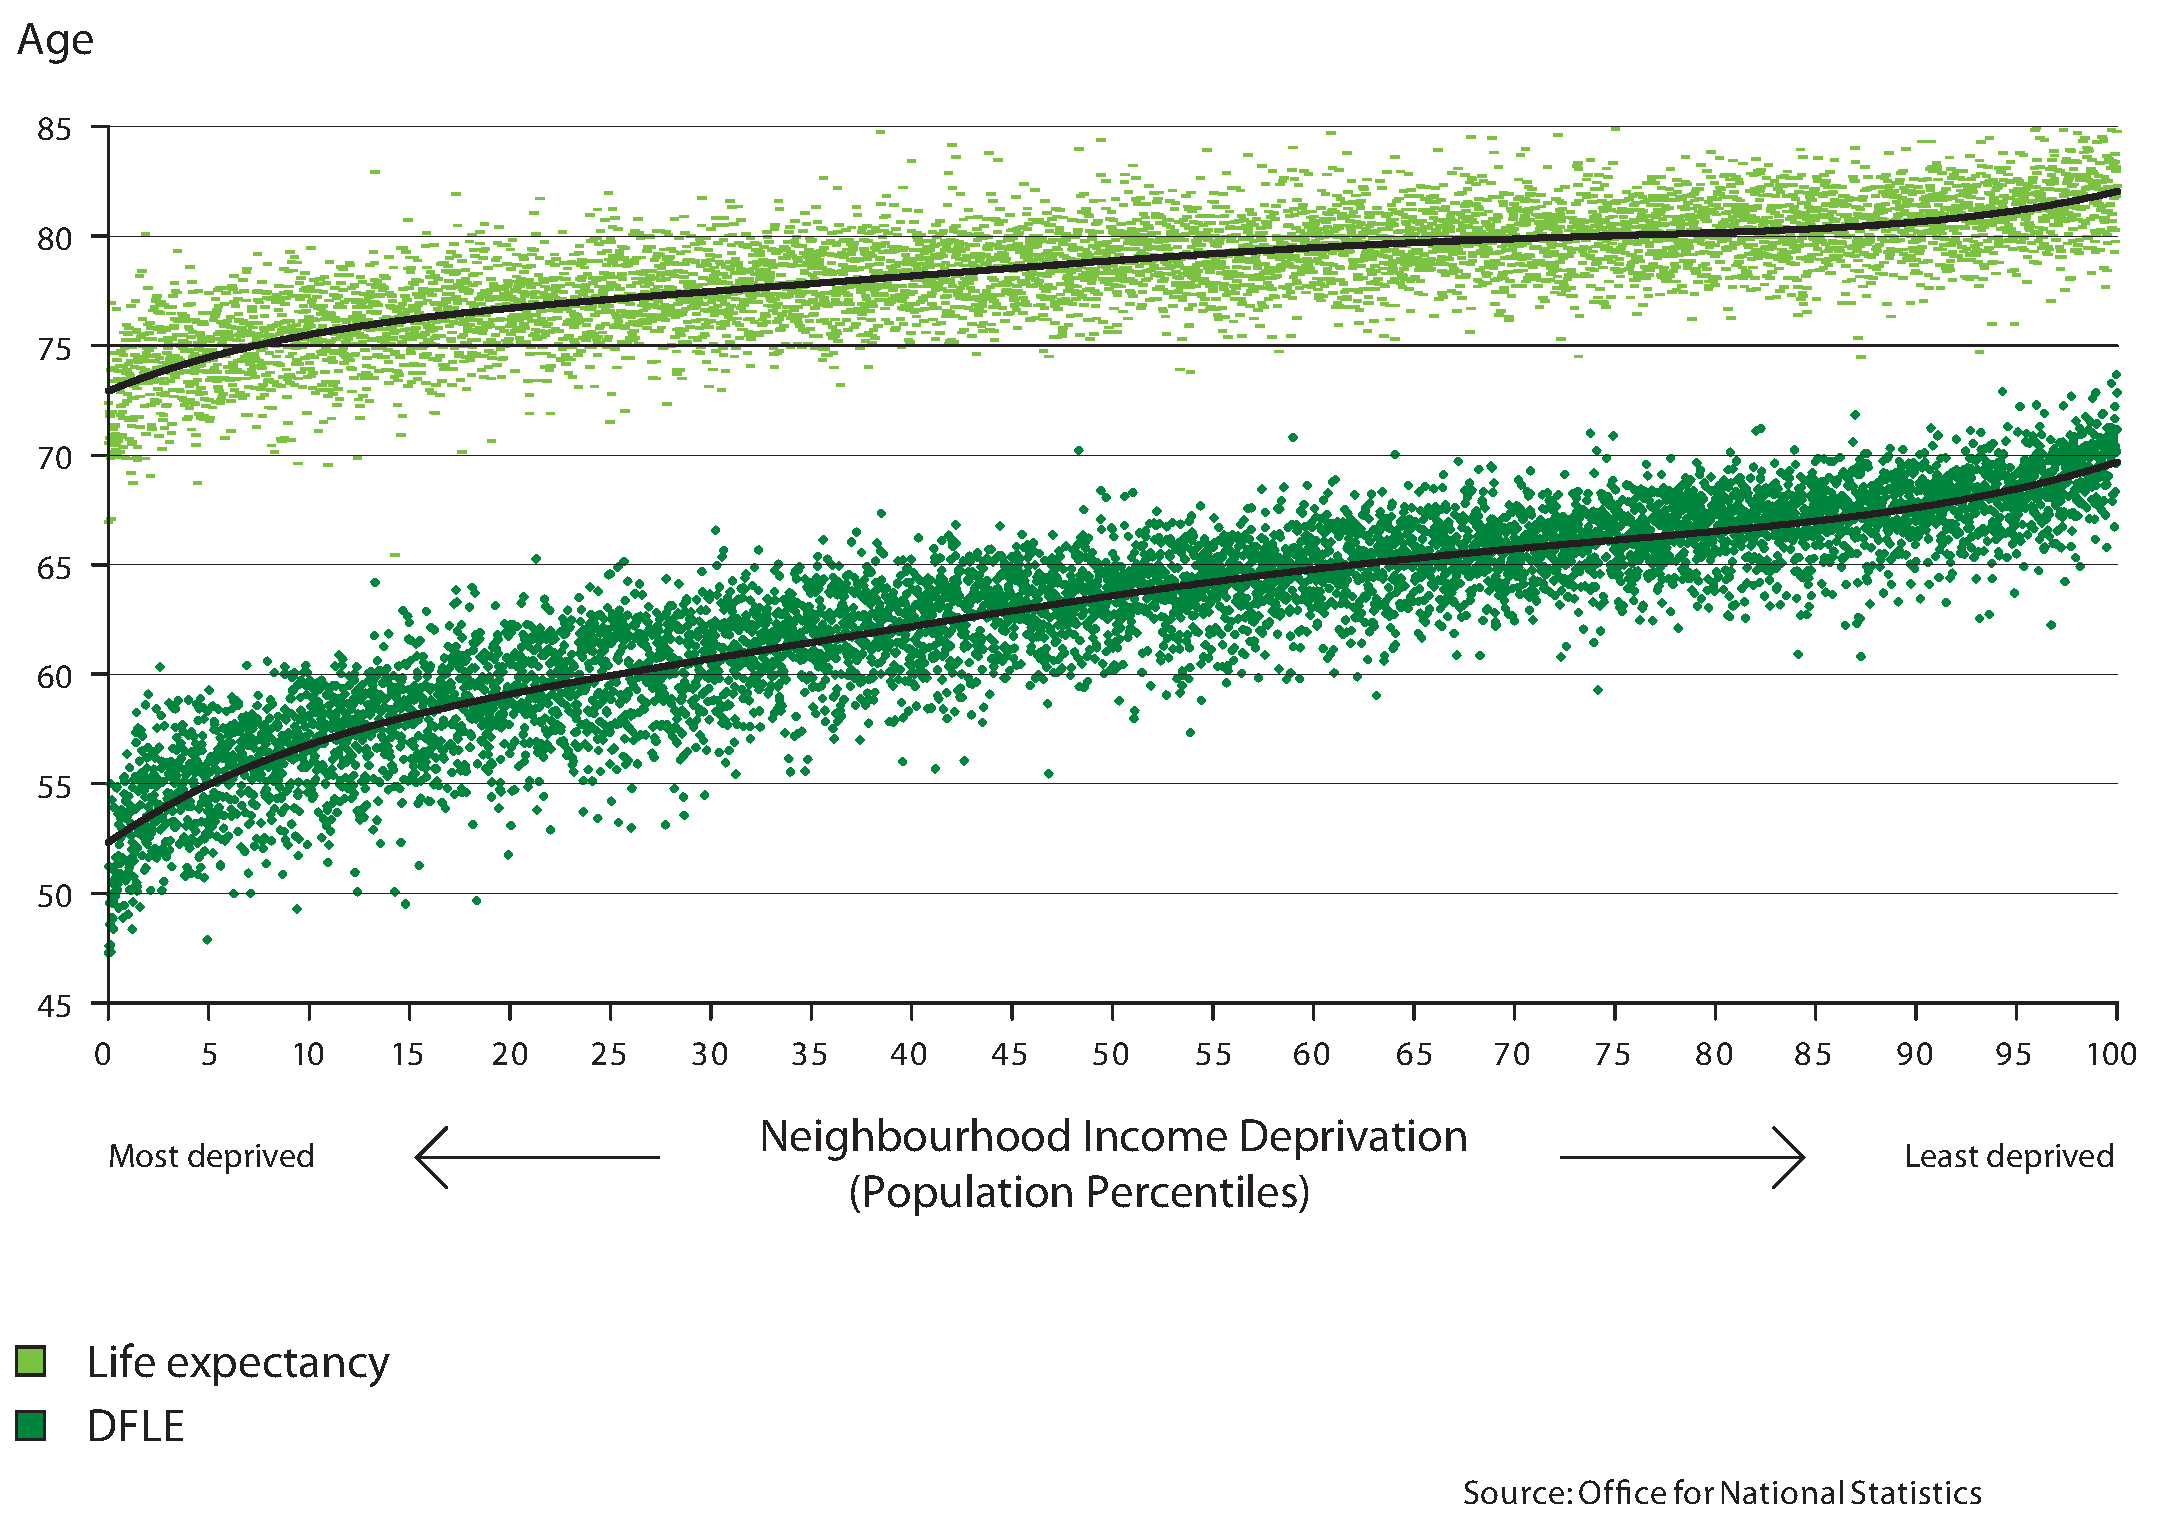
\includegraphics[width=4in]{images/ch3/28.png}
                \caption{Life expectancy and disability-free life expectancy (DFLE) at birth, by neighbourhood income level, England, 1999-2003}
                \label{fig:label}
            \end{figure}
\begin{itemize}
        \item DFLE measures not only how long you live but also how well you live, so there is a gap between life expectancy and DFLE.
        \item There is a discrepancy in the life expectancy/DFLE between the most deprived and the least deprived people in England.
\end{itemize} 

\begin{figure}[H]%option [H] means "strictly here"
                \centering
                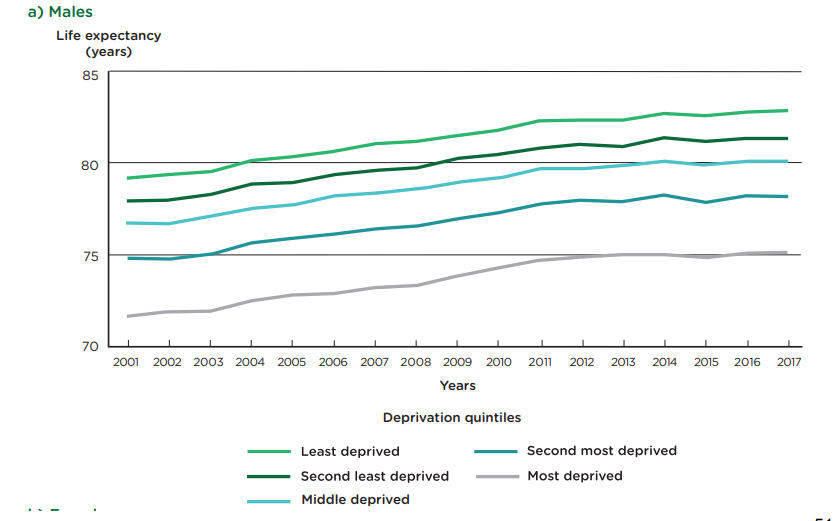
\includegraphics[width=4in]{images/ch3/29.png}
                \caption{Life expectancy at birth by area deprivation quintiles and sex, England, 2003–05 to 2015–17}
                \label{fig:label}
            \end{figure}
\begin{itemize}
        \item Life expectancy is increased for everyone.
        \item The most deprived has the lowest life expectancy.
        \item The gaps between groups are almost the same as time passed, so inequalities stay the same.
\end{itemize}

\subsubsection{Public Health England}
\begin{figure}[H]%option [H] means "strictly here"
                \centering
                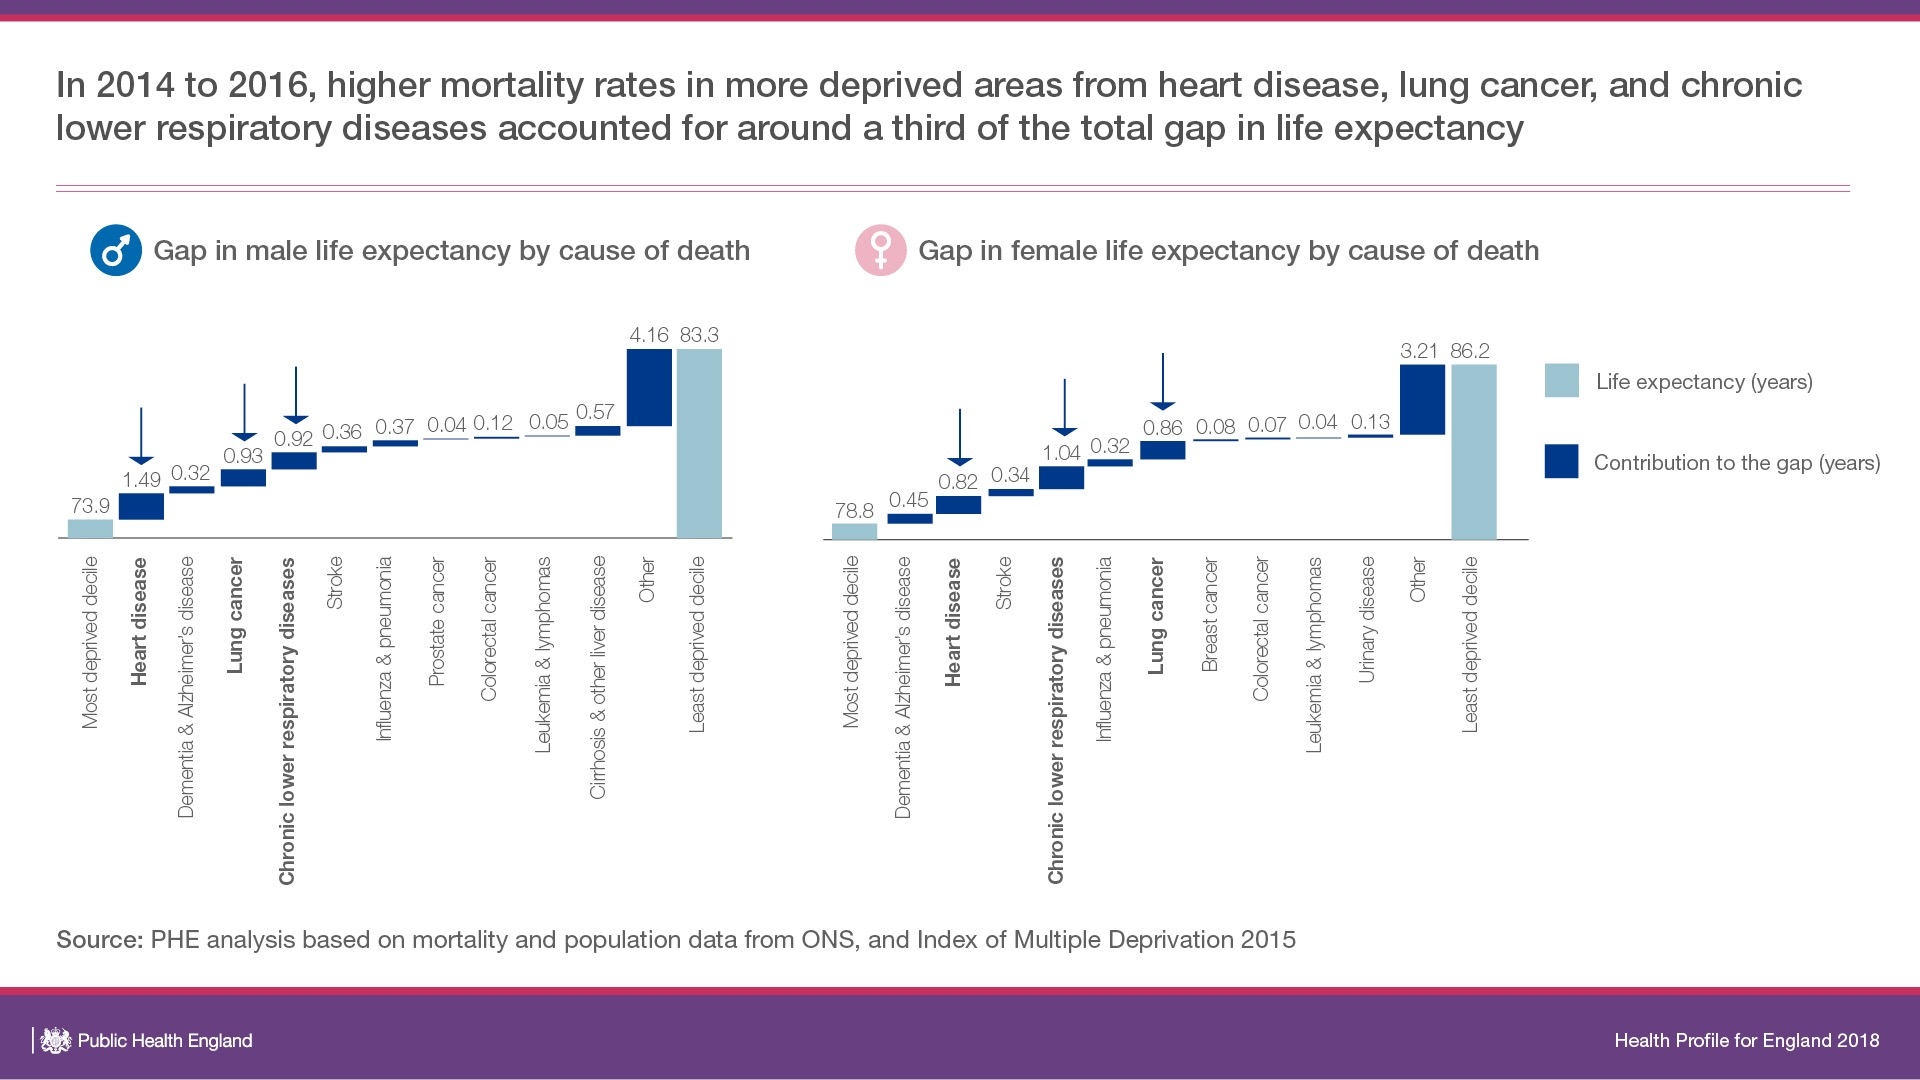
\includegraphics[width=5in]{images/ch3/30.png}
                \caption{What causes of death are driving the gap in life expectancy among the most deprived people and the least deprived people, male/female}
                \label{fig:label}
            \end{figure}
\begin{itemize}
        \item In 2014 to 2016, higher mortality rates in more deprived areas from heart disease, lung cancer, and chronic lower respiratory diseases accounted for around a third of the total gap in life expectancy.
\end{itemize}

\subsubsection{The IFS Deaton Review (2019-)}

\begin{figure}[H]%option [H] means "strictly here"
                \centering
                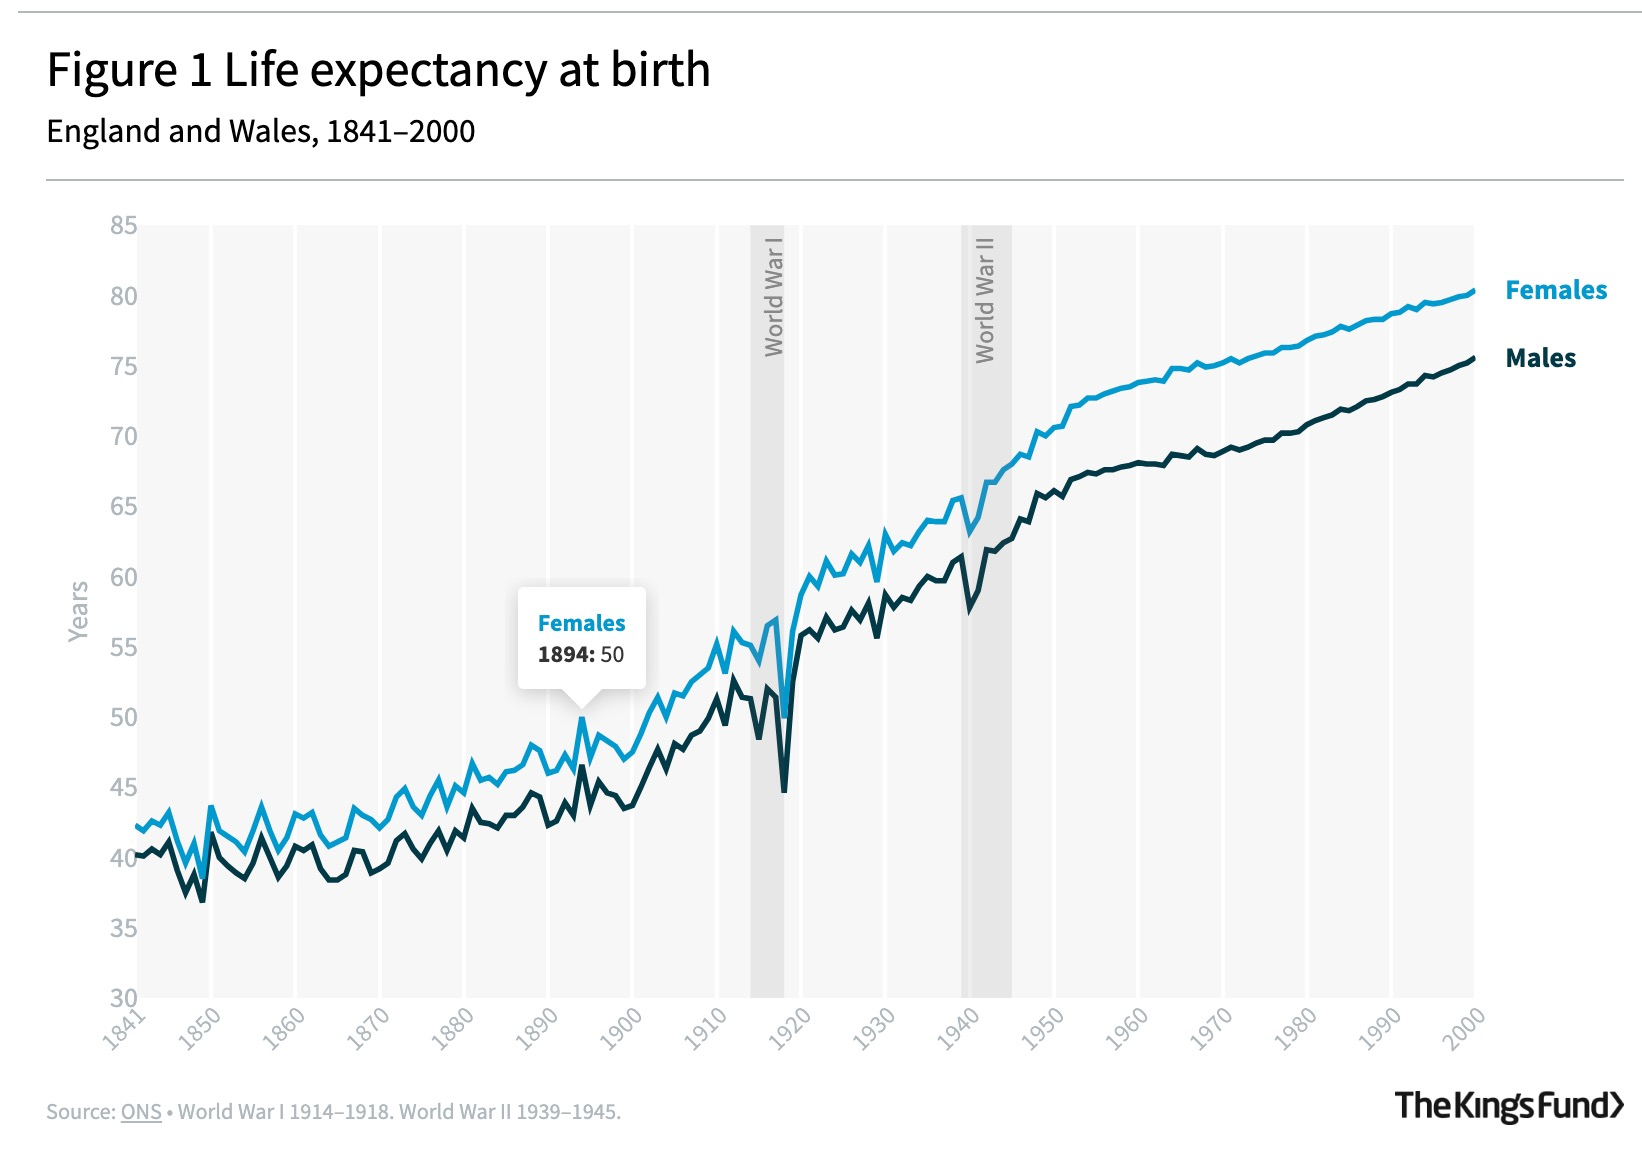
\includegraphics[width=4in]{images/ch3/31.png}
                \caption{Life expectancy at birth, England and Wales, 1841-2000, Males/Females}
                \label{fig:label}
            \end{figure}
\begin{itemize}
        \item The life expectancy increased and almost doubled. Females had higher life expectancy. The biggest drop was in World War II.
\end{itemize}
 
\begin{figure}[H]%option [H] means "strictly here"
                \centering
                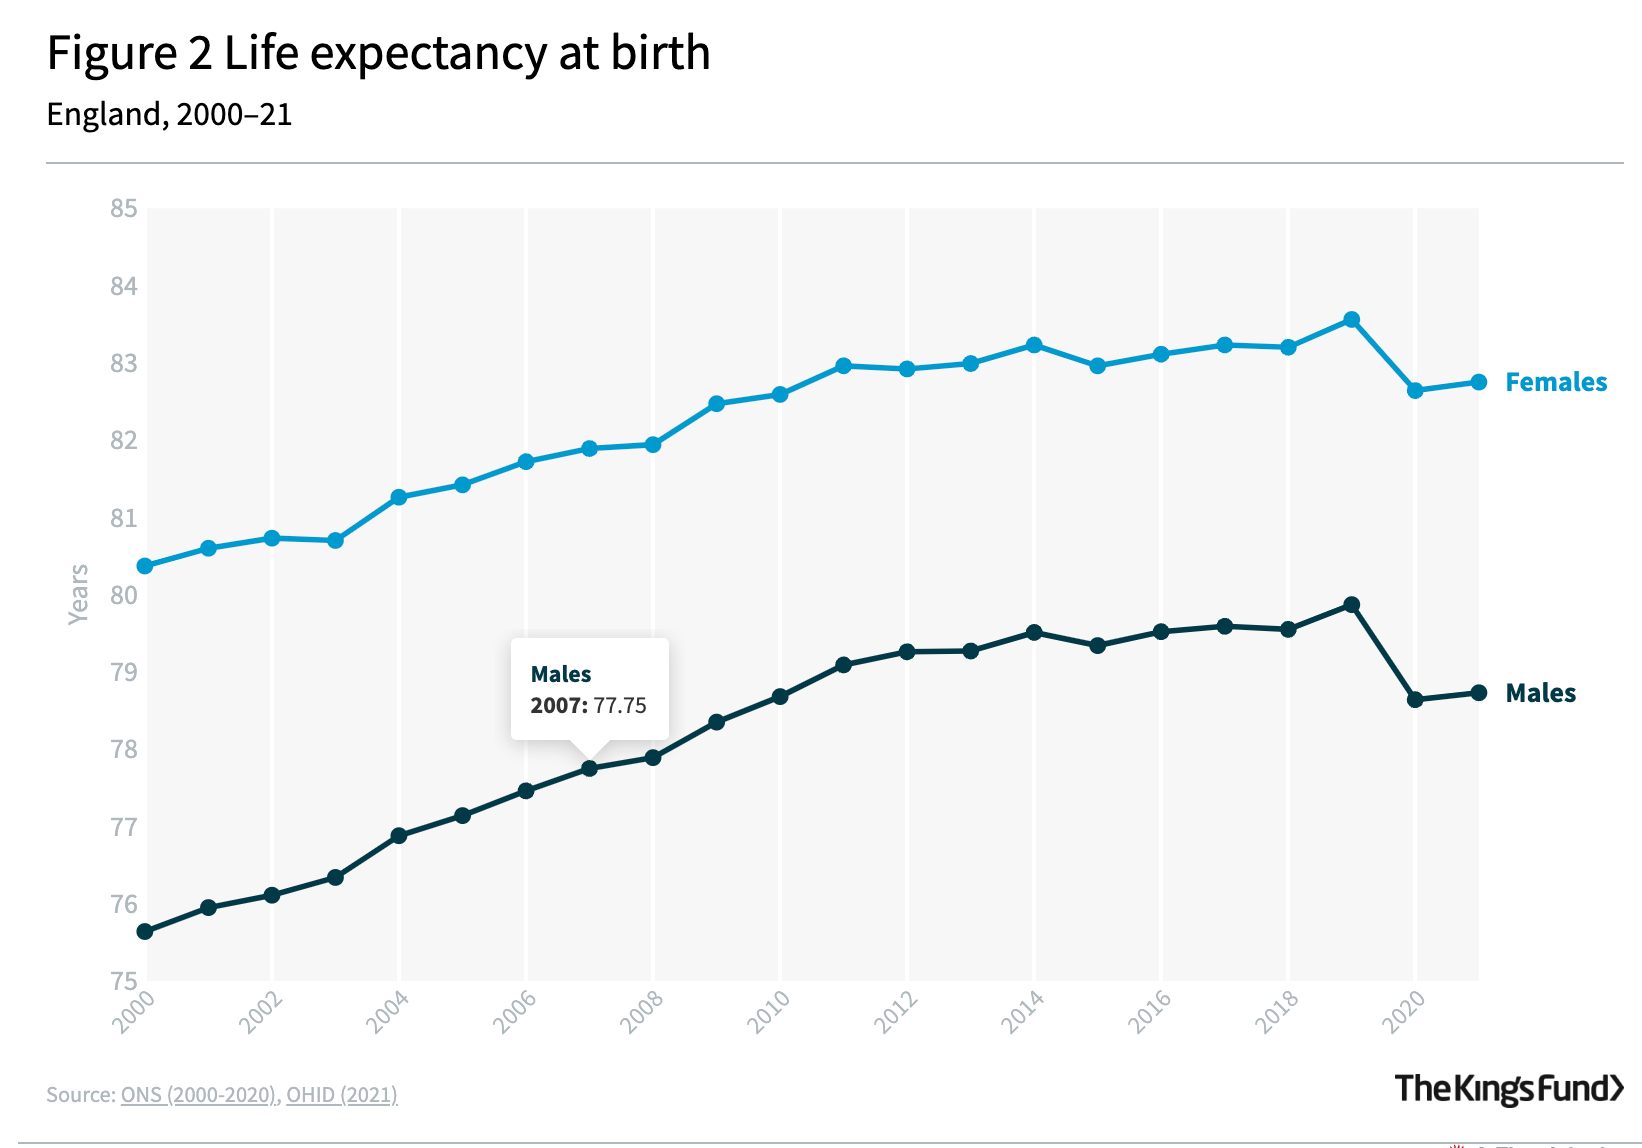
\includegraphics[width=4in]{images/ch3/32.png}
                \caption{Life expectancy at birth, England, 2000-2021, Males/Females}
                \label{fig:label}
            \end{figure}        
\begin{itemize}
        \item The second biggest drop was during the pandemic (about 1 year).
\end{itemize}     

\begin{figure}[H]%option [H] means "strictly here"
                \centering
                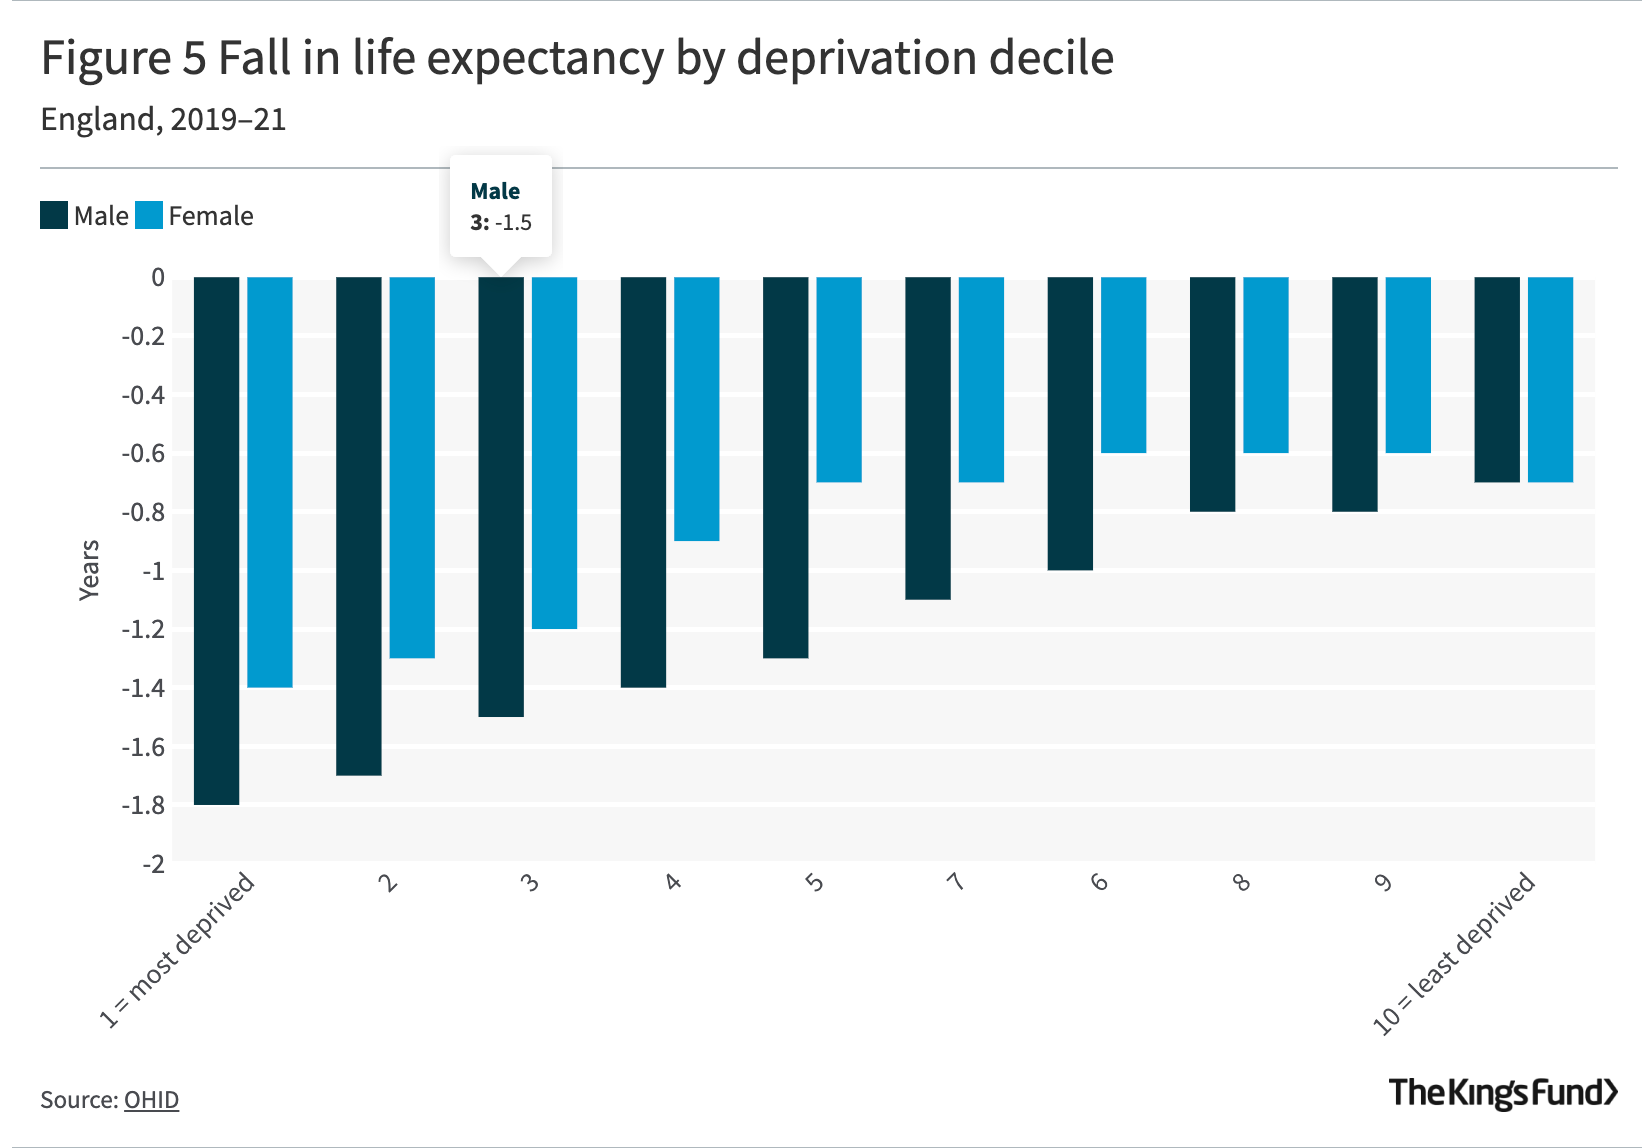
\includegraphics[width=4in]{images/ch3/33.png}
                \caption{Fall in life expectancy by deprivation decile, England, 2019-21}
                \label{fig:label}
            \end{figure}        
\begin{itemize}
        \item During the Covid-19 pandemic, the most deprived male had a life expectancy drop of 1.8 years, while the least deprived male had a life expectancy drop of 0.7 years. Males tend to have a bigger drop than females. 
\end{itemize}   

\subsection{Why Do Health Disparities Exist?}
\begin{itemize}
        \item SES can causally affect health. In terms of the Grossman model:
        \begin{enumerate}
            \item Different SES groups can have different MECs (e.g. high vs. low education).

            \textcolor{red}{MEC=MPH*w} 

            higher wage, higher MEC

            
            \item High SES individuals can have an expanded PPF because of extra financial resources.
            \item Low SES individuals can have a higher $\delta$ because of stress.
        \end{enumerate}
        \item Early health can causally affect SES (health selection).

        e.g. unhealthy child $\Rightarrow$ less educated $\Rightarrow$ lower SES
        
        \item Both can be affected by third factors.
        
        e.g. time preferences (Fuchs’ hypothesis): people willing to delay gratification (high $\delta$) invest more in both health and education.

        \item Understanding the causes of health disparities is of key policy importance for addressing them (health subsidies, health information, nudge, for the poor people).
\end{itemize}

\section{Education and Health}
\subsection{Disparities by Education (compulsory vs. post-compulsory)}
\begin{figure}[H]%option [H] means "strictly here"
                \centering
                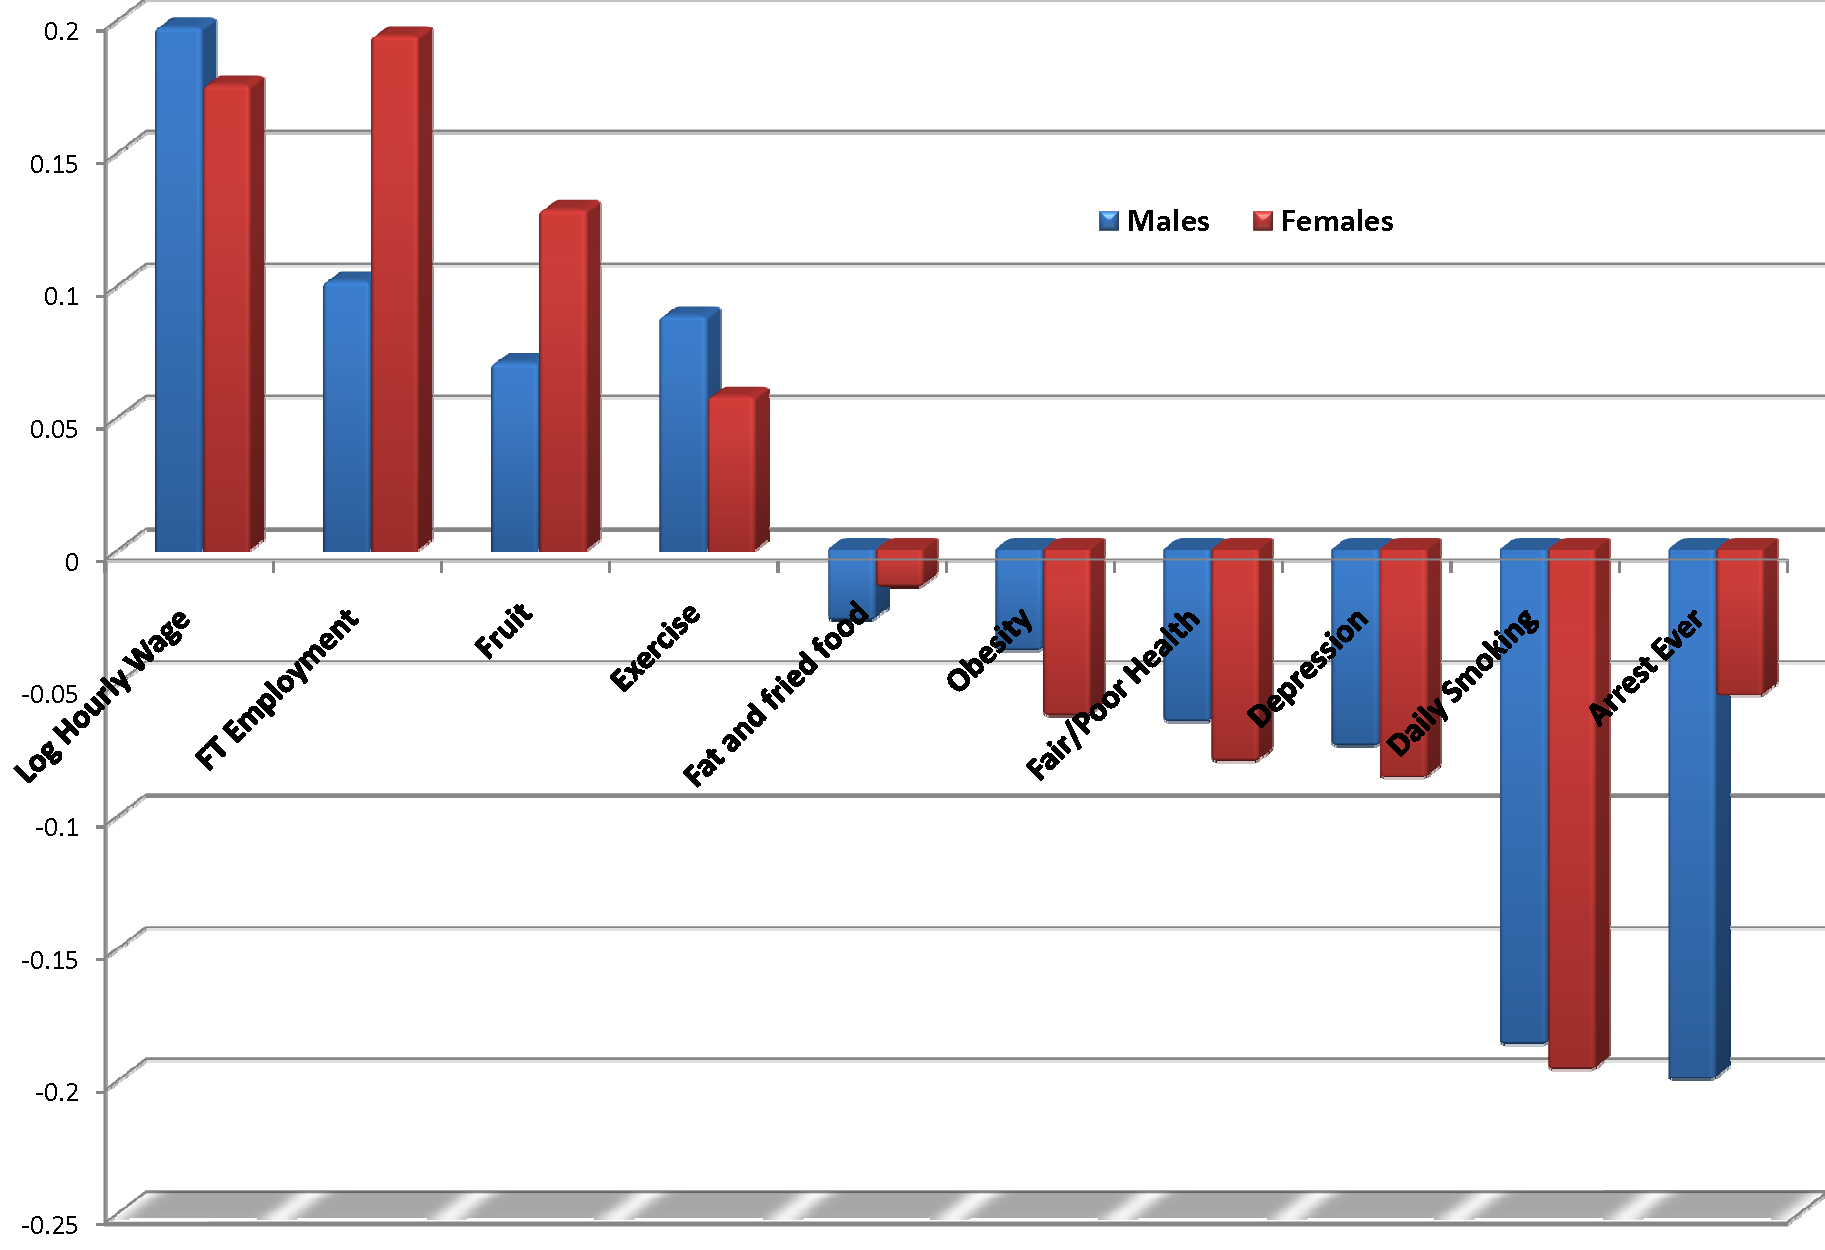
\includegraphics[width=4in]{images/ch3/34.png}
                \caption{Disparities by Education (compulsory vs. post-compulsory)}
                \label{fig:label}
            \end{figure}    
\begin{itemize}
        \item The graph shows the raw differentials in the outcomes between individuals with post-compulsory and compulsory level of education.          Individuals with post-compulsory education tend to have better health.
\end{itemize}

\subsection{Causality or Correlation?}
\begin{itemize}
        \item \textcolor{red}{Is the positive correlation between health and schooling causal?}
        \item Literature has used different approaches to establish causality.
        \begin{enumerate}
            \item First set of studies: used instrumental variables with questionable instruments for education (e.g. quarter of birth), finding strong effects.
            \item Second set of studies: exploited features of the educational system.
            
            (a) Lleras-Muney (RevStud, 2005) uses compulsory school and child labour laws in thirty states from 1915 to 1939 as instruments for education and finds a significant effect in reducing mortality (using DiD).

            (b) Clark and Royer (AER, 2013) use regression discontinuity methods (RDD) exploiting two changes to British compulsory schooling laws and find no effects on mortality or other measures of health. Similar results in a recent paper by Janke, Johnston, Propper et al. (JHE, 2018).

             \item Third set of studies: twin differences (Lundborg, JPopEc 2013).
             \item Fourth set of studies: more “structural” models (Conti et al., 2010a,b; Heckman et al., 2018).
        \end{enumerate}
\end{itemize} 

\subsubsection{Twin differences (Lundborg, JPopEc 2013)}
\begin{itemize}
        \item $$Y_i = \alpha_0+\alpha_1 eduyrs_i+\alpha_2 X_i+\eta_i$$
        where  $Y_i$ is the BMI of one twin

Take the difference between twins' BMIs:

$$\Delta Y = \beta_0+\beta_1\Delta eduyrs+\beta_2 \Delta X+\Delta \eta$$
where  $\Delta Y=Y_i-Y_j$ 

This is a fixed-effect regression.

$\beta_1$ will not be interpreted as the causal effect of education on health, as education is a choice, which is likely to be correlated with the error term (ability/effort/parents' investment), so we need an instrument for $\Delta eduyrs$.

\item However, if we estimate

$$\Delta Y = \gamma_0+\gamma_1\Delta BW+\gamma_2 \Delta X+\Delta \eta$$

where BW is the birth weight,

$\gamma_1$ may estimate the causal effect of birth weight difference on BMI difference, as birth weight is predetermined.
\end{itemize} 

\subsubsection{Clark and Royer RDD (AER, 2013)}
\begin{figure}[H]%option [H] means "strictly here"
                \centering
                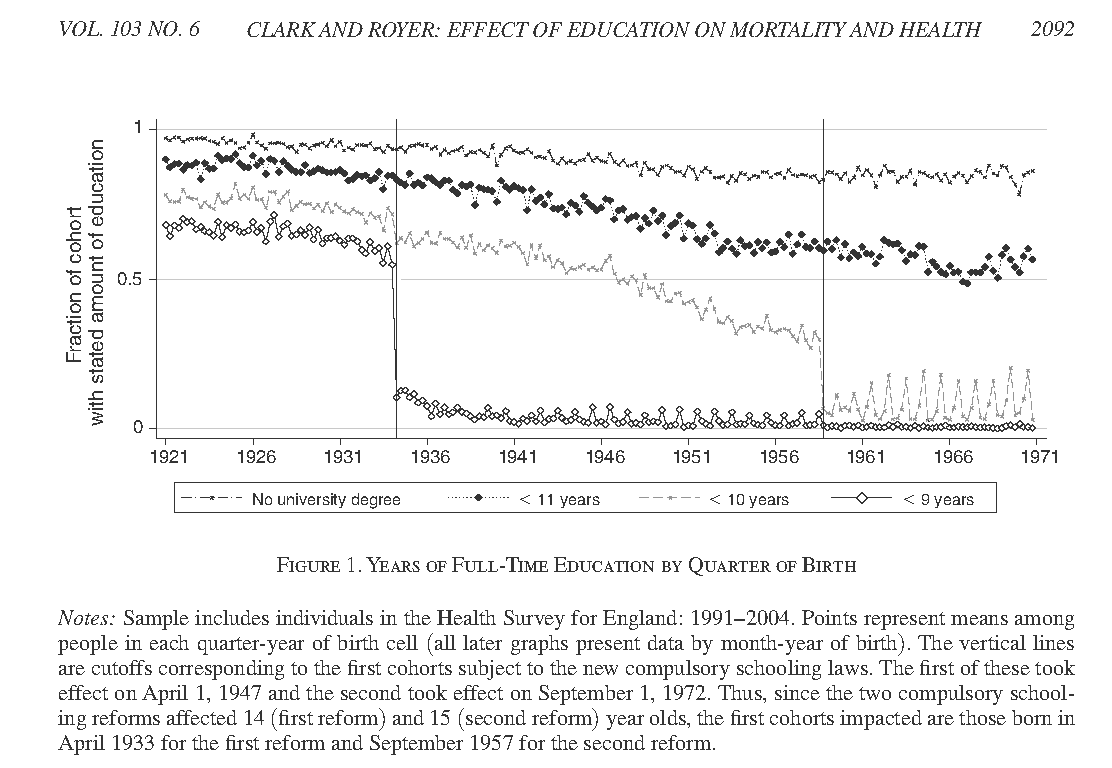
\includegraphics[width=4in]{images/ch3/35.png}
                \caption{Years of Full-Time Education by Quarter of Birth}
                \label{fig:label}
            \end{figure}
            
\begin{itemize}
        \item This figure presents data at the quarter-of-birth level using Health Survey of England data. We study how the introduction of two compulsory schooling laws affected the fraction of cohorts with stated amount of education. The first reform took effect on April 1, 1947, which increased the compulsory school leaving age from 14 to 15, and the second took effect on September 1, 1972, which increased the compulsory school leaving age from 15 to 16. The vertical lines are cutoffs corresponding to the first cohorts subject to the new compulsory schooling laws. Since the two compulsory schooling reforms affected 14 (first reform) and 15 (second reform) years old, the first cohorts impacted are those born in April 1933 for the first reform and September 1957 for the second reform.
                 
        \item The 1947 change reduced the fraction that completed nine years or less by roughly one half; the 1972 change decreased the fraction that completed ten years or less by roughly one quarter. Hence, the reforms did increase students' years of education and reduce the number of students who dropped out at a particular age.
\end{itemize}
       
\begin{figure}[H]%option [H] means "strictly here"
                \centering
                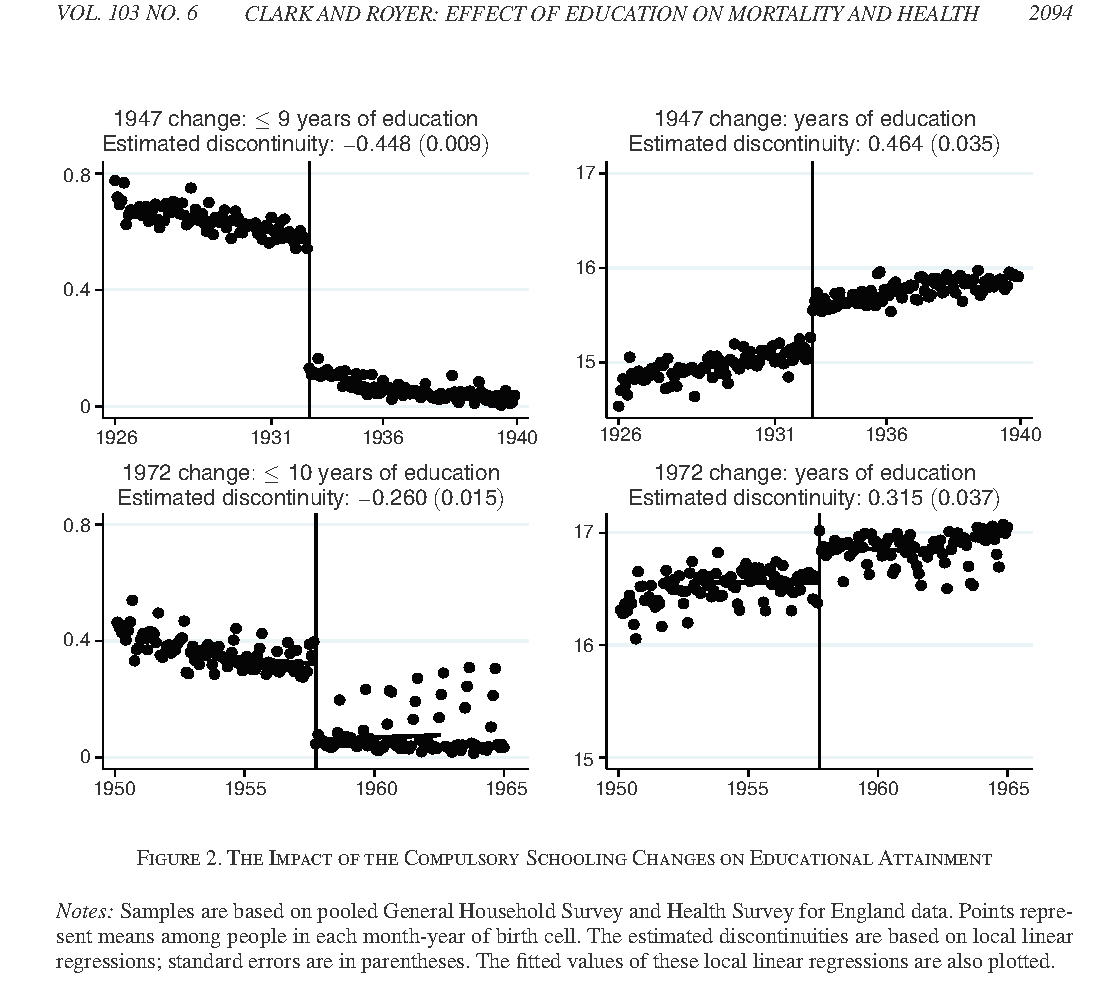
\includegraphics[width=3in]{images/ch3/36.png}
                \caption{The Impact of the Compulsory Schooling Changes on Educational Attainment}
                \label{fig:label}
            \end{figure}

\begin{itemize}
        \item To examine the effect of the law changes on educational attainment, we begin by graphing the relationship between the birth cohort and the probability of completing less than nine and less than ten years of education.
        \item The 1947 change reduced the fraction of individuals completing nine or fewer years of education by around 0.5. The 1972 change decreased the fraction completing ten or fewer years of education by around 0.25.
        \item The 1947 change increased the years of education of the 1933 cohort by around 0.5 years. The 1972 change increased the years of education of the 1957 cohort by around 0.3 years.
\end{itemize}


\begin{figure}[H]%option [H] means "strictly here"
                \centering
                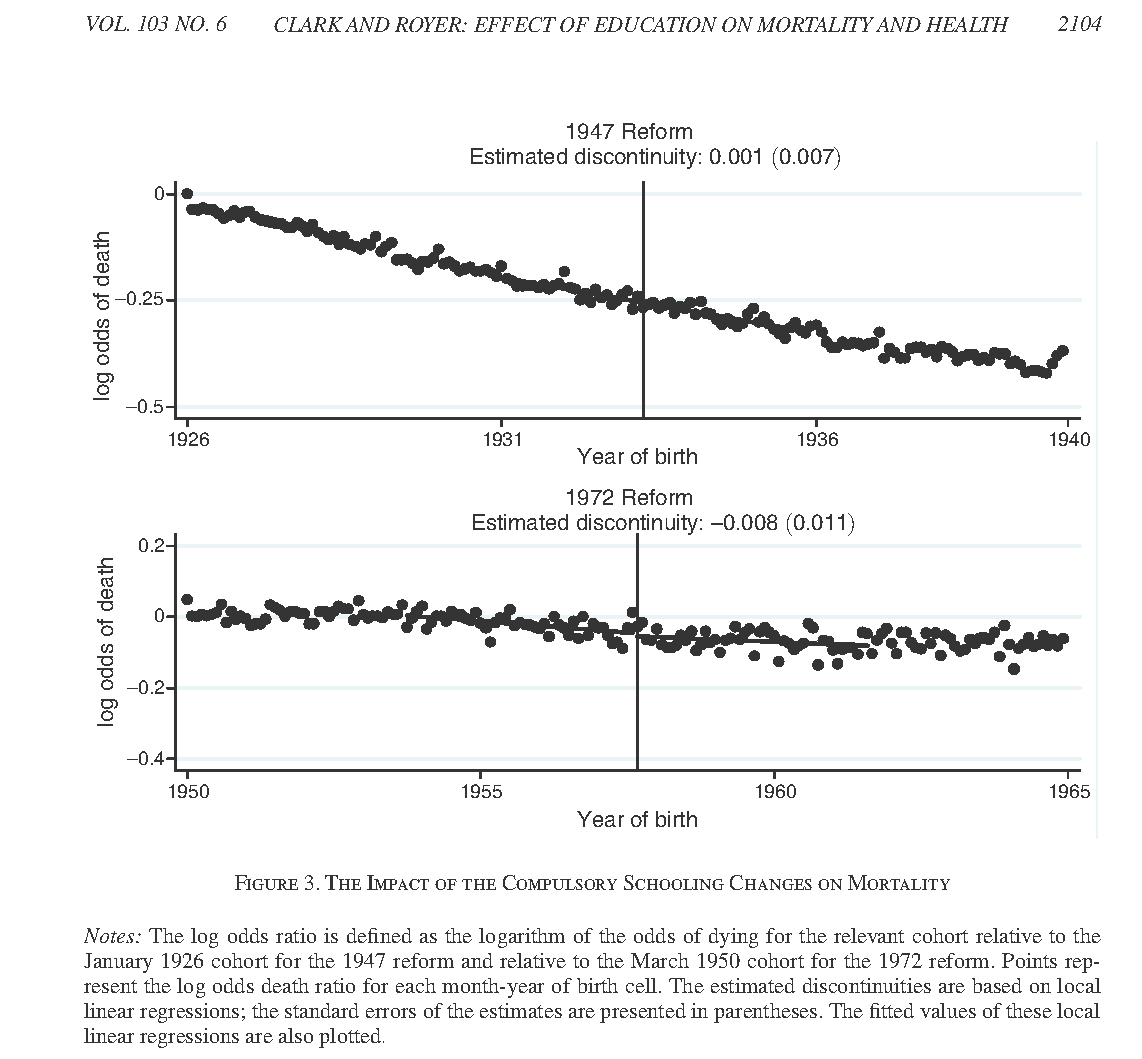
\includegraphics[width=3in]{images/ch3/37.png}
                \caption{The Impact of the Compulsory Schooling Changes on Mortality}
                \label{fig:label}
            \end{figure}

\begin{itemize}
        \item The two compulsory schooling laws have no effect on mortality (no discontinuity).
\end{itemize}        

\begin{figure}[H]%option [H] means "strictly here"
                \centering
                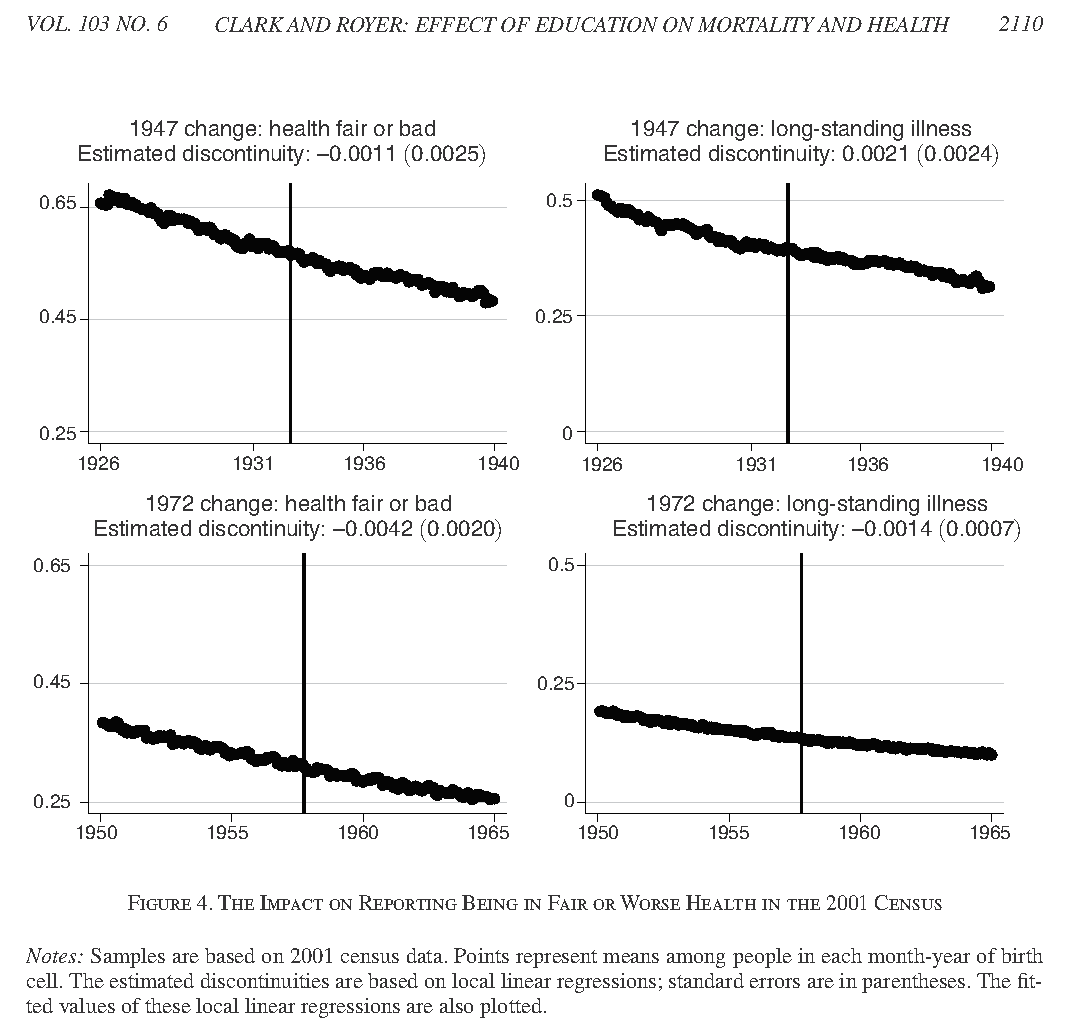
\includegraphics[width=3in]{images/ch3/38.png}
                \caption{The Impact on Reporting Being in Fair or Worse Health in the 2001 Census}
                \label{fig:label}
            \end{figure}  

\begin{itemize}
        \item The reforms cause no change in health fair or bad and long-standing illness.

\end{itemize}

\begin{figure}[H]%option [H] means "strictly here"
                \centering
                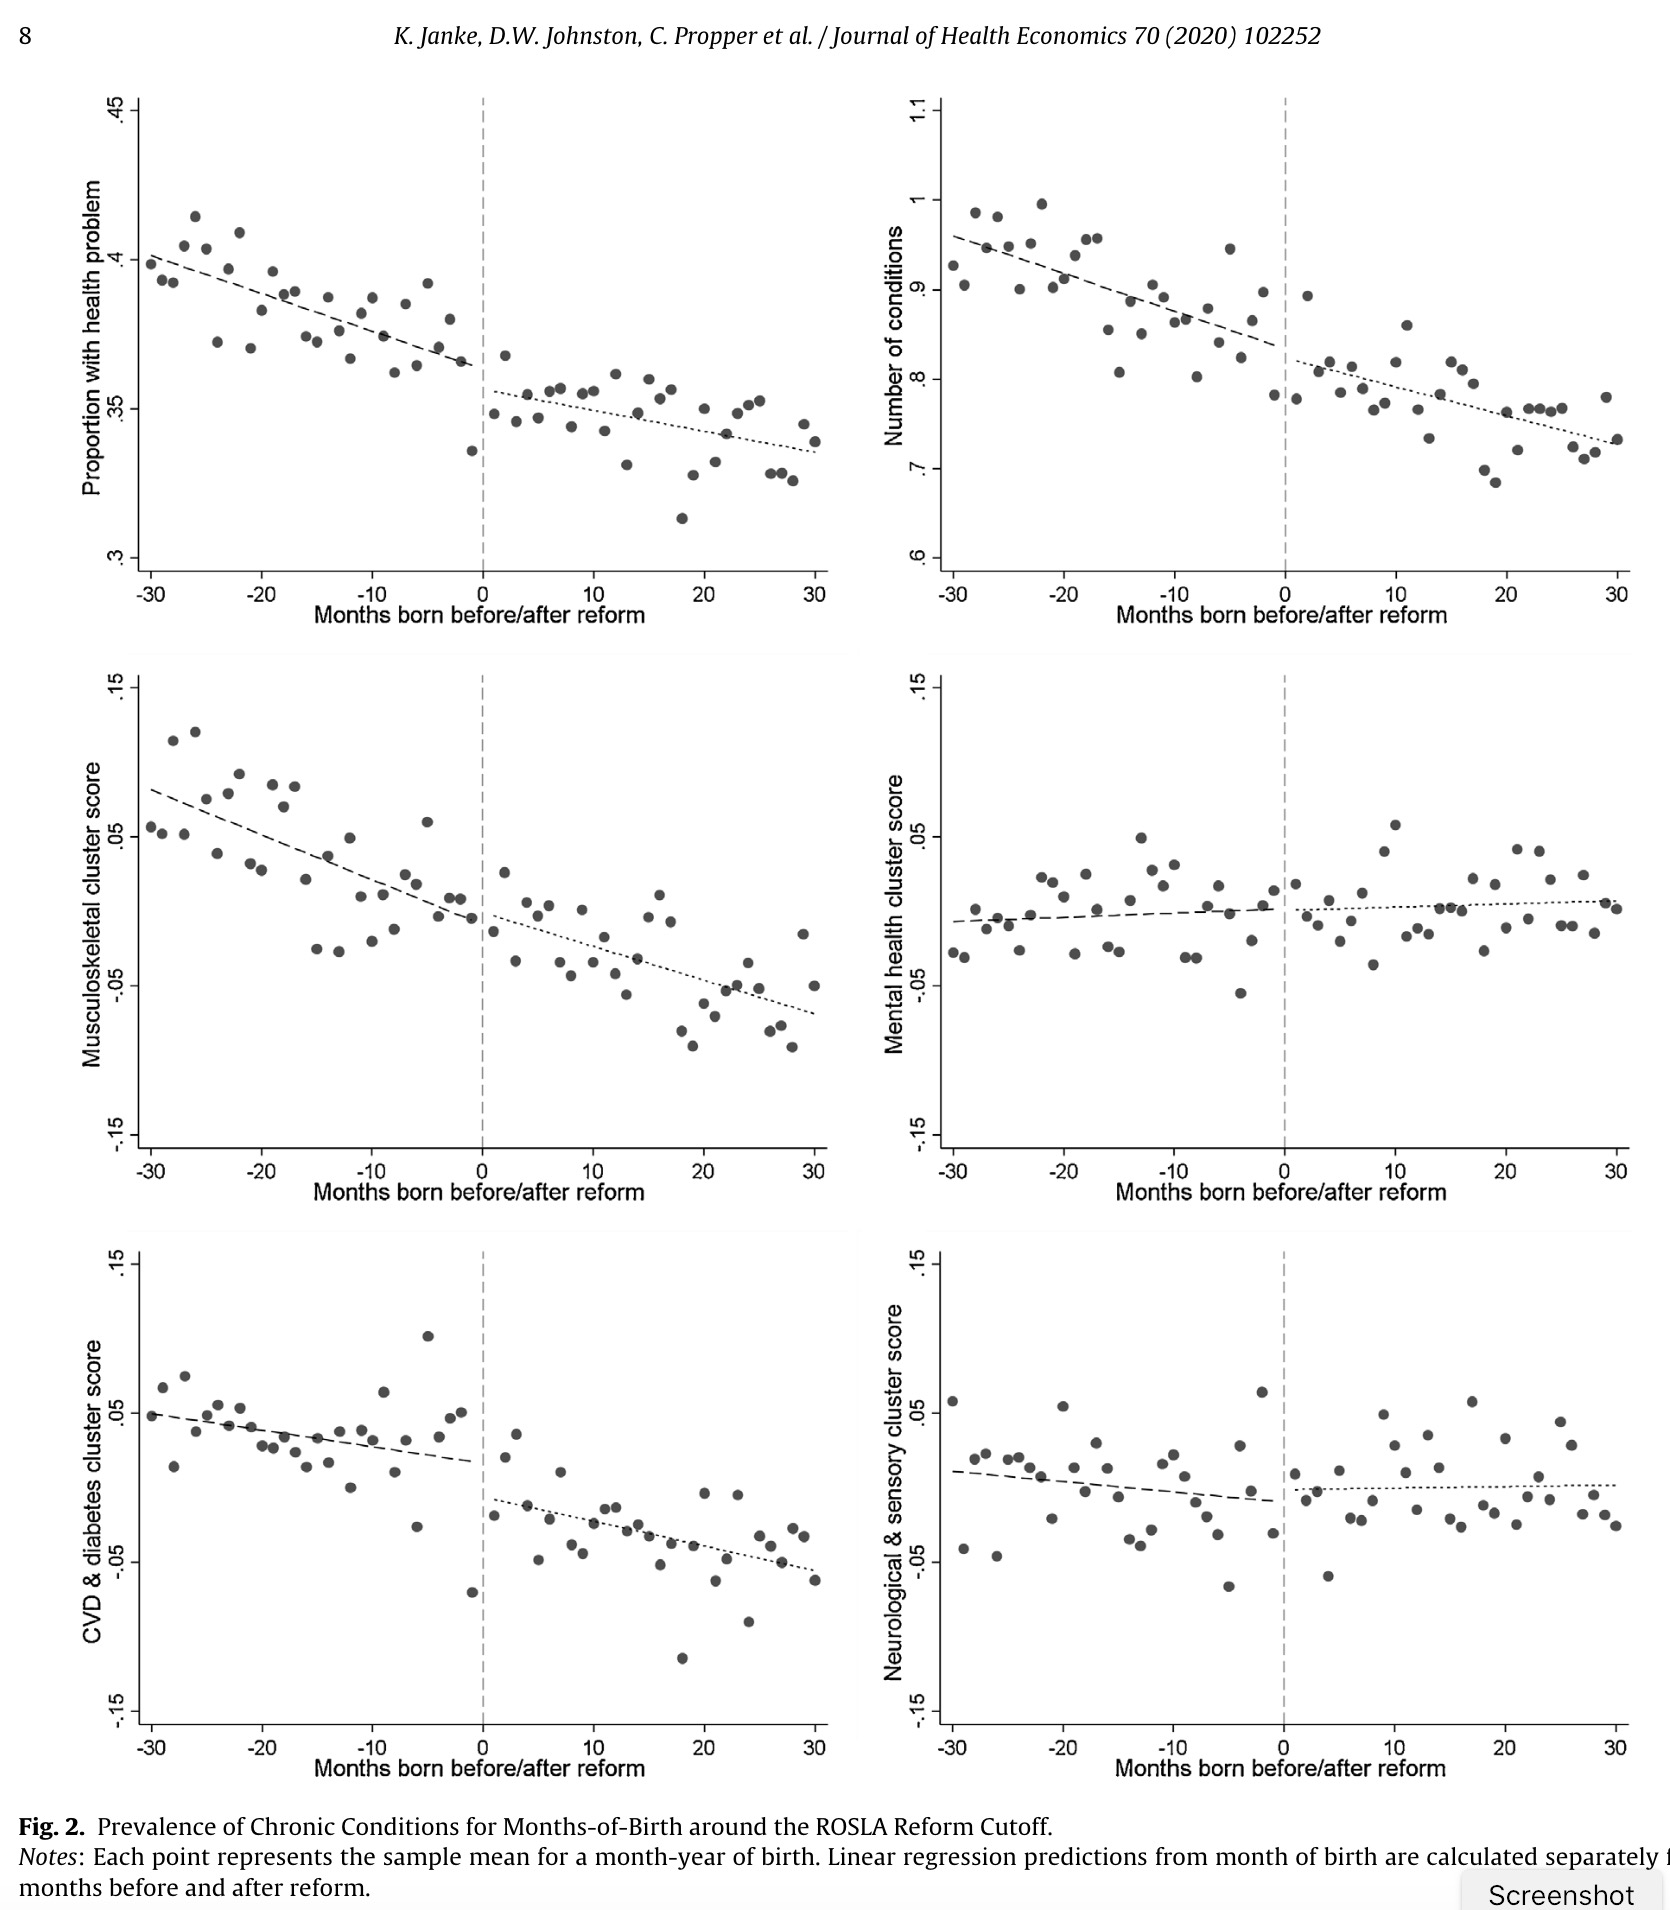
\includegraphics[width=4in]{images/ch3/39.png}
                \caption{Prevalence of Chronic Conditions for Months-of-Birth around the ROSLA Reform Cutoff}
                \label{fig:label}
            \end{figure} 

\begin{itemize}
        \item Another recent paper did the same reform and showed that only the prevalence of cardiovascular diseases was affected by the reform.
\end{itemize}

     \begin{figure}[H]%option [H] means "strictly here"
                \centering
                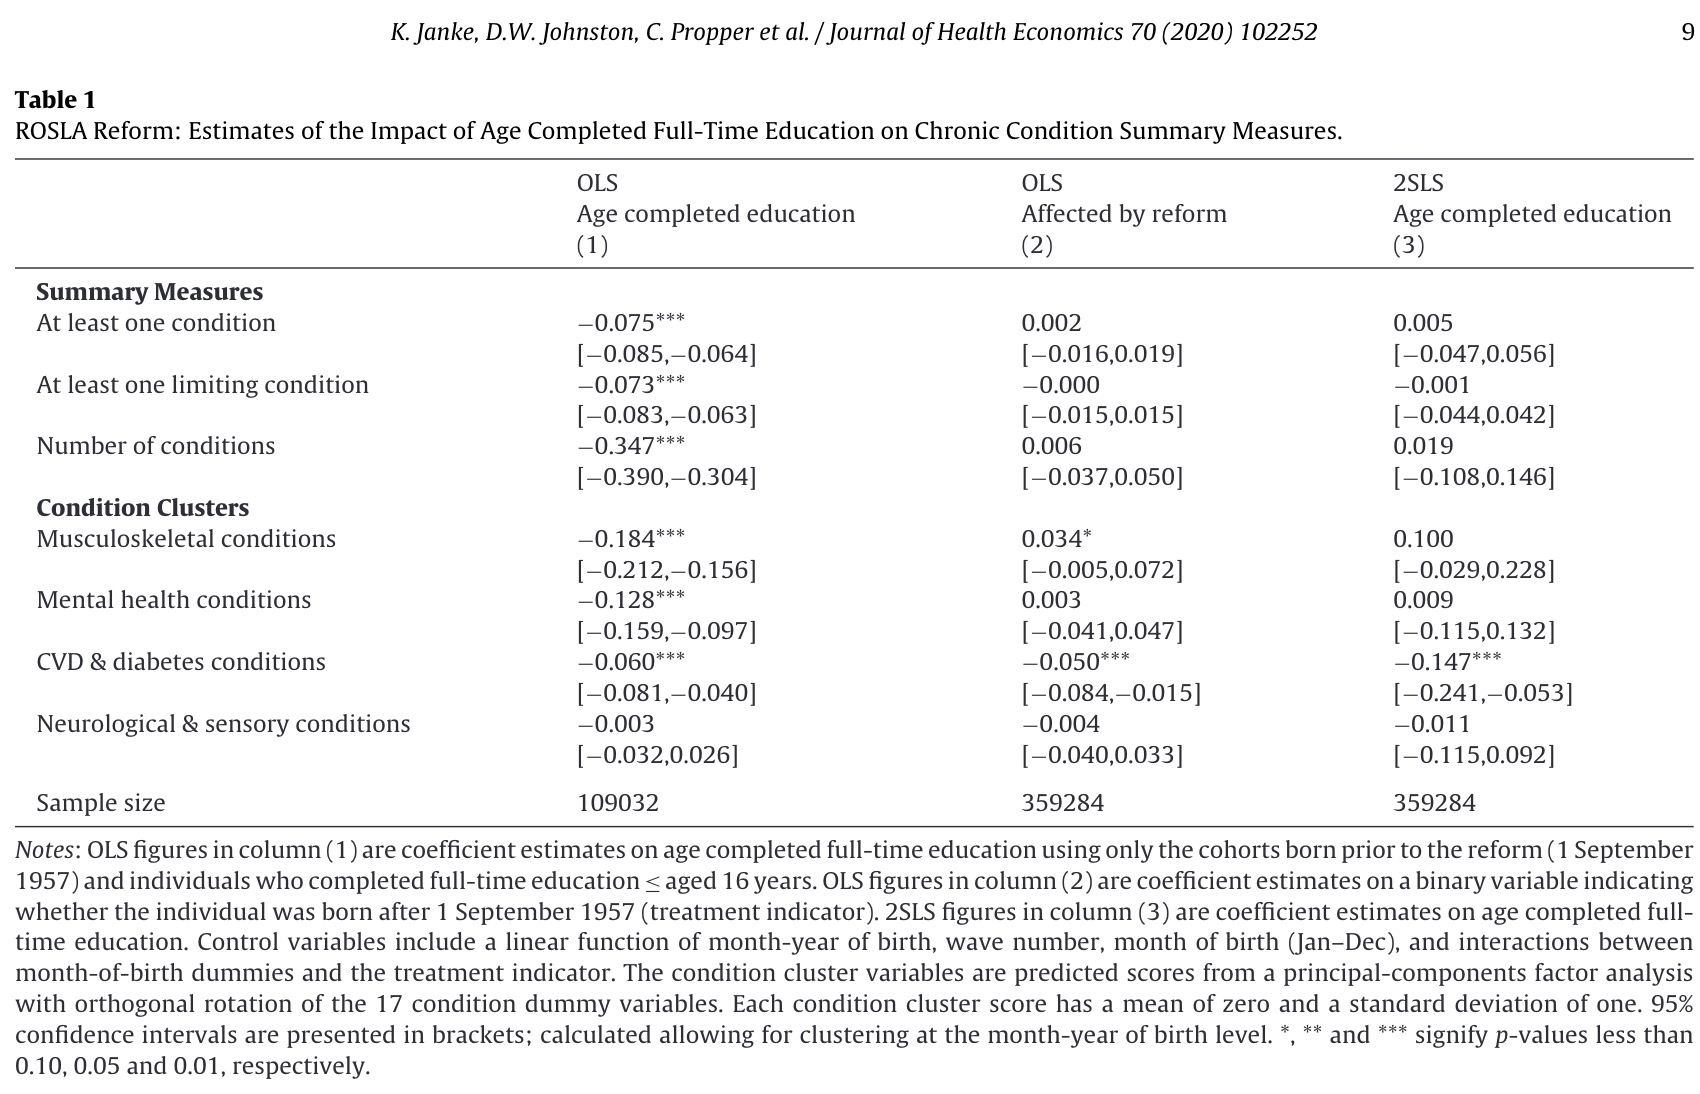
\includegraphics[width=4in]{images/ch3/40.png}
                \caption{ROSLA Reform}
                \label{fig:label}
            \end{figure}        
            
\begin{itemize}
        \item If we directly do OLS regression of education on health, we can see a lot of correlation. However, if we use 2SLS (Regression Discontinuity Design), we see that the coefficients are close to 0 and are statistically insignificant apart from cardiovascular diseases. Therefore, compulsory schooling laws seemed to have little effect on health.
\end{itemize}
        
\subsubsection{Explaining the Gradient}
\begin{enumerate}
    \item Cutler and Lleras-Muney (JHE, 2010)

\begin{itemize}

        \item Cutler and Lleras-Muney (JHE, 2010) examine possible explanations for the relationship between education and health, using several datasets from US and UK. They use OLS regression and see how much the coefficient goes down when adding additional covariates.
        \item They are able to explain two-thirds of the gradient.
        \item "Economic resources" is able to explain 32 percent of the gradient. "Specific knowledge" is able to explain 12 percent of the gradient (US dataset). "Cognitive ability" seems to explain a lot in the UK dataset. "Tastes" and "Personality" explain a little and "social integration" explains somehow.
\end{itemize}
        
\begin{figure}[H]%option [H] means "strictly here"
                \centering
                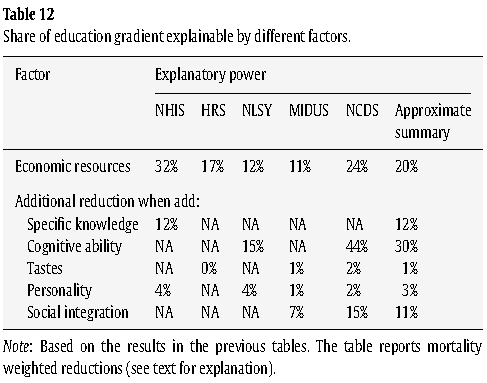
\includegraphics[width=4in]{images/ch3/41.png}
                \caption{Share of education gradient explainable by different factors}
                \label{fig:label}
            \end{figure}
            
\item Conti and Hansman (JHE, 2013)
            
\begin{itemize} 
        \item Conti and Hansman (JHE, 2013) test the robustness of CLM results by using alternative measures of child personality available in the National Child Development Study:
\begin{itemize}
        \item the Rutter Behavior Scale (ages 7, 11 and 16)
        \item the British Social Adjustment Guide (BSAG, ages 7 and 11):
\end{itemize}
        \item CLM results show that adult personality explains very little of the education-health gradient, but Conti and Hansman (JHE, 2013) show that child personality contributes the education-health gradient to an extent nearly as large as cognition. 
        \item Childhood matters.
\end{itemize}
\begin{figure}[H]%option [H] means "strictly here"
                \centering
                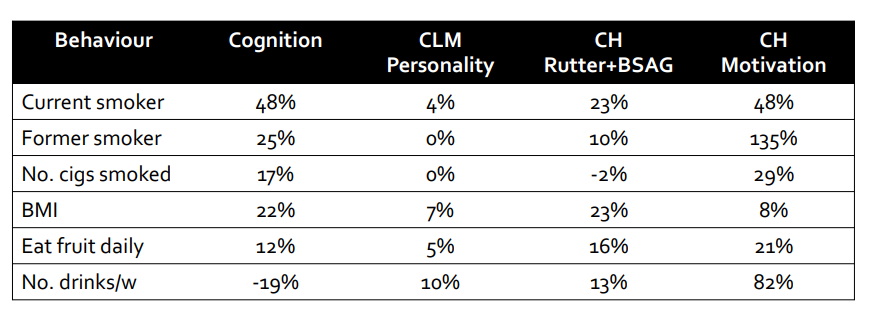
\includegraphics[width=4in]{images/ch3/42.png}
                \caption{How much education-health gradient is explained by cognition, personality and motivation}
                \label{fig:label}
            \end{figure} 
\end{enumerate}


\subsubsection{Child Socioemotional Traits Are Important Determinants of the Gradient}
\begin{figure}[H]%option [H] means "strictly here"
                \centering
                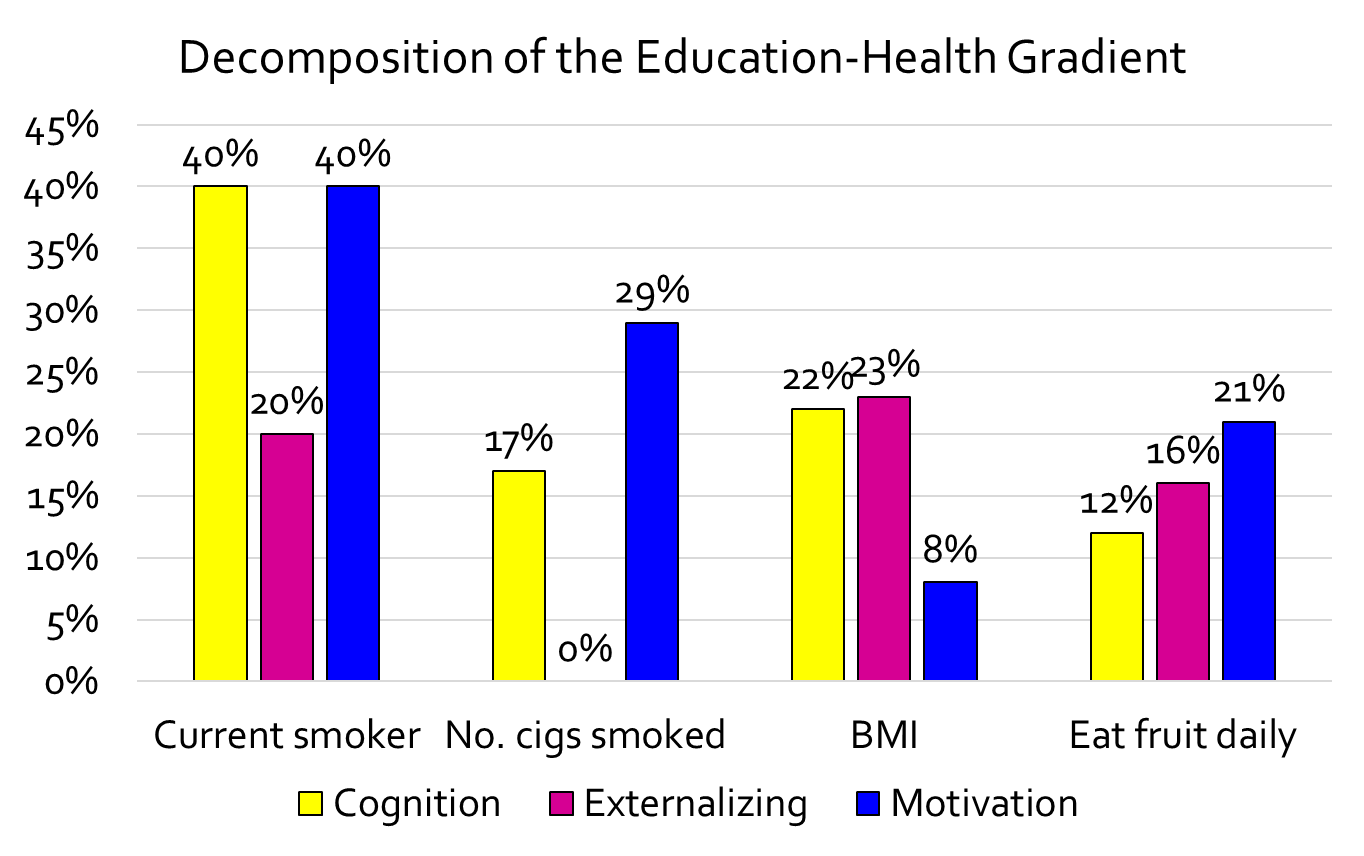
\includegraphics[width=4in]{images/ch3/43.png}
                \caption{Decomposition of the Education-Health Gradient}
                \label{fig:label}
            \end{figure} 

\begin{itemize}
        \item Non-cognitive factors such as externalising and motivation are at least as important as cognition in explaining the gradient.
\end{itemize}

\subsubsection{The Early Origins of the Gradient}

\begin{itemize}
        \item Conti, Heckman et al. (AER, PPS, 2010a,b) decompose observed educational differentials into causal components and components due to selection on early childhood human capital endowments.
        \item They incorporate both the health selection, the social causation and the third factors hypothesis.
        \item They look at the mean effect of education on health (like previous literature) and also at heterogeneity in treatment effects for people with different early childhood endowments.
        \item They quantify the proportion of the educational differential attributed to the causal effect of education vs. early life factors. 
        \item Heckman, Humphries and Veramendi (JPE 2018) extend this framework into a dynamic model of schooling choice and estimate causal effects from multiple levels of schooling. Find substantial continuation value of schooling for high-ability individuals, but not for low ones beyond high school.
        \item Conti et al. use the British Cohort Study (BCS70), a cohort of all individuals born in one week of April 1970 in the United Kingdom.
        \item They estimate a semiparametric structural model of the choice of schooling (decision to stay on at 16) and the causal effect of schooling on a variety of outcomes at age 30: 
        \begin{enumerate}
            \item labour market (wages and employment)
            \item health status (self-reported health, depression and obesity)
            \item health behaviours (smoking, exercise)
        \end{enumerate}
        \item They model three childhood (age 10) endowments as determinants both of education and age 30 outcomes:
        \begin{enumerate}
            \item cognition (e.g. British Ability Scales)
            \item noncognitive traits (e.g. locus of control)
            \item health (height, head circumference)
            \end{enumerate}
          \item We want these three early childhood factors to affect education (if the child is more developed $\Rightarrow$ more able to learn $\Rightarrow$ acquire more education).  Education affects health. Also, these three factors affect health directly. With this structure, health is partly causally affected by education, and partly causally affected by early childhood factors.

          
\begin{figure}[H]%option [H] means "strictly here"
                \centering
                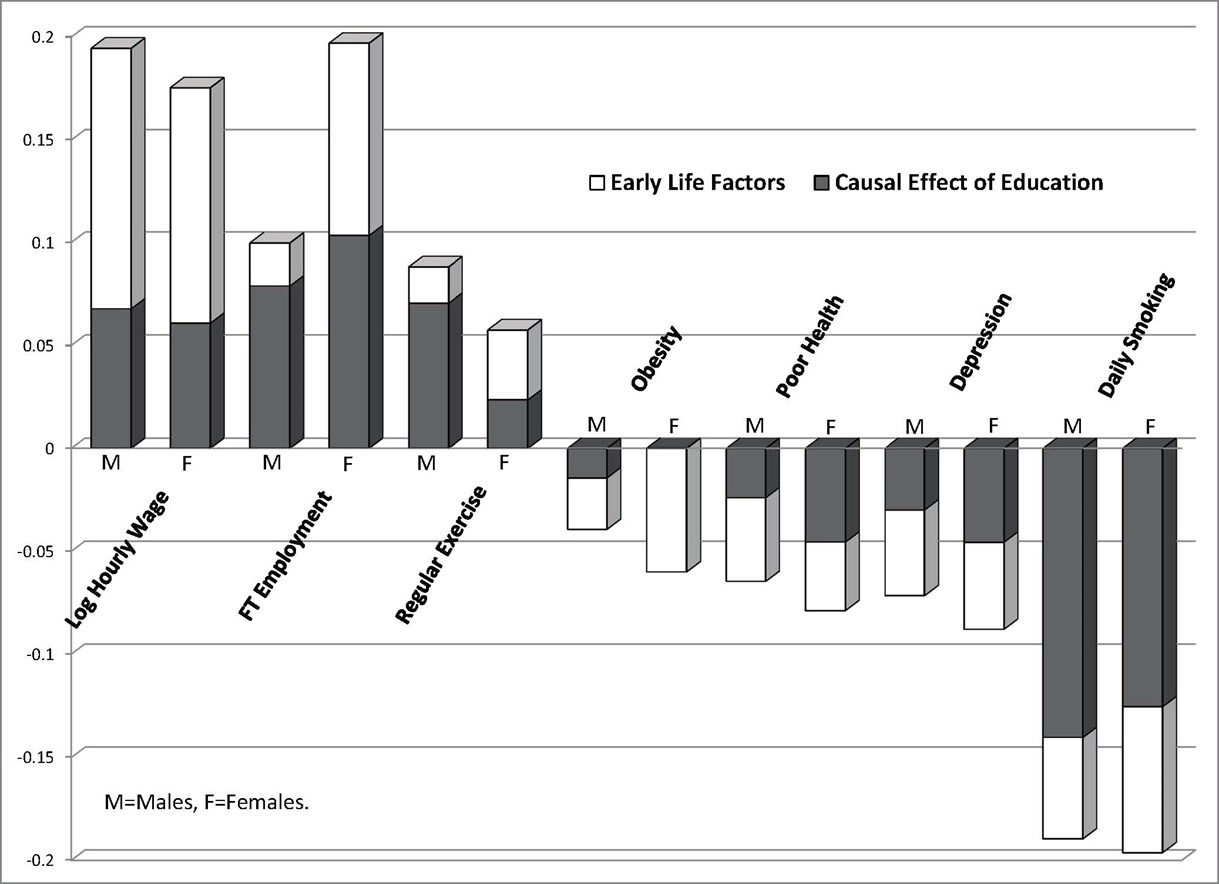
\includegraphics[width=4in]{images/ch3/44.png}
                \caption{How education and early life factors share the causal effects on different health outcomes}
                \label{fig:label}
            \end{figure}        
\end{itemize}

\begin{itemize}
\item Education explains nearly nothing about the obesity of females. For daily smoking, education matters more than early life factors.
\end{itemize}

\subsubsection{The Effects of Childhood Endowments on the Probability of being a Daily Smoker at Age 30}    
\begin{figure}[H]%option [H] means "strictly here"
                \centering
                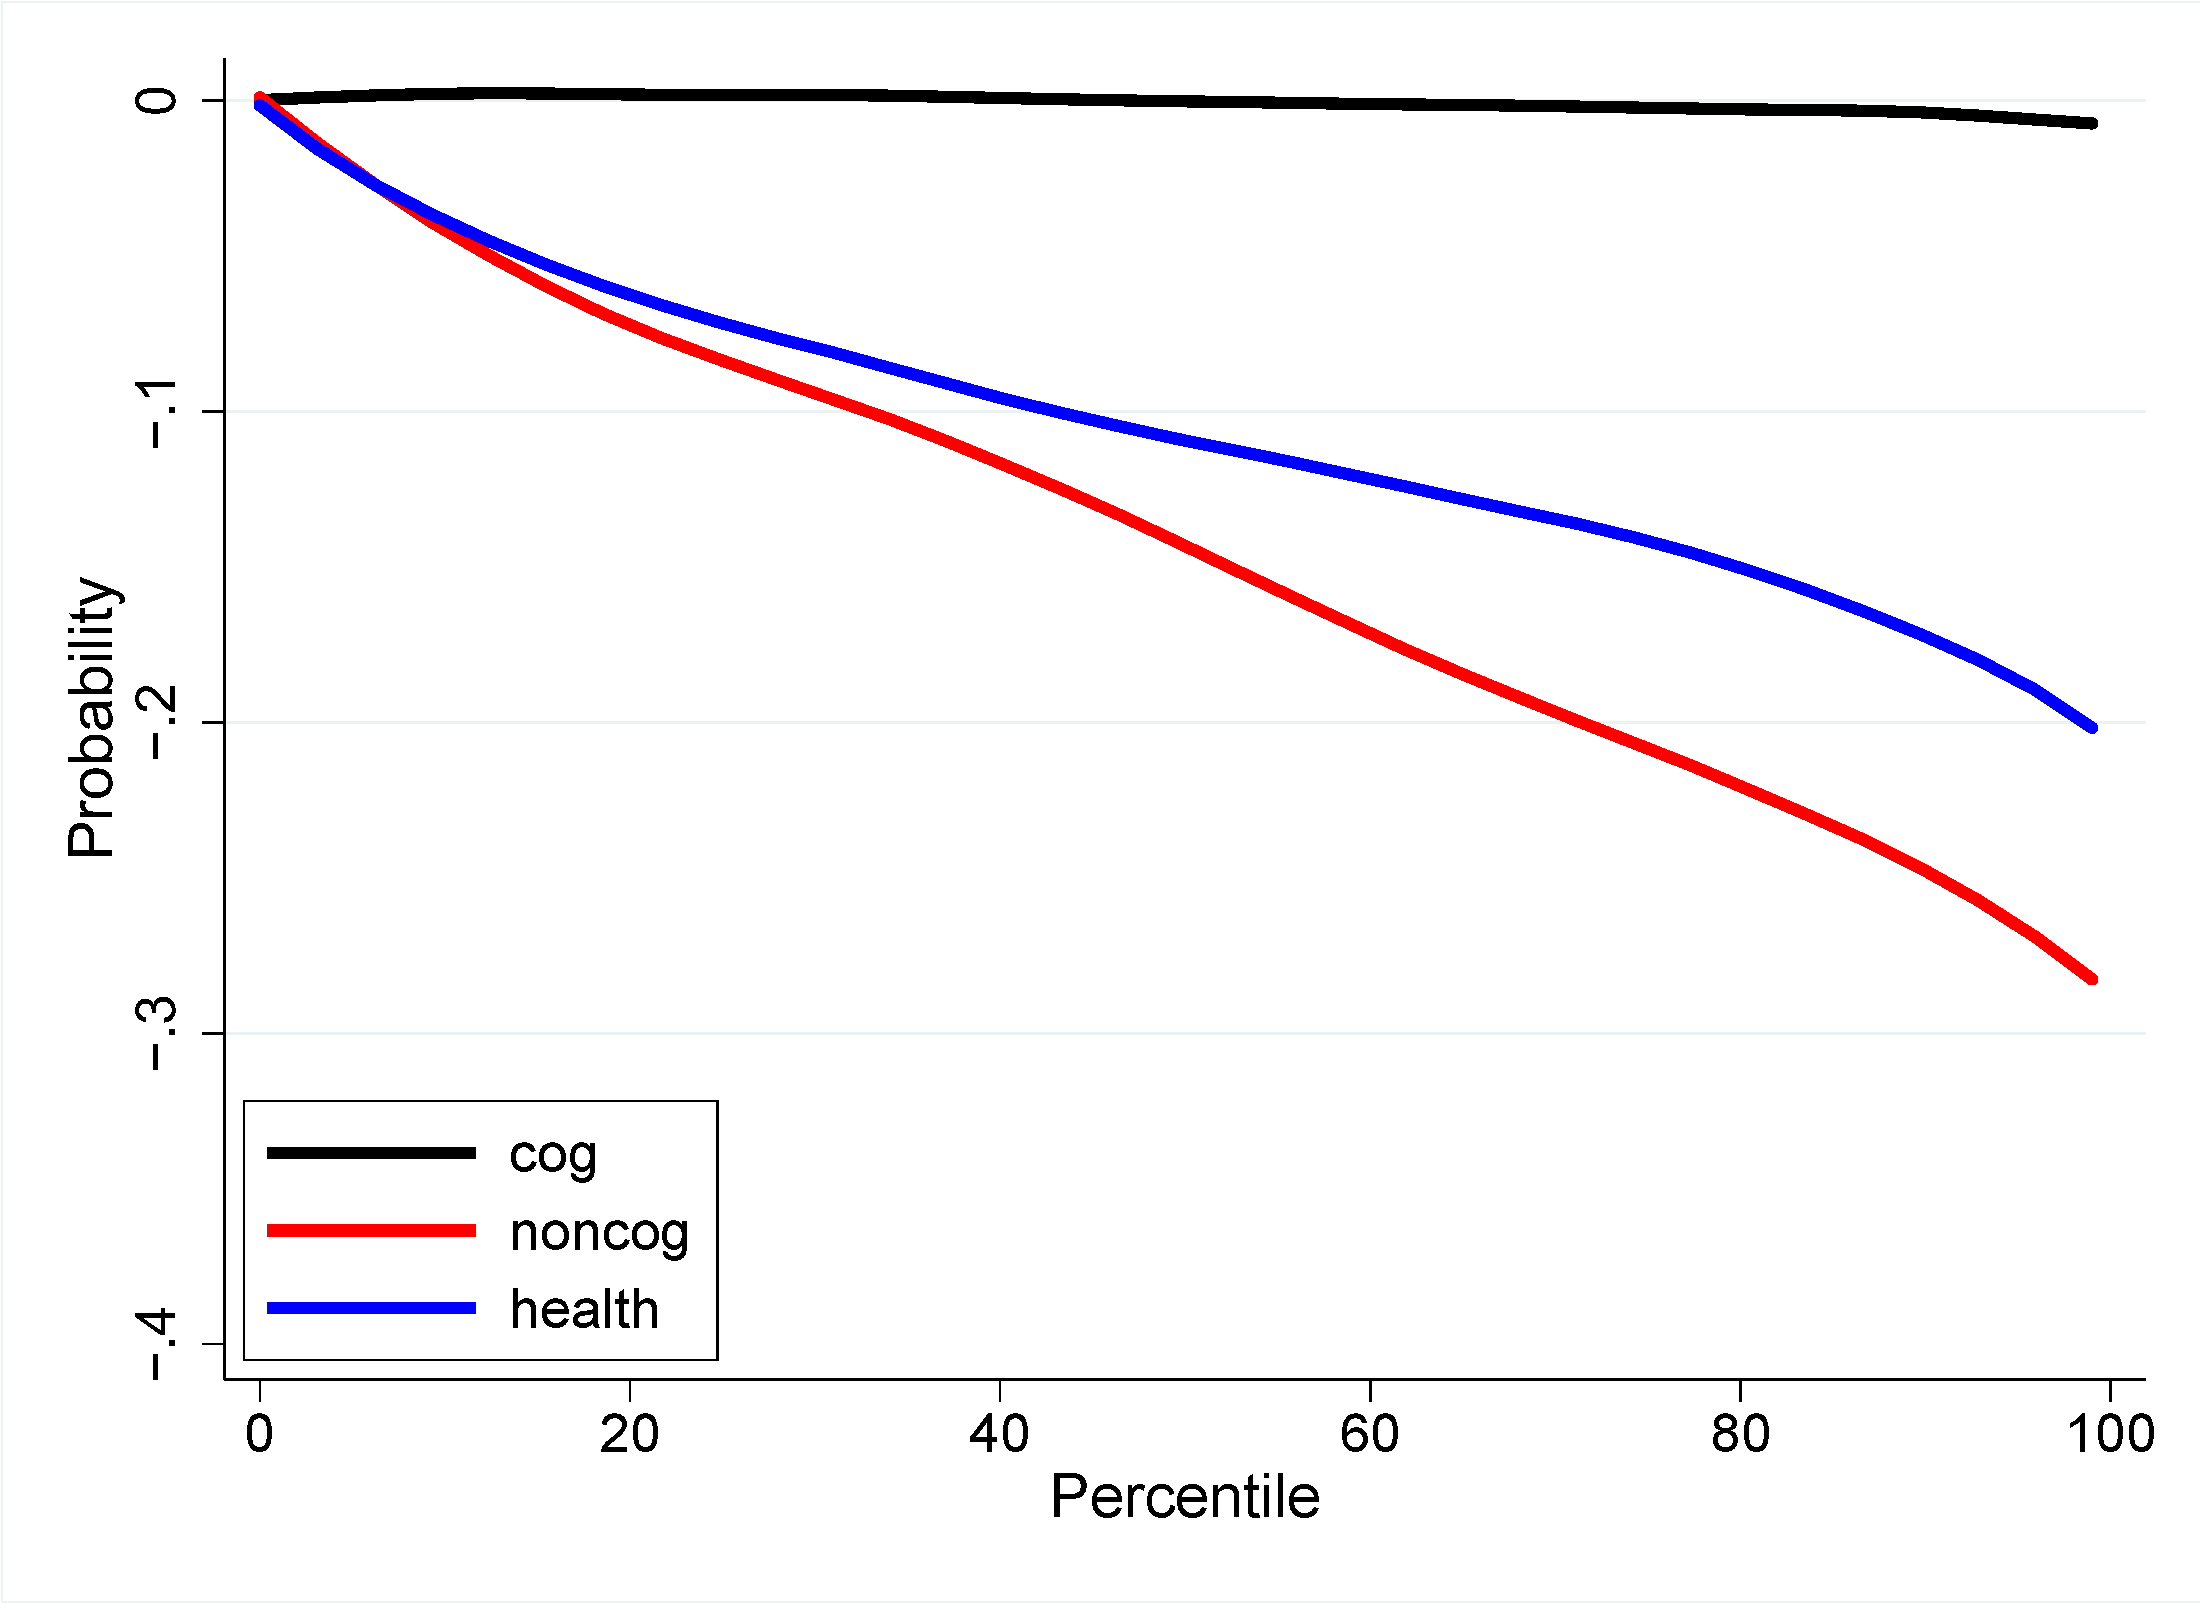
\includegraphics[width=4in]{images/ch3/45.png}
                \caption {The Effects of Childhood Endowments on the Probability of
being a Daily Smoker at Age 30}
                \label{fig:label}
            \end{figure} 

\begin{itemize}
    \item Cognition doesn't affect smoking. Non-cognitive factors (e.g. self-regulation and motivation) and physical health are equally important determinants of smoking.
\end{itemize}

\subsubsection{The Effects of Childhood Endowments on the Probability of being Obese at Age 30}    
\begin{figure}[H]%option [H] means "strictly here"
                \centering
                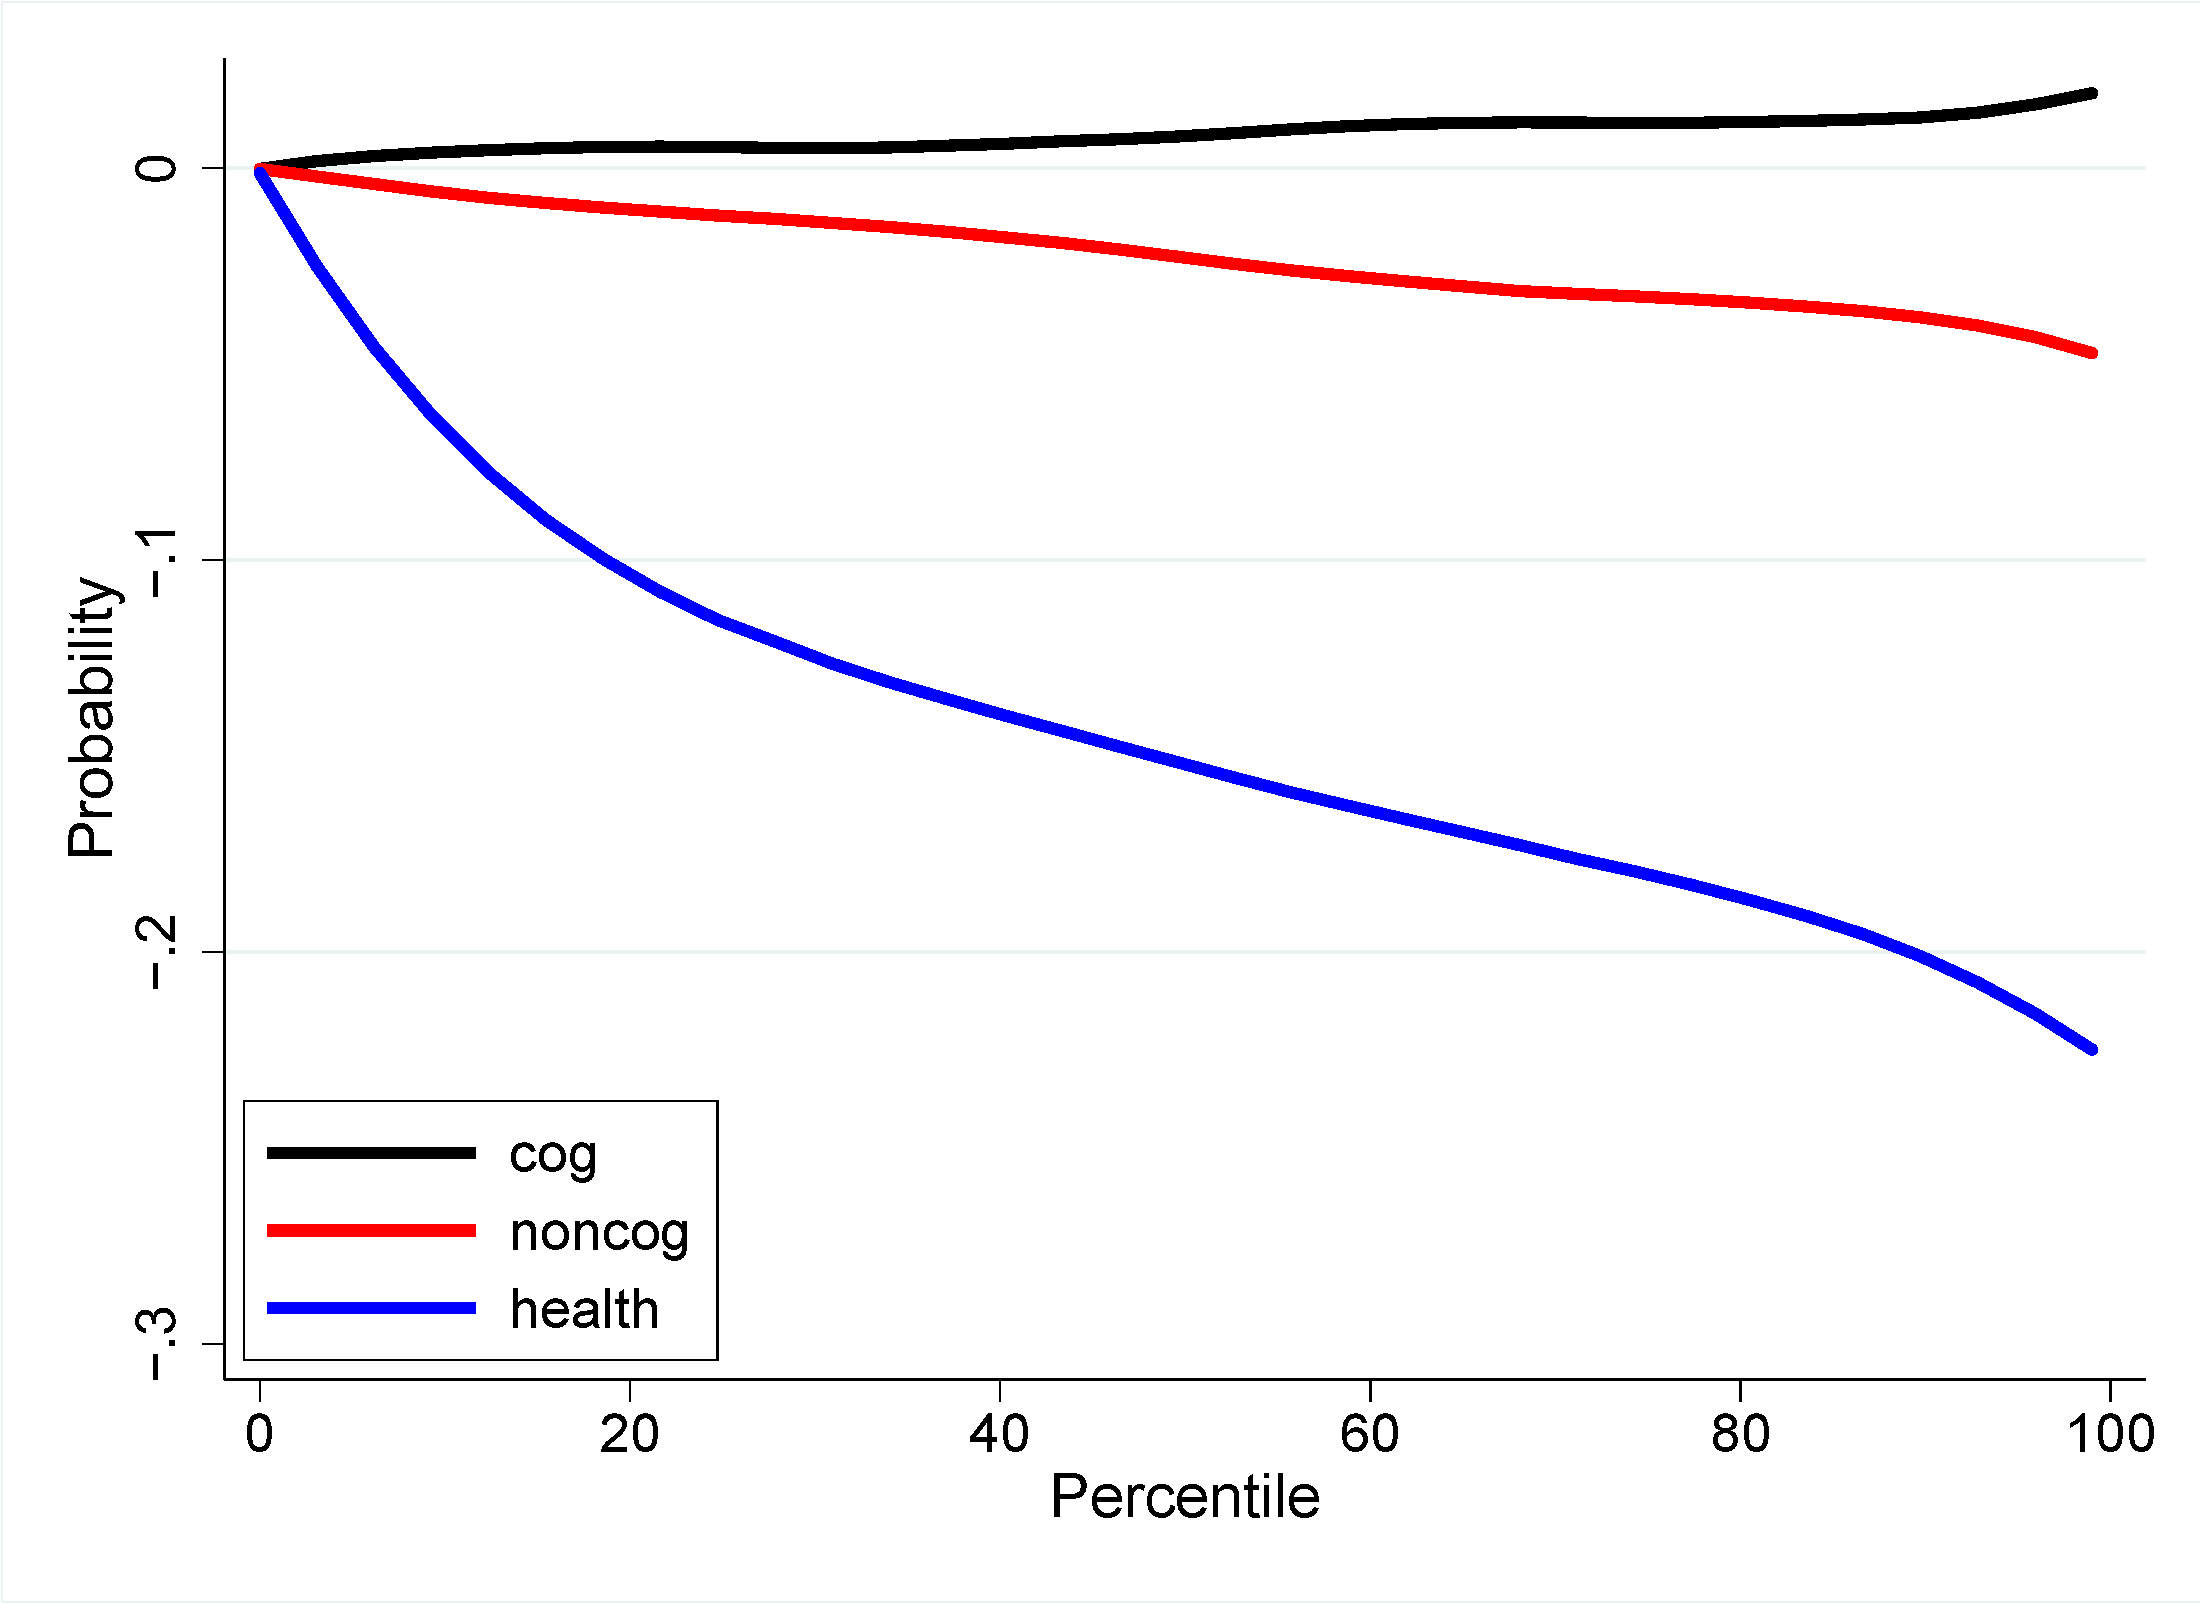
\includegraphics[width=4in]{images/ch3/46.png}
                \caption {The Effects of Childhood Endowments on the Probability of
being Obese at Age 30}
                \label{fig:label}
            \end{figure} 
            
\begin{itemize}
    \item Cognition matters little. Non-cognitive explains a little bit. Early physical health is the most important determinant of obesity.
\end{itemize}

\subsubsection{Heterogeneity in the Effects of Education on Smoking}    
\begin{figure}[H]%option [H] means "strictly here"
                \centering
                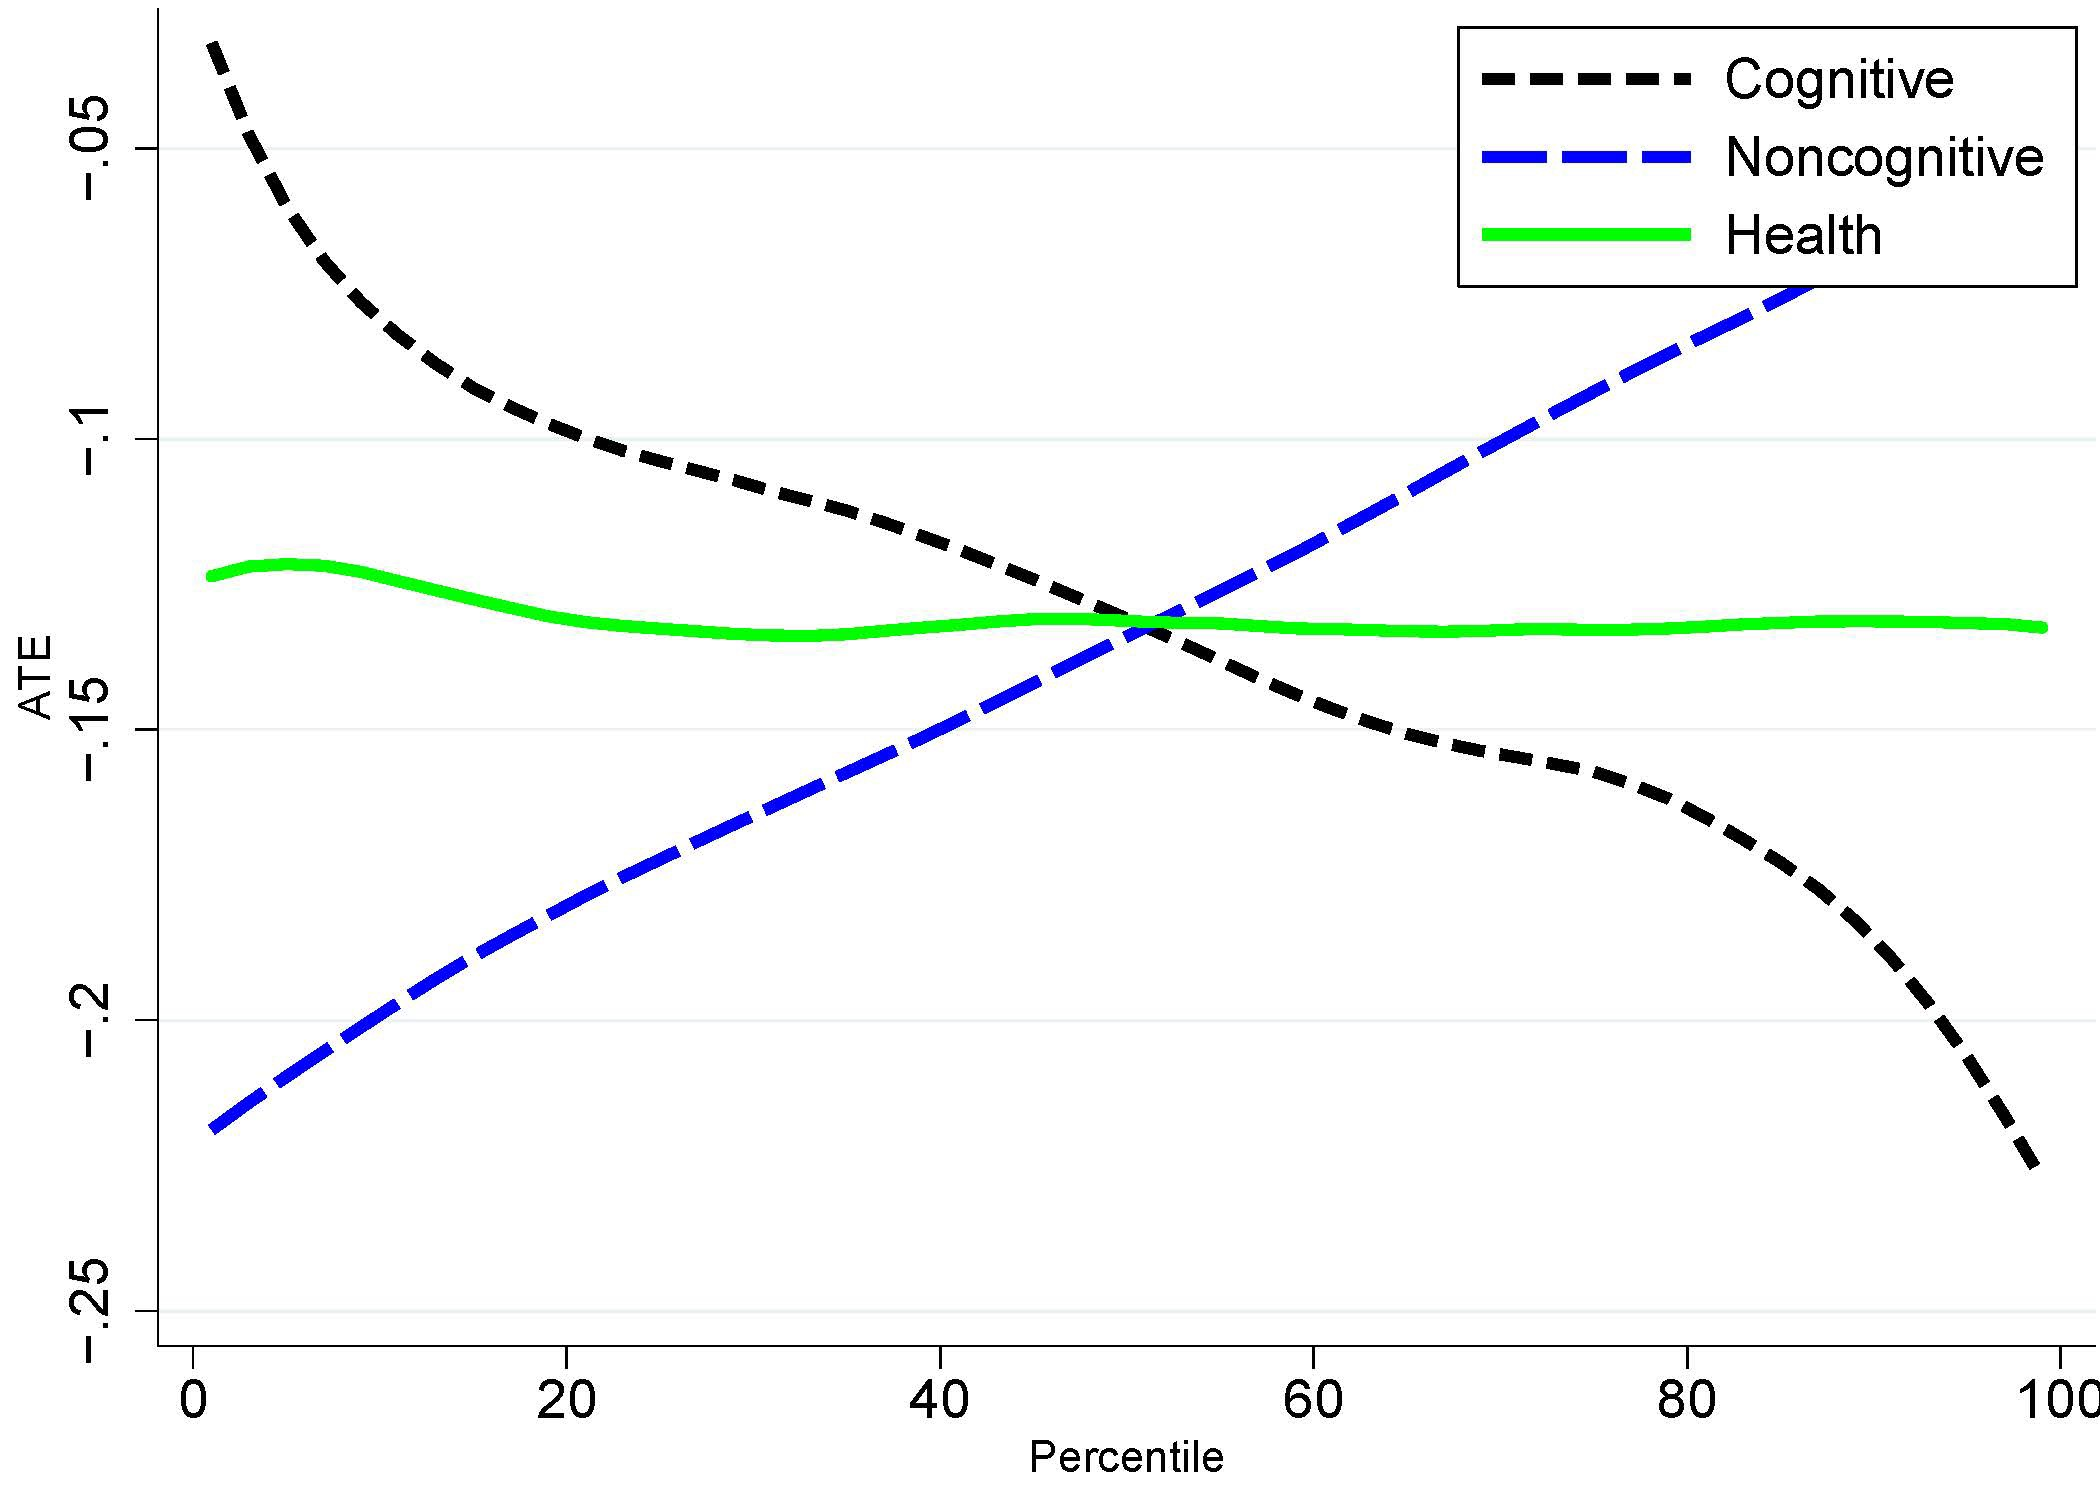
\includegraphics[width=4in]{images/ch3/47.png}
                \caption {Heterogeneity in the Effects of Education on Smoking}
                \label{fig:label}
            \end{figure} 
            
\begin{itemize}
    \item The effects of later intervention (education) on smoking depend on the effects of early child interventions.
    \item Heterogeneity in the effects (ATE=Average Treatment Effect) of post-compulsory education on smoking at age 30 as function of early endowments: education compensates for low early non-cognitive endowments and reinforces high early cognitive endowments.
    \item First, the beneficial effect of education (ATE) is much bigger at the top of the cognitive ability distribution. This is particularly interesting in the case of smoking, as it is consistent with the interpretation that the information content on the dangers of smoking provided by post-compulsory education needs to be combined with the capacity to process that information in order to be effective. Second,  education compensates for poor noncognitive ability (increase motivation). Third, there is no heterogeneity in the effect of education along the distribution of the health endowment. 
 
\end{itemize}

\subsubsection{Evidence from a Dynamic Model}  
\begin{figure}[H]%option [H] means "strictly here"
                \centering
                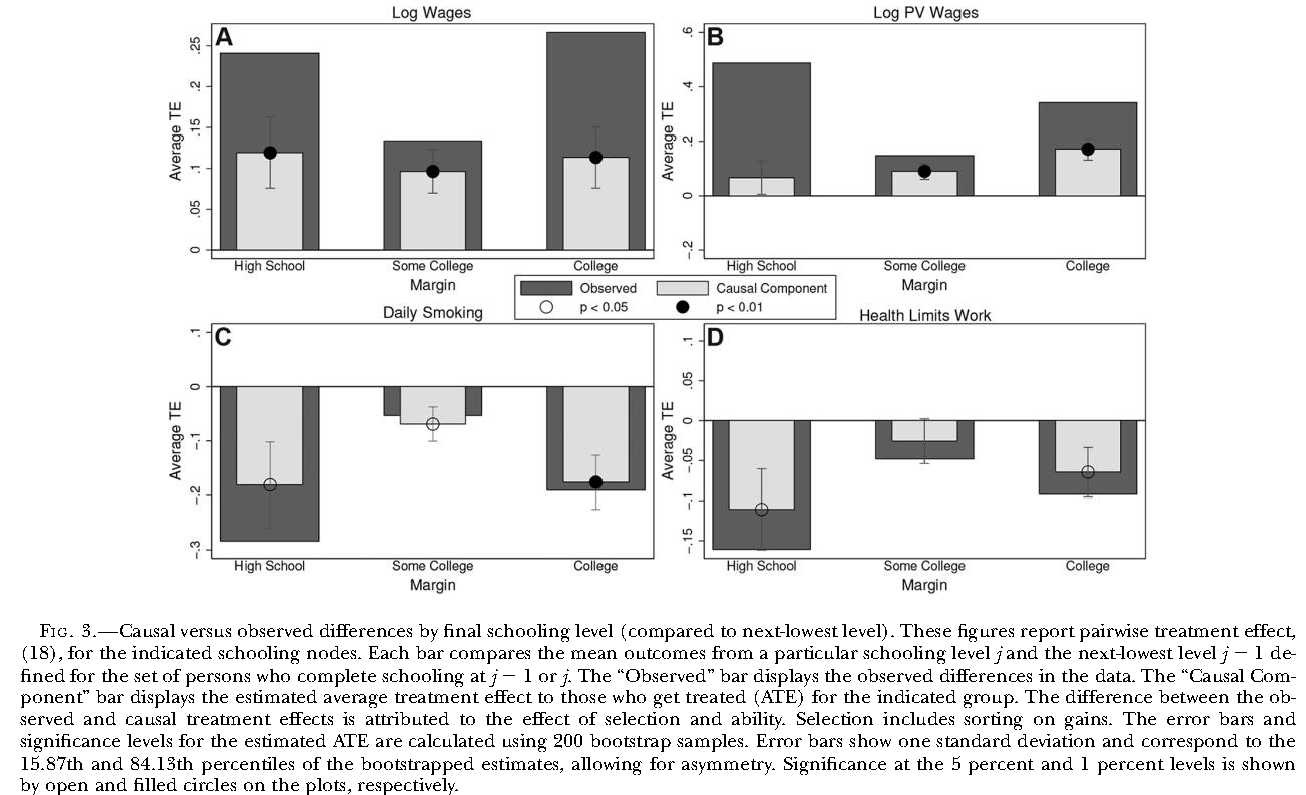
\includegraphics[width=5in]{images/ch3/48.png}
                \caption {Evidence from a Dynamic Model}
                \label{fig:label}
            \end{figure}
\begin{itemize}
    \item How additional level of education affects wages and health compared to previous education level
    \item The shaded regions labelled “Observed” are the raw differences found in the data. The estimated average causal effects (displayed in the light blocks) are large and statistically significant for all outcomes except for the log PV wages for graduating from high school (compared to dropping out). For example, the left-most bar in panel A can be interpreted as follows: while high school graduates make, on average, 24 log points higher wages than high school dropouts, we find that the average causal effect of graduating from high school is, on average, 12 log points for the same population.
    \item Panel C: The biggest reduction in smoking was seen in people with high school degrees compared to those without, and more than half of the effect can be explained by the causal effect of education. However, most of the reduction in smoking can be explained by the causal effect of education for people with college degrees compared to those without. The causal component depends on each level of education (as well as the quality of education).
\end{itemize}

            

\subsubsection{The State of the Literature}  
\begin{itemize}
    \item Recent review “The Effect of Education on Health and Mortality: A Review of Experimental and Quasi-Experimental Evidence” by T. Galama, A. LlerasMuney, H. van Kippersluis, Oxford Research Encyclopedia of Economics and Finance (2018).
    \item Review evidence on the two most common preventable causes of mortality: smoking and obesity.
    \item \textcolor{red}{“There is no convincing evidence of an effect of education on obesity, and the effects on smoking are only apparent when schooling reforms affect individuals’ track or their peer group, but not when they simply increase the duration of schooling.”}
    \item “An effect of education on mortality exists in some contexts but not in others, and seem to depend on: (a) gender; (b) the labour market returns to education; (c) the quality of education; (d) whether education affects peers’ quality.”
    \item Important step forward would be to understand the quality and content of further education, years beyond the minimum school leaving age, and both short-, medium-, and long-term outcomes.
\end{itemize}

\begin{figure}[H]%option [H] means "strictly here"
                \centering
                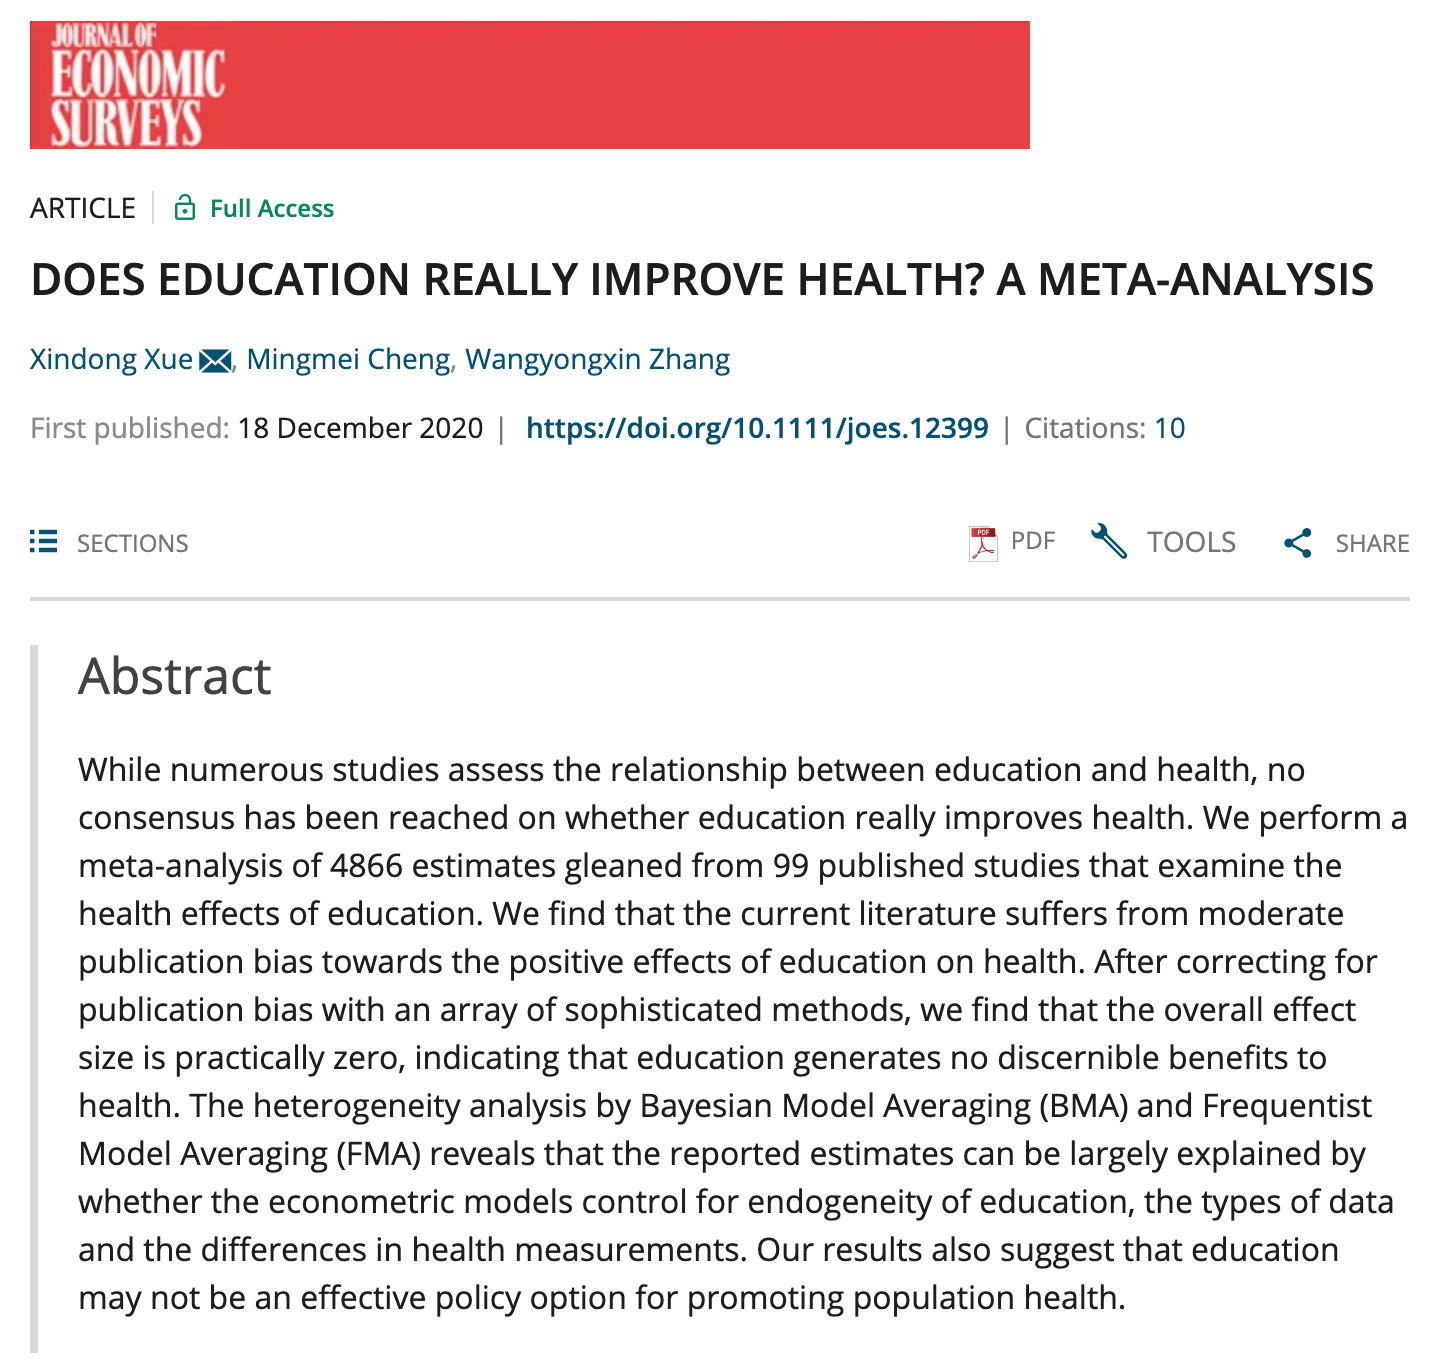
\includegraphics[width=3in]{images/ch3/49.png}
                \caption {Does education really improve health? A Meta-Analysis}
                \label{fig:label}
            \end{figure}

\begin{itemize}
    \item Publication bias towards the positive effects of education on health.
\end{itemize}

\subsubsection{Where Next?}
\begin{itemize}
    \item Grossman (NBER wp 21609, 2015) “The Relationship between Health and Schooling: What’s New?” concludes “There is enough conflicting evidence in the studies that I have reviewed to warrant more research on the question of whether more schooling does in fact cause better health outcomes.”
    \item Among promising areas of current and future research:
    \begin{itemize}
    \item Does schooling quality matter?
    \item What are the mechanisms via which schooling influences health and health behaviours?
    \item What is the role of genes?
    \item What is the role of subjective expectations of returns?
    \end{itemize}
\end{itemize}

\section{Full Bibliography}
\begin{itemize}
\item Barcellos et al. (2018). PNAS. Education can reduce health differences related to genetic risk of obesity.
\item Clark, D. and Royer, H. (2013). The Effect of Education on Adult Mortality: Evidence from Britain. American Economic Review, 106(6),
2087-2120.
\item Conti, G., and Hansman, C. (2013). Personality and the education–health gradient: A note on “Understanding differences in health
behaviours by education”. Journal of health economics, 32(2), 480-485.
\item Conti, G. and Heckman, J.J. (2010). Understanding the Early Origins of the Education-Health Gradient: A Framework That Can Also Be Applied to Analyze Gene-Environment Interactions. Perspectives on Psychological Science, 5(5), 585-605.
\item Conti,G., Heckman,J.J. and Urzua, S. (2010).The Education-Health Gradient. American Economic Review P P, 100(2), 234-238.
\item Cutler, D. M., and Lleras-Muney, A. (2010). Understanding differences in health behaviours by education. Journal of health economics,
29(1), 1-28.
• [Erlich, I., and H. Chuma (1990) “A model of the demand for longevity and the value of life extensions”, Journal of Political Economy
98:761-782.]
\item Galama,T. and H. van Kippersluis (2018).A Theory of Socioeconomic Disparities in Health Over the Life Cycle, Economic Journal.
\item Galama, Titus J. and Lleras-Muney, Adriana and van Kippersluis, Hans, The Effect of Education on Health and Mortality: A Review of
Experimental and Quasi-Experimental Evidence, Oxford Encyclopedia of Economics and Finance.
\item Gilleskie, D. (2008). Health Capital: Theory and Empirical Evidence. Incentives and Choice in Health Care MIT Press: Cambridge, MA.
\item Grossman, M. (1972). On the concept of health capital and the demand for health. Journal of Political economy, 80(2), 223-255.
\item Grossman, M. (2000). The human capital model. Handbook of health economics, 1, 347-408.
\item Grossman, M. (2015).The Relationship between Health and Schooling: What’s New? NBER wp 21609.
\item Heckman, J. J. (2007). The economics, technology, and neuroscience of human capability formation. Proceedings of the national
Academy of Sciences, 104(33), 13250-13255.
\item Heckman, J.J., J.E. Humphries and G. Veramendi (2018). Returns to Education: The Causal Effects of Education on Earnings, Health
and Smoking. Journal of Political Economy, October S1.
\item Janke, K., D.Johnston, C. Propper and M. Shields (2018).The Causal Effect of Education on Chronic Health Conditions. IZA DP 11353.
\item Lleras-Muney, A. (2005). The relationship between education and adult mortality in the United States. The Review of Economic
Studies, 72(1), 189-221.
\item Lundborg, P. (2013).The health returns to schooling—what can we learn from twins? Journal of population economics, 26(2), 673-701 
\end{itemize}